\documentclass[twoside]{book}

% Packages required by doxygen
\usepackage{calc}
\usepackage{doxygen}
\usepackage{graphicx}
\usepackage[utf8]{inputenc}
\usepackage{makeidx}
\usepackage{multicol}
\usepackage{multirow}
\usepackage{textcomp}
\usepackage[table]{xcolor}

% Font selection
\usepackage[T1]{fontenc}
\usepackage{mathptmx}
\usepackage[scaled=.90]{helvet}
\usepackage{courier}
\usepackage{amssymb}
\usepackage{sectsty}
\renewcommand{\familydefault}{\sfdefault}
\allsectionsfont{%
  \fontseries{bc}\selectfont%
  \color{darkgray}%
}
\renewcommand{\DoxyLabelFont}{%
  \fontseries{bc}\selectfont%
  \color{darkgray}%
}

% Page & text layout
\usepackage{geometry}
\geometry{%
  a4paper,%
  top=2.5cm,%
  bottom=2.5cm,%
  left=2.5cm,%
  right=2.5cm%
}
\tolerance=750
\hfuzz=15pt
\hbadness=750
\setlength{\emergencystretch}{15pt}
\setlength{\parindent}{0cm}
\setlength{\parskip}{0.2cm}
\makeatletter
\renewcommand{\paragraph}{%
  \@startsection{paragraph}{4}{0ex}{-1.0ex}{1.0ex}{%
    \normalfont\normalsize\bfseries\SS@parafont%
  }%
}
\renewcommand{\subparagraph}{%
  \@startsection{subparagraph}{5}{0ex}{-1.0ex}{1.0ex}{%
    \normalfont\normalsize\bfseries\SS@subparafont%
  }%
}
\makeatother

% Headers & footers
\usepackage{fancyhdr}
\pagestyle{fancyplain}
\fancyhead[LE]{\fancyplain{}{\bfseries\thepage}}
\fancyhead[CE]{\fancyplain{}{}}
\fancyhead[RE]{\fancyplain{}{\bfseries\leftmark}}
\fancyhead[LO]{\fancyplain{}{\bfseries\rightmark}}
\fancyhead[CO]{\fancyplain{}{}}
\fancyhead[RO]{\fancyplain{}{\bfseries\thepage}}
\fancyfoot[LE]{\fancyplain{}{}}
\fancyfoot[CE]{\fancyplain{}{}}
\fancyfoot[RE]{\fancyplain{}{\bfseries\scriptsize Generated on Fri Feb 14 2014 18\-:31\-:04 for Tetris by Doxygen }}
\fancyfoot[LO]{\fancyplain{}{\bfseries\scriptsize Generated on Fri Feb 14 2014 18\-:31\-:04 for Tetris by Doxygen }}
\fancyfoot[CO]{\fancyplain{}{}}
\fancyfoot[RO]{\fancyplain{}{}}
\renewcommand{\footrulewidth}{0.4pt}
\renewcommand{\chaptermark}[1]{%
  \markboth{#1}{}%
}
\renewcommand{\sectionmark}[1]{%
  \markright{\thesection\ #1}%
}

% Indices & bibliography
\usepackage{natbib}
\usepackage[titles]{tocloft}
\setcounter{tocdepth}{3}
\setcounter{secnumdepth}{5}
\makeindex

% Hyperlinks (required, but should be loaded last)
\usepackage{ifpdf}
\ifpdf
  \usepackage[pdftex,pagebackref=true]{hyperref}
\else
  \usepackage[ps2pdf,pagebackref=true]{hyperref}
\fi
\hypersetup{%
  colorlinks=true,%
  linkcolor=blue,%
  citecolor=blue,%
  unicode%
}

% Custom commands
\newcommand{\clearemptydoublepage}{%
  \newpage{\pagestyle{empty}\cleardoublepage}%
}


%===== C O N T E N T S =====

\begin{document}

% Titlepage & ToC
\hypersetup{pageanchor=false}
\pagenumbering{roman}
\begin{titlepage}
\vspace*{7cm}
\begin{center}%
{\Large Tetris }\\
\vspace*{1cm}
{\large Generated by Doxygen 1.8.6}\\
\vspace*{0.5cm}
{\small Fri Feb 14 2014 18:31:04}\\
\end{center}
\end{titlepage}
\clearemptydoublepage
\tableofcontents
\clearemptydoublepage
\pagenumbering{arabic}
\hypersetup{pageanchor=true}

%--- Begin generated contents ---
\chapter{Hierarchical Index}
\section{Class Hierarchy}
This inheritance list is sorted roughly, but not completely, alphabetically\-:\begin{DoxyCompactList}
\item \contentsline{section}{box}{\pageref{classbox}}{}
\item \contentsline{section}{Cube}{\pageref{class_cube}}{}
\item Frame\-Listener\begin{DoxyCompactList}
\item \contentsline{section}{Base\-Application}{\pageref{class_base_application}}{}
\begin{DoxyCompactList}
\item \contentsline{section}{Project\-One}{\pageref{class_project_one}}{}
\end{DoxyCompactList}
\end{DoxyCompactList}
\item Key\-Listener\begin{DoxyCompactList}
\item \contentsline{section}{Base\-Application}{\pageref{class_base_application}}{}
\end{DoxyCompactList}
\item \contentsline{section}{l\-Shape}{\pageref{classl_shape}}{}
\item \contentsline{section}{l\-Shape\-Opp}{\pageref{classl_shape_opp}}{}
\item Mouse\-Listener\begin{DoxyCompactList}
\item \contentsline{section}{Base\-Application}{\pageref{class_base_application}}{}
\end{DoxyCompactList}
\item Panel\-Colors\begin{DoxyCompactList}
\item \contentsline{section}{My\-Simple\-Demo\-Panel\-Colors}{\pageref{struct_my_simple_demo_panel_colors}}{}
\end{DoxyCompactList}
\item Sdk\-Tray\-Listener\begin{DoxyCompactList}
\item \contentsline{section}{Base\-Application}{\pageref{class_base_application}}{}
\end{DoxyCompactList}
\item \contentsline{section}{t\-Shape}{\pageref{classt_shape}}{}
\item \contentsline{section}{t\-Shape\-Opp}{\pageref{classt_shape_opp}}{}
\item Window\-Event\-Listener\begin{DoxyCompactList}
\item \contentsline{section}{Base\-Application}{\pageref{class_base_application}}{}
\end{DoxyCompactList}
\item \contentsline{section}{z\-Shape}{\pageref{classz_shape}}{}
\end{DoxyCompactList}

\chapter{Class Index}
\section{Class List}
Here are the classes, structs, unions and interfaces with brief descriptions\-:\begin{DoxyCompactList}
\item\contentsline{section}{\hyperlink{class_base_application}{Base\-Application} }{\pageref{class_base_application}}{}
\item\contentsline{section}{\hyperlink{classbox}{box} }{\pageref{classbox}}{}
\item\contentsline{section}{\hyperlink{class_cube}{Cube} }{\pageref{class_cube}}{}
\item\contentsline{section}{\hyperlink{classl_shape}{l\-Shape} }{\pageref{classl_shape}}{}
\item\contentsline{section}{\hyperlink{classl_shape_opp}{l\-Shape\-Opp} }{\pageref{classl_shape_opp}}{}
\item\contentsline{section}{\hyperlink{struct_my_simple_demo_panel_colors}{My\-Simple\-Demo\-Panel\-Colors} }{\pageref{struct_my_simple_demo_panel_colors}}{}
\item\contentsline{section}{\hyperlink{class_project_one}{Project\-One} }{\pageref{class_project_one}}{}
\item\contentsline{section}{\hyperlink{classt_shape}{t\-Shape} }{\pageref{classt_shape}}{}
\item\contentsline{section}{\hyperlink{classt_shape_opp}{t\-Shape\-Opp} }{\pageref{classt_shape_opp}}{}
\item\contentsline{section}{\hyperlink{classz_shape}{z\-Shape} }{\pageref{classz_shape}}{}
\end{DoxyCompactList}

\chapter{File Index}
\section{File List}
Here is a list of all files with brief descriptions\-:\begin{DoxyCompactList}
\item\contentsline{section}{C\-:/\-Users/\-Aoibhinn/\-Desktop/finished/\-Project\-Colour/\-Project\-One/\-Project\-One/\-Project\-One/include/\hyperlink{_base_application_8h}{Base\-Application.\-h} }{\pageref{_base_application_8h}}{}
\item\contentsline{section}{C\-:/\-Users/\-Aoibhinn/\-Desktop/finished/\-Project\-Colour/\-Project\-One/\-Project\-One/\-Project\-One/include/\hyperlink{box_8h}{box.\-h} }{\pageref{box_8h}}{}
\item\contentsline{section}{C\-:/\-Users/\-Aoibhinn/\-Desktop/finished/\-Project\-Colour/\-Project\-One/\-Project\-One/\-Project\-One/include/\hyperlink{_cube_8h}{Cube.\-h} }{\pageref{_cube_8h}}{}
\item\contentsline{section}{C\-:/\-Users/\-Aoibhinn/\-Desktop/finished/\-Project\-Colour/\-Project\-One/\-Project\-One/\-Project\-One/include/\hyperlink{l_shape_8h}{l\-Shape.\-h} }{\pageref{l_shape_8h}}{}
\item\contentsline{section}{C\-:/\-Users/\-Aoibhinn/\-Desktop/finished/\-Project\-Colour/\-Project\-One/\-Project\-One/\-Project\-One/include/\hyperlink{l_shape_opp_8h}{l\-Shape\-Opp.\-h} }{\pageref{l_shape_opp_8h}}{}
\item\contentsline{section}{C\-:/\-Users/\-Aoibhinn/\-Desktop/finished/\-Project\-Colour/\-Project\-One/\-Project\-One/\-Project\-One/include/\hyperlink{_my_simple_demo_panel_colors_8h}{My\-Simple\-Demo\-Panel\-Colors.\-h} }{\pageref{_my_simple_demo_panel_colors_8h}}{}
\item\contentsline{section}{C\-:/\-Users/\-Aoibhinn/\-Desktop/finished/\-Project\-Colour/\-Project\-One/\-Project\-One/\-Project\-One/include/\hyperlink{_project_one_8h}{Project\-One.\-h} }{\pageref{_project_one_8h}}{}
\item\contentsline{section}{C\-:/\-Users/\-Aoibhinn/\-Desktop/finished/\-Project\-Colour/\-Project\-One/\-Project\-One/\-Project\-One/include/\hyperlink{t_shape_8h}{t\-Shape.\-h} }{\pageref{t_shape_8h}}{}
\item\contentsline{section}{C\-:/\-Users/\-Aoibhinn/\-Desktop/finished/\-Project\-Colour/\-Project\-One/\-Project\-One/\-Project\-One/include/\hyperlink{t_shape_opp_8h}{t\-Shape\-Opp.\-h} }{\pageref{t_shape_opp_8h}}{}
\item\contentsline{section}{C\-:/\-Users/\-Aoibhinn/\-Desktop/finished/\-Project\-Colour/\-Project\-One/\-Project\-One/\-Project\-One/include/\hyperlink{z_shape_8h}{z\-Shape.\-h} }{\pageref{z_shape_8h}}{}
\end{DoxyCompactList}

\chapter{Class Documentation}
\hypertarget{class_base_application}{\section{Base\-Application Class Reference}
\label{class_base_application}\index{Base\-Application@{Base\-Application}}
}


{\ttfamily \#include $<$Base\-Application.\-h$>$}

Inheritance diagram for Base\-Application\-:\begin{figure}[H]
\begin{center}
\leavevmode
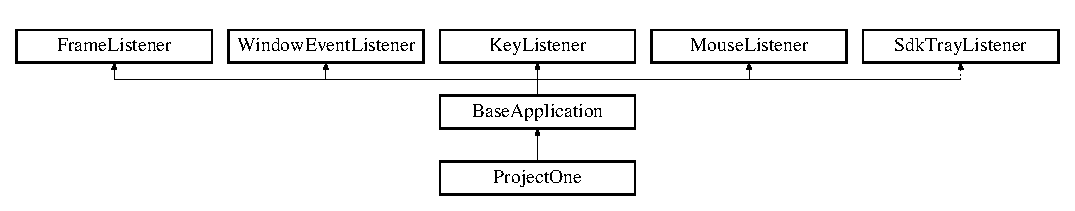
\includegraphics[height=2.382979cm]{class_base_application}
\end{center}
\end{figure}
\subsection*{Public Member Functions}
\begin{DoxyCompactItemize}
\item 
\hyperlink{class_base_application_a7c897f08816cc064568ae1ec71026719}{Base\-Application} (void)
\item 
virtual \hyperlink{class_base_application_a39133f736b9eb70263cebaca3e6d2cad}{$\sim$\-Base\-Application} (void)
\item 
virtual void \hyperlink{class_base_application_aed497661d1817ed9d659fb4de671ac1c}{go} (void)
\end{DoxyCompactItemize}
\subsection*{Public Attributes}
\begin{DoxyCompactItemize}
\item 
int \hyperlink{class_base_application_adf36bb25e5d307e0b4433489c8227b46}{main\-Tick\-Value}
\end{DoxyCompactItemize}
\subsection*{Protected Types}
\begin{DoxyCompactItemize}
\item 
enum \hyperlink{class_base_application_abc714ee35568ef8090a07419fd391ba7}{Current\-Shape\-Type} \{ \\*
\hyperlink{class_base_application_abc714ee35568ef8090a07419fd391ba7a59004bd3d877f5b50fff8444129015c4}{z\-Shape\-Type}, 
\hyperlink{class_base_application_abc714ee35568ef8090a07419fd391ba7a72677ae713741fdbf098c0c842f56a98}{box\-Type}, 
\hyperlink{class_base_application_abc714ee35568ef8090a07419fd391ba7a880f3e0a05f87a1bac9f20f4e6cbc007}{t\-Shape\-Type}, 
\hyperlink{class_base_application_abc714ee35568ef8090a07419fd391ba7a810cb2b1cc6fdb0b47584be2c47c105e}{t\-Shape\-Opp\-Type}, 
\\*
\hyperlink{class_base_application_abc714ee35568ef8090a07419fd391ba7a8b2e01912467d9c21dfdfeb53197067d}{l\-Shape\-Type}, 
\hyperlink{class_base_application_abc714ee35568ef8090a07419fd391ba7a0e9b09f1f30d29533864917d93a02ae7}{l\-Shape\-Opp\-Type}
 \}
\end{DoxyCompactItemize}
\subsection*{Protected Member Functions}
\begin{DoxyCompactItemize}
\item 
virtual bool \hyperlink{class_base_application_ae548b5e3ac0cf92d4dc7d478a8f01922}{setup} ()
\item 
virtual bool \hyperlink{class_base_application_a7882a8f2e08e8d6cde00e8c29b2153b0}{configure} (void)
\item 
virtual void \hyperlink{class_base_application_a0cf5e311b1c7426590ad6831e4c5352a}{choose\-Scene\-Manager} (void)
\item 
virtual void \hyperlink{class_base_application_ad1285286a30e44011746fe80f3bc1aa0}{create\-Camera} (void)
\item 
virtual void \hyperlink{class_base_application_ab672d2b969b8530ee753f8b000d219c6}{create\-Frame\-Listener} (void)
\item 
virtual void \hyperlink{class_base_application_aa97beeb4059b17d0ec22eae33286ec2d}{create\-Scene} (void)=0
\item 
virtual void \hyperlink{class_base_application_ab61c91a38b99f98ff369ce8098a91133}{destroy\-Scene} (void)
\item 
virtual void \hyperlink{class_base_application_a8e35ac97bd0cf7a3f90b280c8826389c}{create\-Viewports} (void)
\item 
virtual void \hyperlink{class_base_application_aa71428aeca821504352f5f795e6a9226}{setup\-Resources} (void)
\item 
virtual void \hyperlink{class_base_application_a9e916d51e4d73e355091d0662c175d85}{create\-Resource\-Listener} (void)
\item 
virtual void \hyperlink{class_base_application_a7d72de4f9e3d17ce0a4a034d780baf67}{load\-Resources} (void)
\item 
virtual bool \hyperlink{class_base_application_adea8d433b93b66ec7ab48b7e244661df}{frame\-Rendering\-Queued} (const Ogre\-::\-Frame\-Event \&evt)
\item 
virtual bool \hyperlink{class_base_application_ad79efa8c9d6f0f6a3cf8a34c25a1bd5f}{key\-Pressed} (const O\-I\-S\-::\-Key\-Event \&arg)
\item 
virtual bool \hyperlink{class_base_application_a72dbb7e590af8f96904bc55eb1875a56}{key\-Released} (const O\-I\-S\-::\-Key\-Event \&arg)
\item 
virtual bool \hyperlink{class_base_application_abbb67365fb496300701dc7a6953936fe}{mouse\-Moved} (const O\-I\-S\-::\-Mouse\-Event \&arg)
\item 
virtual bool \hyperlink{class_base_application_a51b515984916eb7a1582499ee3309ac5}{mouse\-Pressed} (const O\-I\-S\-::\-Mouse\-Event \&arg, O\-I\-S\-::\-Mouse\-Button\-I\-D id)
\item 
virtual bool \hyperlink{class_base_application_ae347f583327e4ba1eb83f2df286c1d76}{mouse\-Released} (const O\-I\-S\-::\-Mouse\-Event \&arg, O\-I\-S\-::\-Mouse\-Button\-I\-D id)
\item 
virtual void \hyperlink{class_base_application_afe5d7ca9e0f0575b4046c1412e314e69}{window\-Resized} (Ogre\-::\-Render\-Window $\ast$rw)
\item 
virtual void \hyperlink{class_base_application_aa7130c376136aa3a9b121e2dee561aed}{window\-Closed} (Ogre\-::\-Render\-Window $\ast$rw)
\item 
virtual void \hyperlink{class_base_application_a0bc96be61b7f2cc41e3b7ac416900c91}{random\-Shape} ()
\item 
void \hyperlink{class_base_application_ae2e1a92373a8ca12dcc8a9d51bb0a4cb}{create\-G\-U\-I} ()
\item 
virtual void \hyperlink{class_base_application_a67bbbb14b9643246ce747ef27cc04c45}{drop\-Level\-In3\-D\-Array} (int array\-Clear\-Height\-New)
\item 
virtual void \hyperlink{class_base_application_a344f227b3fb9c4ed73823d4f6ec8e30c}{next\-Level} ()
\item 
virtual void \hyperlink{class_base_application_a0ca8072328f7b377d1df88b8173c42cd}{check\-For\-End\-Game} ()
\end{DoxyCompactItemize}
\subsection*{Protected Attributes}
\begin{DoxyCompactItemize}
\item 
int \hyperlink{class_base_application_a1c1a812d975a0a98781314580f84c920}{array\-Clear\-Height}
\item 
int \hyperlink{class_base_application_a6a0a6b2fd0467a5d206da0a60c68b660}{array\-Height}
\item 
int \hyperlink{class_base_application_a7d8a377aa221a84cdf095927bcb48526}{array\-Width}
\item 
int \hyperlink{class_base_application_a365f02117f2afc6bc4d54aa7569cbee5}{array\-Depth}
\item 
Ogre\-::\-Log $\ast$ \hyperlink{class_base_application_a24c535ef10e1f77e477e0adc783b2245}{m\-\_\-p\-Log}
\item 
Ogre\-::\-Root $\ast$ \hyperlink{class_base_application_add84ba707dc6c57e6283f214b1274110}{m\-Root}
\item 
Ogre\-::\-Camera $\ast$ \hyperlink{class_base_application_a3829c6b12afe911e97e6b4524b33a38b}{m\-Camera}
\item 
Ogre\-::\-Scene\-Manager $\ast$ \hyperlink{class_base_application_a8a7684f4f9a57ed3089048ad1a913b2d}{m\-Scene\-Mgr}
\item 
Ogre\-::\-Render\-Window $\ast$ \hyperlink{class_base_application_ac5d8e9c81e036897bc82f81eff8c570f}{m\-Window}
\item 
Ogre\-::\-String \hyperlink{class_base_application_a765e0df01c141a16df3178ab4f17afe6}{m\-Resources\-Cfg}
\item 
Ogre\-::\-String \hyperlink{class_base_application_a04f2fe47fa164fd78d986dc0df70b7fb}{m\-Plugins\-Cfg}
\item 
Ogre\-Bites\-::\-Sdk\-Tray\-Manager $\ast$ \hyperlink{class_base_application_a7faa397f4f4861ee8c361a01e90b4416}{m\-Tray\-Mgr}
\item 
Ogre\-Bites\-::\-Sdk\-Camera\-Man $\ast$ \hyperlink{class_base_application_a9ae38dea6316058549151fff66a91fcd}{m\-Camera\-Man}
\item 
Ogre\-Bites\-::\-Params\-Panel $\ast$ \hyperlink{class_base_application_a6a11054ca61efdf558e0ff1b2de43a12}{m\-Details\-Panel}
\item 
bool \hyperlink{class_base_application_ac7e861799862cb645f1d78b170aef80d}{m\-Cursor\-Was\-Visible}
\item 
bool \hyperlink{class_base_application_a755f26d3a9915aaf830750d877e39d86}{m\-Shut\-Down}
\item 
vector$<$ vector$<$ vector$<$ \hyperlink{class_cube}{Cube} $\ast$ $>$ $>$ $>$ \hyperlink{class_base_application_a1d4876d5a2f4d69a9a0fae61ee8f5127}{array3\-D}
\item 
Gui3\-D\-::\-Gui3\-D $\ast$ \hyperlink{class_base_application_aaa51f685a5ab1f23b6152f12dbdd86a5}{m\-Gui3\-D}
\item 
Gui3\-D\-::\-Panel $\ast$ \hyperlink{class_base_application_ad367e0814cd650819f0a6b8460488f2f}{m\-Panel}
\item 
\hyperlink{struct_my_simple_demo_panel_colors}{My\-Simple\-Demo\-Panel\-Colors} \hyperlink{class_base_application_ae282cc9731cc19ae3f7c1889091c6480}{m\-My\-Simple\-Demo\-Panel\-Colors}
\item 
enum \\*
\hyperlink{class_base_application_abc714ee35568ef8090a07419fd391ba7}{Base\-Application\-::\-Current\-Shape\-Type} \hyperlink{class_base_application_ae6b860cfe7188f6c1dd32bd6fecfd2a9}{current\-Shape\-Type}
\item 
bool \hyperlink{class_base_application_abde703d00837e1f9c80698e820529a95}{used\-Z\-Shape}
\item 
bool \hyperlink{class_base_application_a97e267ce8eda15e4bec536817d9546ee}{used\-Box\-Shape}
\item 
bool \hyperlink{class_base_application_a77fa12fbd79ae12dc609b29859452e51}{used\-T\-Shape}
\item 
bool \hyperlink{class_base_application_a0997587550f66c6425a2fae78f64e2b1}{used\-T\-Shape\-Opp}
\item 
bool \hyperlink{class_base_application_a1192e80769f65e87c5cc6d7aa37d3040}{usedl\-Shape}
\item 
bool \hyperlink{class_base_application_a1617c0606b49229803b7a3ecb2d6f936}{usedl\-Shape\-Opp}
\item 
int \hyperlink{class_base_application_a9bff1519bcaf61fc3cbcc3c66ec273a3}{current\-Z\-Shape\-Cell}
\item 
int \hyperlink{class_base_application_a6cc81cb0cda55bee078cd0fe4a053a55}{current\-Box\-Shape\-Cell}
\item 
int \hyperlink{class_base_application_ae43613d0e1142a6e9b12723d5b49da1b}{current\-T\-Shape\-Cell}
\item 
int \hyperlink{class_base_application_a46497f2f8c6f6b9e34bcb7986882715f}{current\-T\-Shape\-Opp\-Cell}
\item 
int \hyperlink{class_base_application_a53b5c467e53fde6b453021bff907b26d}{currentl\-Shape\-Cell}
\item 
int \hyperlink{class_base_application_ad8dd5ed80f7ab80b4c8a88e83b251b05}{currentl\-Shape\-Opp\-Cell}
\item 
vector$<$ \hyperlink{classbox}{box} $\ast$ $>$ \hyperlink{class_base_application_ade32bf8c002709296ed8d0a789d8cbba}{boxes}
\item 
vector$<$ \hyperlink{classz_shape}{z\-Shape} $\ast$ $>$ \hyperlink{class_base_application_aa412bf0f968f597ca1ab77738eafd5f5}{z\-Shapes}
\item 
vector$<$ \hyperlink{classt_shape}{t\-Shape} $\ast$ $>$ \hyperlink{class_base_application_aec2d0eebbcdd4364649da4f412cdbb24}{t\-Shapes}
\item 
vector$<$ \hyperlink{classt_shape_opp}{t\-Shape\-Opp} $\ast$ $>$ \hyperlink{class_base_application_a38ff9c55061692b43d1d56de9bf3a363}{t\-Opp\-Shapes}
\item 
vector$<$ \hyperlink{classl_shape}{l\-Shape} $\ast$ $>$ \hyperlink{class_base_application_a064956fbdf1b5ae2c187530ec7642b68}{l\-Shapes}
\item 
vector$<$ \hyperlink{classl_shape_opp}{l\-Shape\-Opp} $\ast$ $>$ \hyperlink{class_base_application_ad4c357854ba045adac9bd2016452bb8b}{l\-Opp\-Shapes}
\item 
O\-I\-S\-::\-Input\-Manager $\ast$ \hyperlink{class_base_application_abc9503c8462e225b5d0d55c952d9e4a9}{m\-Input\-Manager}
\item 
O\-I\-S\-::\-Mouse $\ast$ \hyperlink{class_base_application_add9b97fbe64da2814d3af113bac58c43}{m\-Mouse}
\item 
O\-I\-S\-::\-Keyboard $\ast$ \hyperlink{class_base_application_a9d6e19cf50c47379fbaae55bff28079c}{m\-Keyboard}
\item 
int \hyperlink{class_base_application_a854f2a19c04bc06c187fcf5f771966cc}{layers\-Cleared}
\item 
int \hyperlink{class_base_application_abaf901b9f1c0b913235a8d818ece8772}{next\-Level\-Int}
\item 
int \hyperlink{class_base_application_a48aa9aa0d39fac2805d912b9f4e8d593}{next\-Level\-Amount}
\item 
int \hyperlink{class_base_application_a1408e82cf9d072d8b35505b7f42d8565}{current\-Level}
\item 
int \hyperlink{class_base_application_a681cfe91d2cee55f8d783651a074fdcf}{score}
\item 
int \hyperlink{class_base_application_a4484039f7dfe0e4eaa962a4fa781bc88}{score\-Multiplier}
\item 
Ogre\-::\-Timer \hyperlink{class_base_application_a7e2bb2cec7b0185bf861d5bf5f8c015c}{\-\_\-timer}
\item 
bool \hyperlink{class_base_application_a3cd36d39f168b56476c22d27cf9cb429}{music}
\item 
bool \hyperlink{class_base_application_a4a21a832334bce0266af82d97208c5d1}{effects}
\item 
bool \hyperlink{class_base_application_adadae473e6c936a899153c205c2de07d}{init}
\item 
int \hyperlink{class_base_application_aad18724507e497250a90dd9d12d24920}{timer\-C\-H\-E\-C\-K}
\item 
F\-M\-O\-D\-::\-System $\ast$ \hyperlink{class_base_application_ac45b5d8be5f852e28d13b2009c45b5a5}{F\-M\-O\-Dsys}
\item 
F\-M\-O\-D\-\_\-\-R\-E\-S\-U\-L\-T \hyperlink{class_base_application_ad50a268c7b77ee4e910eca0d96430705}{result}
\item 
F\-M\-O\-D\-::\-Sound $\ast$ \hyperlink{class_base_application_aea4ddf4bf2fe2f475e75ac1754e64b0c}{sound}
\item 
F\-M\-O\-D\-::\-Sound $\ast$ \hyperlink{class_base_application_ac1cb587fccc3d6d0a263d484bc6829bc}{sound\-Start}
\item 
F\-M\-O\-D\-::\-Sound $\ast$ \hyperlink{class_base_application_aab866d736fb7032813be4f0692bf40a6}{sound\-Drop}
\item 
F\-M\-O\-D\-::\-Channel $\ast$ \hyperlink{class_base_application_ab6938e41749182bbe867f455ad52cf09}{channel}
\item 
F\-M\-O\-D\-::\-Channel $\ast$ \hyperlink{class_base_application_aceea4286991e9718baa4278671d8c836}{channel2}
\item 
F\-M\-O\-D\-::\-Channel $\ast$ \hyperlink{class_base_application_adfa511eb6241720fc95c1c32f92deb80}{channel3}
\item 
F\-M\-O\-D\-::\-Reverb $\ast$ \hyperlink{class_base_application_a92820c32798f0d3928fcce24787eda1f}{reverb}
\item 
F\-M\-O\-D\-::\-Reverb $\ast$ \hyperlink{class_base_application_a1b0ab0994f1beef254a3020b5b2a0945}{reverb2}
\end{DoxyCompactItemize}


\subsection{Member Enumeration Documentation}
\hypertarget{class_base_application_abc714ee35568ef8090a07419fd391ba7}{\index{Base\-Application@{Base\-Application}!Current\-Shape\-Type@{Current\-Shape\-Type}}
\index{Current\-Shape\-Type@{Current\-Shape\-Type}!BaseApplication@{Base\-Application}}
\subsubsection[{Current\-Shape\-Type}]{\setlength{\rightskip}{0pt plus 5cm}enum {\bf Base\-Application\-::\-Current\-Shape\-Type}\hspace{0.3cm}{\ttfamily [protected]}}}\label{class_base_application_abc714ee35568ef8090a07419fd391ba7}
an enumeration used to indicate what the current shape type being used by the player is \begin{Desc}
\item[Enumerator]\par
\begin{description}
\index{z\-Shape\-Type@{z\-Shape\-Type}!Base\-Application@{Base\-Application}}\index{Base\-Application@{Base\-Application}!z\-Shape\-Type@{z\-Shape\-Type}}\item[{\em 
\hypertarget{class_base_application_abc714ee35568ef8090a07419fd391ba7a59004bd3d877f5b50fff8444129015c4}{z\-Shape\-Type}\label{class_base_application_abc714ee35568ef8090a07419fd391ba7a59004bd3d877f5b50fff8444129015c4}
}]\index{box\-Type@{box\-Type}!Base\-Application@{Base\-Application}}\index{Base\-Application@{Base\-Application}!box\-Type@{box\-Type}}\item[{\em 
\hypertarget{class_base_application_abc714ee35568ef8090a07419fd391ba7a72677ae713741fdbf098c0c842f56a98}{box\-Type}\label{class_base_application_abc714ee35568ef8090a07419fd391ba7a72677ae713741fdbf098c0c842f56a98}
}]\index{t\-Shape\-Type@{t\-Shape\-Type}!Base\-Application@{Base\-Application}}\index{Base\-Application@{Base\-Application}!t\-Shape\-Type@{t\-Shape\-Type}}\item[{\em 
\hypertarget{class_base_application_abc714ee35568ef8090a07419fd391ba7a880f3e0a05f87a1bac9f20f4e6cbc007}{t\-Shape\-Type}\label{class_base_application_abc714ee35568ef8090a07419fd391ba7a880f3e0a05f87a1bac9f20f4e6cbc007}
}]\index{t\-Shape\-Opp\-Type@{t\-Shape\-Opp\-Type}!Base\-Application@{Base\-Application}}\index{Base\-Application@{Base\-Application}!t\-Shape\-Opp\-Type@{t\-Shape\-Opp\-Type}}\item[{\em 
\hypertarget{class_base_application_abc714ee35568ef8090a07419fd391ba7a810cb2b1cc6fdb0b47584be2c47c105e}{t\-Shape\-Opp\-Type}\label{class_base_application_abc714ee35568ef8090a07419fd391ba7a810cb2b1cc6fdb0b47584be2c47c105e}
}]\index{l\-Shape\-Type@{l\-Shape\-Type}!Base\-Application@{Base\-Application}}\index{Base\-Application@{Base\-Application}!l\-Shape\-Type@{l\-Shape\-Type}}\item[{\em 
\hypertarget{class_base_application_abc714ee35568ef8090a07419fd391ba7a8b2e01912467d9c21dfdfeb53197067d}{l\-Shape\-Type}\label{class_base_application_abc714ee35568ef8090a07419fd391ba7a8b2e01912467d9c21dfdfeb53197067d}
}]\index{l\-Shape\-Opp\-Type@{l\-Shape\-Opp\-Type}!Base\-Application@{Base\-Application}}\index{Base\-Application@{Base\-Application}!l\-Shape\-Opp\-Type@{l\-Shape\-Opp\-Type}}\item[{\em 
\hypertarget{class_base_application_abc714ee35568ef8090a07419fd391ba7a0e9b09f1f30d29533864917d93a02ae7}{l\-Shape\-Opp\-Type}\label{class_base_application_abc714ee35568ef8090a07419fd391ba7a0e9b09f1f30d29533864917d93a02ae7}
}]\end{description}
\end{Desc}


\subsection{Constructor \& Destructor Documentation}
\hypertarget{class_base_application_a7c897f08816cc064568ae1ec71026719}{\index{Base\-Application@{Base\-Application}!Base\-Application@{Base\-Application}}
\index{Base\-Application@{Base\-Application}!BaseApplication@{Base\-Application}}
\subsubsection[{Base\-Application}]{\setlength{\rightskip}{0pt plus 5cm}Base\-Application\-::\-Base\-Application (
\begin{DoxyParamCaption}
\item[{void}]{}
\end{DoxyParamCaption}
)}}\label{class_base_application_a7c897f08816cc064568ae1ec71026719}
\hypertarget{class_base_application_a39133f736b9eb70263cebaca3e6d2cad}{\index{Base\-Application@{Base\-Application}!$\sim$\-Base\-Application@{$\sim$\-Base\-Application}}
\index{$\sim$\-Base\-Application@{$\sim$\-Base\-Application}!BaseApplication@{Base\-Application}}
\subsubsection[{$\sim$\-Base\-Application}]{\setlength{\rightskip}{0pt plus 5cm}virtual Base\-Application\-::$\sim$\-Base\-Application (
\begin{DoxyParamCaption}
\item[{void}]{}
\end{DoxyParamCaption}
)\hspace{0.3cm}{\ttfamily [virtual]}}}\label{class_base_application_a39133f736b9eb70263cebaca3e6d2cad}


\subsection{Member Function Documentation}
\hypertarget{class_base_application_a0ca8072328f7b377d1df88b8173c42cd}{\index{Base\-Application@{Base\-Application}!check\-For\-End\-Game@{check\-For\-End\-Game}}
\index{check\-For\-End\-Game@{check\-For\-End\-Game}!BaseApplication@{Base\-Application}}
\subsubsection[{check\-For\-End\-Game}]{\setlength{\rightskip}{0pt plus 5cm}virtual void Base\-Application\-::check\-For\-End\-Game (
\begin{DoxyParamCaption}
{}
\end{DoxyParamCaption}
)\hspace{0.3cm}{\ttfamily [protected]}, {\ttfamily [virtual]}}}\label{class_base_application_a0ca8072328f7b377d1df88b8173c42cd}
This method checks if the cells above the array are empty and if not it ends the game \hypertarget{class_base_application_a0cf5e311b1c7426590ad6831e4c5352a}{\index{Base\-Application@{Base\-Application}!choose\-Scene\-Manager@{choose\-Scene\-Manager}}
\index{choose\-Scene\-Manager@{choose\-Scene\-Manager}!BaseApplication@{Base\-Application}}
\subsubsection[{choose\-Scene\-Manager}]{\setlength{\rightskip}{0pt plus 5cm}virtual void Base\-Application\-::choose\-Scene\-Manager (
\begin{DoxyParamCaption}
\item[{void}]{}
\end{DoxyParamCaption}
)\hspace{0.3cm}{\ttfamily [protected]}, {\ttfamily [virtual]}}}\label{class_base_application_a0cf5e311b1c7426590ad6831e4c5352a}
\hypertarget{class_base_application_a7882a8f2e08e8d6cde00e8c29b2153b0}{\index{Base\-Application@{Base\-Application}!configure@{configure}}
\index{configure@{configure}!BaseApplication@{Base\-Application}}
\subsubsection[{configure}]{\setlength{\rightskip}{0pt plus 5cm}virtual bool Base\-Application\-::configure (
\begin{DoxyParamCaption}
\item[{void}]{}
\end{DoxyParamCaption}
)\hspace{0.3cm}{\ttfamily [protected]}, {\ttfamily [virtual]}}}\label{class_base_application_a7882a8f2e08e8d6cde00e8c29b2153b0}
\hypertarget{class_base_application_ad1285286a30e44011746fe80f3bc1aa0}{\index{Base\-Application@{Base\-Application}!create\-Camera@{create\-Camera}}
\index{create\-Camera@{create\-Camera}!BaseApplication@{Base\-Application}}
\subsubsection[{create\-Camera}]{\setlength{\rightskip}{0pt plus 5cm}virtual void Base\-Application\-::create\-Camera (
\begin{DoxyParamCaption}
\item[{void}]{}
\end{DoxyParamCaption}
)\hspace{0.3cm}{\ttfamily [protected]}, {\ttfamily [virtual]}}}\label{class_base_application_ad1285286a30e44011746fe80f3bc1aa0}
\hypertarget{class_base_application_ab672d2b969b8530ee753f8b000d219c6}{\index{Base\-Application@{Base\-Application}!create\-Frame\-Listener@{create\-Frame\-Listener}}
\index{create\-Frame\-Listener@{create\-Frame\-Listener}!BaseApplication@{Base\-Application}}
\subsubsection[{create\-Frame\-Listener}]{\setlength{\rightskip}{0pt plus 5cm}virtual void Base\-Application\-::create\-Frame\-Listener (
\begin{DoxyParamCaption}
\item[{void}]{}
\end{DoxyParamCaption}
)\hspace{0.3cm}{\ttfamily [protected]}, {\ttfamily [virtual]}}}\label{class_base_application_ab672d2b969b8530ee753f8b000d219c6}
\hypertarget{class_base_application_ae2e1a92373a8ca12dcc8a9d51bb0a4cb}{\index{Base\-Application@{Base\-Application}!create\-G\-U\-I@{create\-G\-U\-I}}
\index{create\-G\-U\-I@{create\-G\-U\-I}!BaseApplication@{Base\-Application}}
\subsubsection[{create\-G\-U\-I}]{\setlength{\rightskip}{0pt plus 5cm}void Base\-Application\-::create\-G\-U\-I (
\begin{DoxyParamCaption}
{}
\end{DoxyParamCaption}
)\hspace{0.3cm}{\ttfamily [protected]}}}\label{class_base_application_ae2e1a92373a8ca12dcc8a9d51bb0a4cb}
creates the G\-U\-I interface \hypertarget{class_base_application_a9e916d51e4d73e355091d0662c175d85}{\index{Base\-Application@{Base\-Application}!create\-Resource\-Listener@{create\-Resource\-Listener}}
\index{create\-Resource\-Listener@{create\-Resource\-Listener}!BaseApplication@{Base\-Application}}
\subsubsection[{create\-Resource\-Listener}]{\setlength{\rightskip}{0pt plus 5cm}virtual void Base\-Application\-::create\-Resource\-Listener (
\begin{DoxyParamCaption}
\item[{void}]{}
\end{DoxyParamCaption}
)\hspace{0.3cm}{\ttfamily [protected]}, {\ttfamily [virtual]}}}\label{class_base_application_a9e916d51e4d73e355091d0662c175d85}
\hypertarget{class_base_application_aa97beeb4059b17d0ec22eae33286ec2d}{\index{Base\-Application@{Base\-Application}!create\-Scene@{create\-Scene}}
\index{create\-Scene@{create\-Scene}!BaseApplication@{Base\-Application}}
\subsubsection[{create\-Scene}]{\setlength{\rightskip}{0pt plus 5cm}virtual void Base\-Application\-::create\-Scene (
\begin{DoxyParamCaption}
\item[{void}]{}
\end{DoxyParamCaption}
)\hspace{0.3cm}{\ttfamily [protected]}, {\ttfamily [pure virtual]}}}\label{class_base_application_aa97beeb4059b17d0ec22eae33286ec2d}


Implemented in \hyperlink{class_project_one_a61b71d677e7e4e3ac80071431b65ca5c}{Project\-One}.

\hypertarget{class_base_application_a8e35ac97bd0cf7a3f90b280c8826389c}{\index{Base\-Application@{Base\-Application}!create\-Viewports@{create\-Viewports}}
\index{create\-Viewports@{create\-Viewports}!BaseApplication@{Base\-Application}}
\subsubsection[{create\-Viewports}]{\setlength{\rightskip}{0pt plus 5cm}virtual void Base\-Application\-::create\-Viewports (
\begin{DoxyParamCaption}
\item[{void}]{}
\end{DoxyParamCaption}
)\hspace{0.3cm}{\ttfamily [protected]}, {\ttfamily [virtual]}}}\label{class_base_application_a8e35ac97bd0cf7a3f90b280c8826389c}
\hypertarget{class_base_application_ab61c91a38b99f98ff369ce8098a91133}{\index{Base\-Application@{Base\-Application}!destroy\-Scene@{destroy\-Scene}}
\index{destroy\-Scene@{destroy\-Scene}!BaseApplication@{Base\-Application}}
\subsubsection[{destroy\-Scene}]{\setlength{\rightskip}{0pt plus 5cm}virtual void Base\-Application\-::destroy\-Scene (
\begin{DoxyParamCaption}
\item[{void}]{}
\end{DoxyParamCaption}
)\hspace{0.3cm}{\ttfamily [protected]}, {\ttfamily [virtual]}}}\label{class_base_application_ab61c91a38b99f98ff369ce8098a91133}
\hypertarget{class_base_application_a67bbbb14b9643246ce747ef27cc04c45}{\index{Base\-Application@{Base\-Application}!drop\-Level\-In3\-D\-Array@{drop\-Level\-In3\-D\-Array}}
\index{drop\-Level\-In3\-D\-Array@{drop\-Level\-In3\-D\-Array}!BaseApplication@{Base\-Application}}
\subsubsection[{drop\-Level\-In3\-D\-Array}]{\setlength{\rightskip}{0pt plus 5cm}virtual void Base\-Application\-::drop\-Level\-In3\-D\-Array (
\begin{DoxyParamCaption}
\item[{int}]{array\-Clear\-Height\-New}
\end{DoxyParamCaption}
)\hspace{0.3cm}{\ttfamily [protected]}, {\ttfamily [virtual]}}}\label{class_base_application_a67bbbb14b9643246ce747ef27cc04c45}
This method goes through the 3\-D array starting from the clear\-Height and moves each cell above the height down one in the y-\/direction (if the cell is not null) \hypertarget{class_base_application_adea8d433b93b66ec7ab48b7e244661df}{\index{Base\-Application@{Base\-Application}!frame\-Rendering\-Queued@{frame\-Rendering\-Queued}}
\index{frame\-Rendering\-Queued@{frame\-Rendering\-Queued}!BaseApplication@{Base\-Application}}
\subsubsection[{frame\-Rendering\-Queued}]{\setlength{\rightskip}{0pt plus 5cm}virtual bool Base\-Application\-::frame\-Rendering\-Queued (
\begin{DoxyParamCaption}
\item[{const Ogre\-::\-Frame\-Event \&}]{evt}
\end{DoxyParamCaption}
)\hspace{0.3cm}{\ttfamily [protected]}, {\ttfamily [virtual]}}}\label{class_base_application_adea8d433b93b66ec7ab48b7e244661df}
Ogre\-::\-Frame\-Listener \hypertarget{class_base_application_aed497661d1817ed9d659fb4de671ac1c}{\index{Base\-Application@{Base\-Application}!go@{go}}
\index{go@{go}!BaseApplication@{Base\-Application}}
\subsubsection[{go}]{\setlength{\rightskip}{0pt plus 5cm}virtual void Base\-Application\-::go (
\begin{DoxyParamCaption}
\item[{void}]{}
\end{DoxyParamCaption}
)\hspace{0.3cm}{\ttfamily [virtual]}}}\label{class_base_application_aed497661d1817ed9d659fb4de671ac1c}
\hypertarget{class_base_application_ad79efa8c9d6f0f6a3cf8a34c25a1bd5f}{\index{Base\-Application@{Base\-Application}!key\-Pressed@{key\-Pressed}}
\index{key\-Pressed@{key\-Pressed}!BaseApplication@{Base\-Application}}
\subsubsection[{key\-Pressed}]{\setlength{\rightskip}{0pt plus 5cm}virtual bool Base\-Application\-::key\-Pressed (
\begin{DoxyParamCaption}
\item[{const O\-I\-S\-::\-Key\-Event \&}]{arg}
\end{DoxyParamCaption}
)\hspace{0.3cm}{\ttfamily [protected]}, {\ttfamily [virtual]}}}\label{class_base_application_ad79efa8c9d6f0f6a3cf8a34c25a1bd5f}
O\-I\-S\-::\-Key\-Listener \hypertarget{class_base_application_a72dbb7e590af8f96904bc55eb1875a56}{\index{Base\-Application@{Base\-Application}!key\-Released@{key\-Released}}
\index{key\-Released@{key\-Released}!BaseApplication@{Base\-Application}}
\subsubsection[{key\-Released}]{\setlength{\rightskip}{0pt plus 5cm}virtual bool Base\-Application\-::key\-Released (
\begin{DoxyParamCaption}
\item[{const O\-I\-S\-::\-Key\-Event \&}]{arg}
\end{DoxyParamCaption}
)\hspace{0.3cm}{\ttfamily [protected]}, {\ttfamily [virtual]}}}\label{class_base_application_a72dbb7e590af8f96904bc55eb1875a56}
\hypertarget{class_base_application_a7d72de4f9e3d17ce0a4a034d780baf67}{\index{Base\-Application@{Base\-Application}!load\-Resources@{load\-Resources}}
\index{load\-Resources@{load\-Resources}!BaseApplication@{Base\-Application}}
\subsubsection[{load\-Resources}]{\setlength{\rightskip}{0pt plus 5cm}virtual void Base\-Application\-::load\-Resources (
\begin{DoxyParamCaption}
\item[{void}]{}
\end{DoxyParamCaption}
)\hspace{0.3cm}{\ttfamily [protected]}, {\ttfamily [virtual]}}}\label{class_base_application_a7d72de4f9e3d17ce0a4a034d780baf67}
\hypertarget{class_base_application_abbb67365fb496300701dc7a6953936fe}{\index{Base\-Application@{Base\-Application}!mouse\-Moved@{mouse\-Moved}}
\index{mouse\-Moved@{mouse\-Moved}!BaseApplication@{Base\-Application}}
\subsubsection[{mouse\-Moved}]{\setlength{\rightskip}{0pt plus 5cm}virtual bool Base\-Application\-::mouse\-Moved (
\begin{DoxyParamCaption}
\item[{const O\-I\-S\-::\-Mouse\-Event \&}]{arg}
\end{DoxyParamCaption}
)\hspace{0.3cm}{\ttfamily [protected]}, {\ttfamily [virtual]}}}\label{class_base_application_abbb67365fb496300701dc7a6953936fe}
O\-I\-S\-::\-Mouse\-Listener \hypertarget{class_base_application_a51b515984916eb7a1582499ee3309ac5}{\index{Base\-Application@{Base\-Application}!mouse\-Pressed@{mouse\-Pressed}}
\index{mouse\-Pressed@{mouse\-Pressed}!BaseApplication@{Base\-Application}}
\subsubsection[{mouse\-Pressed}]{\setlength{\rightskip}{0pt plus 5cm}virtual bool Base\-Application\-::mouse\-Pressed (
\begin{DoxyParamCaption}
\item[{const O\-I\-S\-::\-Mouse\-Event \&}]{arg, }
\item[{O\-I\-S\-::\-Mouse\-Button\-I\-D}]{id}
\end{DoxyParamCaption}
)\hspace{0.3cm}{\ttfamily [protected]}, {\ttfamily [virtual]}}}\label{class_base_application_a51b515984916eb7a1582499ee3309ac5}
\hypertarget{class_base_application_ae347f583327e4ba1eb83f2df286c1d76}{\index{Base\-Application@{Base\-Application}!mouse\-Released@{mouse\-Released}}
\index{mouse\-Released@{mouse\-Released}!BaseApplication@{Base\-Application}}
\subsubsection[{mouse\-Released}]{\setlength{\rightskip}{0pt plus 5cm}virtual bool Base\-Application\-::mouse\-Released (
\begin{DoxyParamCaption}
\item[{const O\-I\-S\-::\-Mouse\-Event \&}]{arg, }
\item[{O\-I\-S\-::\-Mouse\-Button\-I\-D}]{id}
\end{DoxyParamCaption}
)\hspace{0.3cm}{\ttfamily [protected]}, {\ttfamily [virtual]}}}\label{class_base_application_ae347f583327e4ba1eb83f2df286c1d76}
\hypertarget{class_base_application_a344f227b3fb9c4ed73823d4f6ec8e30c}{\index{Base\-Application@{Base\-Application}!next\-Level@{next\-Level}}
\index{next\-Level@{next\-Level}!BaseApplication@{Base\-Application}}
\subsubsection[{next\-Level}]{\setlength{\rightskip}{0pt plus 5cm}virtual void Base\-Application\-::next\-Level (
\begin{DoxyParamCaption}
{}
\end{DoxyParamCaption}
)\hspace{0.3cm}{\ttfamily [protected]}, {\ttfamily [virtual]}}}\label{class_base_application_a344f227b3fb9c4ed73823d4f6ec8e30c}
This method iterates up a level to the next level \hypertarget{class_base_application_a0bc96be61b7f2cc41e3b7ac416900c91}{\index{Base\-Application@{Base\-Application}!random\-Shape@{random\-Shape}}
\index{random\-Shape@{random\-Shape}!BaseApplication@{Base\-Application}}
\subsubsection[{random\-Shape}]{\setlength{\rightskip}{0pt plus 5cm}virtual void Base\-Application\-::random\-Shape (
\begin{DoxyParamCaption}
{}
\end{DoxyParamCaption}
)\hspace{0.3cm}{\ttfamily [protected]}, {\ttfamily [virtual]}}}\label{class_base_application_a0bc96be61b7f2cc41e3b7ac416900c91}
This method gets a random shape from an option of 6 and then sets a bool to true to say that shape has been used, This is an adaptation of the 7 bag algorithm used in tetris the shape cannot be used again until all shapes bools have been set to true (This creates semi-\/randomly generated shapes as completely random would make the game unplayable) \hypertarget{class_base_application_ae548b5e3ac0cf92d4dc7d478a8f01922}{\index{Base\-Application@{Base\-Application}!setup@{setup}}
\index{setup@{setup}!BaseApplication@{Base\-Application}}
\subsubsection[{setup}]{\setlength{\rightskip}{0pt plus 5cm}virtual bool Base\-Application\-::setup (
\begin{DoxyParamCaption}
{}
\end{DoxyParamCaption}
)\hspace{0.3cm}{\ttfamily [protected]}, {\ttfamily [virtual]}}}\label{class_base_application_ae548b5e3ac0cf92d4dc7d478a8f01922}
\hypertarget{class_base_application_aa71428aeca821504352f5f795e6a9226}{\index{Base\-Application@{Base\-Application}!setup\-Resources@{setup\-Resources}}
\index{setup\-Resources@{setup\-Resources}!BaseApplication@{Base\-Application}}
\subsubsection[{setup\-Resources}]{\setlength{\rightskip}{0pt plus 5cm}virtual void Base\-Application\-::setup\-Resources (
\begin{DoxyParamCaption}
\item[{void}]{}
\end{DoxyParamCaption}
)\hspace{0.3cm}{\ttfamily [protected]}, {\ttfamily [virtual]}}}\label{class_base_application_aa71428aeca821504352f5f795e6a9226}
\hypertarget{class_base_application_aa7130c376136aa3a9b121e2dee561aed}{\index{Base\-Application@{Base\-Application}!window\-Closed@{window\-Closed}}
\index{window\-Closed@{window\-Closed}!BaseApplication@{Base\-Application}}
\subsubsection[{window\-Closed}]{\setlength{\rightskip}{0pt plus 5cm}virtual void Base\-Application\-::window\-Closed (
\begin{DoxyParamCaption}
\item[{Ogre\-::\-Render\-Window $\ast$}]{rw}
\end{DoxyParamCaption}
)\hspace{0.3cm}{\ttfamily [protected]}, {\ttfamily [virtual]}}}\label{class_base_application_aa7130c376136aa3a9b121e2dee561aed}
\hypertarget{class_base_application_afe5d7ca9e0f0575b4046c1412e314e69}{\index{Base\-Application@{Base\-Application}!window\-Resized@{window\-Resized}}
\index{window\-Resized@{window\-Resized}!BaseApplication@{Base\-Application}}
\subsubsection[{window\-Resized}]{\setlength{\rightskip}{0pt plus 5cm}virtual void Base\-Application\-::window\-Resized (
\begin{DoxyParamCaption}
\item[{Ogre\-::\-Render\-Window $\ast$}]{rw}
\end{DoxyParamCaption}
)\hspace{0.3cm}{\ttfamily [protected]}, {\ttfamily [virtual]}}}\label{class_base_application_afe5d7ca9e0f0575b4046c1412e314e69}
Ogre\-::\-Window\-Event\-Listener 

\subsection{Member Data Documentation}
\hypertarget{class_base_application_a7e2bb2cec7b0185bf861d5bf5f8c015c}{\index{Base\-Application@{Base\-Application}!\-\_\-timer@{\-\_\-timer}}
\index{\-\_\-timer@{\-\_\-timer}!BaseApplication@{Base\-Application}}
\subsubsection[{\-\_\-timer}]{\setlength{\rightskip}{0pt plus 5cm}Ogre\-::\-Timer Base\-Application\-::\-\_\-timer\hspace{0.3cm}{\ttfamily [protected]}}}\label{class_base_application_a7e2bb2cec7b0185bf861d5bf5f8c015c}
timer \hypertarget{class_base_application_a1d4876d5a2f4d69a9a0fae61ee8f5127}{\index{Base\-Application@{Base\-Application}!array3\-D@{array3\-D}}
\index{array3\-D@{array3\-D}!BaseApplication@{Base\-Application}}
\subsubsection[{array3\-D}]{\setlength{\rightskip}{0pt plus 5cm}vector$<$vector$<$vector$<${\bf Cube}$\ast$$>$ $>$ $>$ Base\-Application\-::array3\-D\hspace{0.3cm}{\ttfamily [protected]}}}\label{class_base_application_a1d4876d5a2f4d69a9a0fae61ee8f5127}
(the grid) an empty 3\-D array of cubes used to store pointers to cubes as shapes drop into place into the grid constantly changed and updated with new positions \hypertarget{class_base_application_a1c1a812d975a0a98781314580f84c920}{\index{Base\-Application@{Base\-Application}!array\-Clear\-Height@{array\-Clear\-Height}}
\index{array\-Clear\-Height@{array\-Clear\-Height}!BaseApplication@{Base\-Application}}
\subsubsection[{array\-Clear\-Height}]{\setlength{\rightskip}{0pt plus 5cm}int Base\-Application\-::array\-Clear\-Height\hspace{0.3cm}{\ttfamily [protected]}}}\label{class_base_application_a1c1a812d975a0a98781314580f84c920}
integer used to indicate what height a layer has been cleared from the 3\-D Array \hypertarget{class_base_application_a365f02117f2afc6bc4d54aa7569cbee5}{\index{Base\-Application@{Base\-Application}!array\-Depth@{array\-Depth}}
\index{array\-Depth@{array\-Depth}!BaseApplication@{Base\-Application}}
\subsubsection[{array\-Depth}]{\setlength{\rightskip}{0pt plus 5cm}int Base\-Application\-::array\-Depth\hspace{0.3cm}{\ttfamily [protected]}}}\label{class_base_application_a365f02117f2afc6bc4d54aa7569cbee5}
integer used to store the array depth \hypertarget{class_base_application_a6a0a6b2fd0467a5d206da0a60c68b660}{\index{Base\-Application@{Base\-Application}!array\-Height@{array\-Height}}
\index{array\-Height@{array\-Height}!BaseApplication@{Base\-Application}}
\subsubsection[{array\-Height}]{\setlength{\rightskip}{0pt plus 5cm}int Base\-Application\-::array\-Height\hspace{0.3cm}{\ttfamily [protected]}}}\label{class_base_application_a6a0a6b2fd0467a5d206da0a60c68b660}
integer used to store the array height \hypertarget{class_base_application_a7d8a377aa221a84cdf095927bcb48526}{\index{Base\-Application@{Base\-Application}!array\-Width@{array\-Width}}
\index{array\-Width@{array\-Width}!BaseApplication@{Base\-Application}}
\subsubsection[{array\-Width}]{\setlength{\rightskip}{0pt plus 5cm}int Base\-Application\-::array\-Width\hspace{0.3cm}{\ttfamily [protected]}}}\label{class_base_application_a7d8a377aa221a84cdf095927bcb48526}
integer used to store the array width \hypertarget{class_base_application_ade32bf8c002709296ed8d0a789d8cbba}{\index{Base\-Application@{Base\-Application}!boxes@{boxes}}
\index{boxes@{boxes}!BaseApplication@{Base\-Application}}
\subsubsection[{boxes}]{\setlength{\rightskip}{0pt plus 5cm}vector$<${\bf box}$\ast$$>$ Base\-Application\-::boxes\hspace{0.3cm}{\ttfamily [protected]}}}\label{class_base_application_ade32bf8c002709296ed8d0a789d8cbba}
vector containers used to store each type of shape and to allow for many instances of each shape ( I considered using a heterogenous container but decided not to) (also I know that there is a memory leak as I do not currently delete shapes in the cells that are not shown during gameplay \hypertarget{class_base_application_ab6938e41749182bbe867f455ad52cf09}{\index{Base\-Application@{Base\-Application}!channel@{channel}}
\index{channel@{channel}!BaseApplication@{Base\-Application}}
\subsubsection[{channel}]{\setlength{\rightskip}{0pt plus 5cm}F\-M\-O\-D\-::\-Channel$\ast$ Base\-Application\-::channel\hspace{0.3cm}{\ttfamily [protected]}}}\label{class_base_application_ab6938e41749182bbe867f455ad52cf09}
\hypertarget{class_base_application_aceea4286991e9718baa4278671d8c836}{\index{Base\-Application@{Base\-Application}!channel2@{channel2}}
\index{channel2@{channel2}!BaseApplication@{Base\-Application}}
\subsubsection[{channel2}]{\setlength{\rightskip}{0pt plus 5cm}F\-M\-O\-D\-::\-Channel$\ast$ Base\-Application\-::channel2\hspace{0.3cm}{\ttfamily [protected]}}}\label{class_base_application_aceea4286991e9718baa4278671d8c836}
\hypertarget{class_base_application_adfa511eb6241720fc95c1c32f92deb80}{\index{Base\-Application@{Base\-Application}!channel3@{channel3}}
\index{channel3@{channel3}!BaseApplication@{Base\-Application}}
\subsubsection[{channel3}]{\setlength{\rightskip}{0pt plus 5cm}F\-M\-O\-D\-::\-Channel$\ast$ Base\-Application\-::channel3\hspace{0.3cm}{\ttfamily [protected]}}}\label{class_base_application_adfa511eb6241720fc95c1c32f92deb80}
\hypertarget{class_base_application_a6cc81cb0cda55bee078cd0fe4a053a55}{\index{Base\-Application@{Base\-Application}!current\-Box\-Shape\-Cell@{current\-Box\-Shape\-Cell}}
\index{current\-Box\-Shape\-Cell@{current\-Box\-Shape\-Cell}!BaseApplication@{Base\-Application}}
\subsubsection[{current\-Box\-Shape\-Cell}]{\setlength{\rightskip}{0pt plus 5cm}int Base\-Application\-::current\-Box\-Shape\-Cell\hspace{0.3cm}{\ttfamily [protected]}}}\label{class_base_application_a6cc81cb0cda55bee078cd0fe4a053a55}
\hypertarget{class_base_application_a1408e82cf9d072d8b35505b7f42d8565}{\index{Base\-Application@{Base\-Application}!current\-Level@{current\-Level}}
\index{current\-Level@{current\-Level}!BaseApplication@{Base\-Application}}
\subsubsection[{current\-Level}]{\setlength{\rightskip}{0pt plus 5cm}int Base\-Application\-::current\-Level\hspace{0.3cm}{\ttfamily [protected]}}}\label{class_base_application_a1408e82cf9d072d8b35505b7f42d8565}
The current level \hypertarget{class_base_application_a53b5c467e53fde6b453021bff907b26d}{\index{Base\-Application@{Base\-Application}!currentl\-Shape\-Cell@{currentl\-Shape\-Cell}}
\index{currentl\-Shape\-Cell@{currentl\-Shape\-Cell}!BaseApplication@{Base\-Application}}
\subsubsection[{currentl\-Shape\-Cell}]{\setlength{\rightskip}{0pt plus 5cm}int Base\-Application\-::currentl\-Shape\-Cell\hspace{0.3cm}{\ttfamily [protected]}}}\label{class_base_application_a53b5c467e53fde6b453021bff907b26d}
\hypertarget{class_base_application_ad8dd5ed80f7ab80b4c8a88e83b251b05}{\index{Base\-Application@{Base\-Application}!currentl\-Shape\-Opp\-Cell@{currentl\-Shape\-Opp\-Cell}}
\index{currentl\-Shape\-Opp\-Cell@{currentl\-Shape\-Opp\-Cell}!BaseApplication@{Base\-Application}}
\subsubsection[{currentl\-Shape\-Opp\-Cell}]{\setlength{\rightskip}{0pt plus 5cm}int Base\-Application\-::currentl\-Shape\-Opp\-Cell\hspace{0.3cm}{\ttfamily [protected]}}}\label{class_base_application_ad8dd5ed80f7ab80b4c8a88e83b251b05}
\hypertarget{class_base_application_ae6b860cfe7188f6c1dd32bd6fecfd2a9}{\index{Base\-Application@{Base\-Application}!current\-Shape\-Type@{current\-Shape\-Type}}
\index{current\-Shape\-Type@{current\-Shape\-Type}!BaseApplication@{Base\-Application}}
\subsubsection[{current\-Shape\-Type}]{\setlength{\rightskip}{0pt plus 5cm}enum {\bf Base\-Application\-::\-Current\-Shape\-Type}  Base\-Application\-::current\-Shape\-Type\hspace{0.3cm}{\ttfamily [protected]}}}\label{class_base_application_ae6b860cfe7188f6c1dd32bd6fecfd2a9}
\hypertarget{class_base_application_ae43613d0e1142a6e9b12723d5b49da1b}{\index{Base\-Application@{Base\-Application}!current\-T\-Shape\-Cell@{current\-T\-Shape\-Cell}}
\index{current\-T\-Shape\-Cell@{current\-T\-Shape\-Cell}!BaseApplication@{Base\-Application}}
\subsubsection[{current\-T\-Shape\-Cell}]{\setlength{\rightskip}{0pt plus 5cm}int Base\-Application\-::current\-T\-Shape\-Cell\hspace{0.3cm}{\ttfamily [protected]}}}\label{class_base_application_ae43613d0e1142a6e9b12723d5b49da1b}
\hypertarget{class_base_application_a46497f2f8c6f6b9e34bcb7986882715f}{\index{Base\-Application@{Base\-Application}!current\-T\-Shape\-Opp\-Cell@{current\-T\-Shape\-Opp\-Cell}}
\index{current\-T\-Shape\-Opp\-Cell@{current\-T\-Shape\-Opp\-Cell}!BaseApplication@{Base\-Application}}
\subsubsection[{current\-T\-Shape\-Opp\-Cell}]{\setlength{\rightskip}{0pt plus 5cm}int Base\-Application\-::current\-T\-Shape\-Opp\-Cell\hspace{0.3cm}{\ttfamily [protected]}}}\label{class_base_application_a46497f2f8c6f6b9e34bcb7986882715f}
\hypertarget{class_base_application_a9bff1519bcaf61fc3cbcc3c66ec273a3}{\index{Base\-Application@{Base\-Application}!current\-Z\-Shape\-Cell@{current\-Z\-Shape\-Cell}}
\index{current\-Z\-Shape\-Cell@{current\-Z\-Shape\-Cell}!BaseApplication@{Base\-Application}}
\subsubsection[{current\-Z\-Shape\-Cell}]{\setlength{\rightskip}{0pt plus 5cm}int Base\-Application\-::current\-Z\-Shape\-Cell\hspace{0.3cm}{\ttfamily [protected]}}}\label{class_base_application_a9bff1519bcaf61fc3cbcc3c66ec273a3}
an integer value for each shape used to iterate through the vector for every type of shape and to keep track of the current position in the vectors \hypertarget{class_base_application_a4a21a832334bce0266af82d97208c5d1}{\index{Base\-Application@{Base\-Application}!effects@{effects}}
\index{effects@{effects}!BaseApplication@{Base\-Application}}
\subsubsection[{effects}]{\setlength{\rightskip}{0pt plus 5cm}bool Base\-Application\-::effects\hspace{0.3cm}{\ttfamily [protected]}}}\label{class_base_application_a4a21a832334bce0266af82d97208c5d1}
\hypertarget{class_base_application_ac45b5d8be5f852e28d13b2009c45b5a5}{\index{Base\-Application@{Base\-Application}!F\-M\-O\-Dsys@{F\-M\-O\-Dsys}}
\index{F\-M\-O\-Dsys@{F\-M\-O\-Dsys}!BaseApplication@{Base\-Application}}
\subsubsection[{F\-M\-O\-Dsys}]{\setlength{\rightskip}{0pt plus 5cm}F\-M\-O\-D\-::\-System$\ast$ Base\-Application\-::\-F\-M\-O\-Dsys\hspace{0.3cm}{\ttfamily [protected]}}}\label{class_base_application_ac45b5d8be5f852e28d13b2009c45b5a5}
all F\-M\-O\-D obejects needed for sound \hypertarget{class_base_application_adadae473e6c936a899153c205c2de07d}{\index{Base\-Application@{Base\-Application}!init@{init}}
\index{init@{init}!BaseApplication@{Base\-Application}}
\subsubsection[{init}]{\setlength{\rightskip}{0pt plus 5cm}bool Base\-Application\-::init\hspace{0.3cm}{\ttfamily [protected]}}}\label{class_base_application_adadae473e6c936a899153c205c2de07d}
initialisation bool for when game starts to show G\-U\-I and to call the first random shape \hypertarget{class_base_application_a854f2a19c04bc06c187fcf5f771966cc}{\index{Base\-Application@{Base\-Application}!layers\-Cleared@{layers\-Cleared}}
\index{layers\-Cleared@{layers\-Cleared}!BaseApplication@{Base\-Application}}
\subsubsection[{layers\-Cleared}]{\setlength{\rightskip}{0pt plus 5cm}int Base\-Application\-::layers\-Cleared\hspace{0.3cm}{\ttfamily [protected]}}}\label{class_base_application_a854f2a19c04bc06c187fcf5f771966cc}
amount of full layers cleared \hypertarget{class_base_application_ad4c357854ba045adac9bd2016452bb8b}{\index{Base\-Application@{Base\-Application}!l\-Opp\-Shapes@{l\-Opp\-Shapes}}
\index{l\-Opp\-Shapes@{l\-Opp\-Shapes}!BaseApplication@{Base\-Application}}
\subsubsection[{l\-Opp\-Shapes}]{\setlength{\rightskip}{0pt plus 5cm}vector$<${\bf l\-Shape\-Opp}$\ast$$>$ Base\-Application\-::l\-Opp\-Shapes\hspace{0.3cm}{\ttfamily [protected]}}}\label{class_base_application_ad4c357854ba045adac9bd2016452bb8b}
\hypertarget{class_base_application_a064956fbdf1b5ae2c187530ec7642b68}{\index{Base\-Application@{Base\-Application}!l\-Shapes@{l\-Shapes}}
\index{l\-Shapes@{l\-Shapes}!BaseApplication@{Base\-Application}}
\subsubsection[{l\-Shapes}]{\setlength{\rightskip}{0pt plus 5cm}vector$<${\bf l\-Shape}$\ast$$>$ Base\-Application\-::l\-Shapes\hspace{0.3cm}{\ttfamily [protected]}}}\label{class_base_application_a064956fbdf1b5ae2c187530ec7642b68}
\hypertarget{class_base_application_a24c535ef10e1f77e477e0adc783b2245}{\index{Base\-Application@{Base\-Application}!m\-\_\-p\-Log@{m\-\_\-p\-Log}}
\index{m\-\_\-p\-Log@{m\-\_\-p\-Log}!BaseApplication@{Base\-Application}}
\subsubsection[{m\-\_\-p\-Log}]{\setlength{\rightskip}{0pt plus 5cm}Ogre\-::\-Log$\ast$ Base\-Application\-::m\-\_\-p\-Log\hspace{0.3cm}{\ttfamily [protected]}}}\label{class_base_application_a24c535ef10e1f77e477e0adc783b2245}
logger used for error checking \hypertarget{class_base_application_adf36bb25e5d307e0b4433489c8227b46}{\index{Base\-Application@{Base\-Application}!main\-Tick\-Value@{main\-Tick\-Value}}
\index{main\-Tick\-Value@{main\-Tick\-Value}!BaseApplication@{Base\-Application}}
\subsubsection[{main\-Tick\-Value}]{\setlength{\rightskip}{0pt plus 5cm}int Base\-Application\-::main\-Tick\-Value}}\label{class_base_application_adf36bb25e5d307e0b4433489c8227b46}
the main tick value for dropping shapes in milliseconds (changes the speed in which the shapes dropp) \hypertarget{class_base_application_a3829c6b12afe911e97e6b4524b33a38b}{\index{Base\-Application@{Base\-Application}!m\-Camera@{m\-Camera}}
\index{m\-Camera@{m\-Camera}!BaseApplication@{Base\-Application}}
\subsubsection[{m\-Camera}]{\setlength{\rightskip}{0pt plus 5cm}Ogre\-::\-Camera$\ast$ Base\-Application\-::m\-Camera\hspace{0.3cm}{\ttfamily [protected]}}}\label{class_base_application_a3829c6b12afe911e97e6b4524b33a38b}
camera \hypertarget{class_base_application_a9ae38dea6316058549151fff66a91fcd}{\index{Base\-Application@{Base\-Application}!m\-Camera\-Man@{m\-Camera\-Man}}
\index{m\-Camera\-Man@{m\-Camera\-Man}!BaseApplication@{Base\-Application}}
\subsubsection[{m\-Camera\-Man}]{\setlength{\rightskip}{0pt plus 5cm}Ogre\-Bites\-::\-Sdk\-Camera\-Man$\ast$ Base\-Application\-::m\-Camera\-Man\hspace{0.3cm}{\ttfamily [protected]}}}\label{class_base_application_a9ae38dea6316058549151fff66a91fcd}
\hypertarget{class_base_application_ac7e861799862cb645f1d78b170aef80d}{\index{Base\-Application@{Base\-Application}!m\-Cursor\-Was\-Visible@{m\-Cursor\-Was\-Visible}}
\index{m\-Cursor\-Was\-Visible@{m\-Cursor\-Was\-Visible}!BaseApplication@{Base\-Application}}
\subsubsection[{m\-Cursor\-Was\-Visible}]{\setlength{\rightskip}{0pt plus 5cm}bool Base\-Application\-::m\-Cursor\-Was\-Visible\hspace{0.3cm}{\ttfamily [protected]}}}\label{class_base_application_ac7e861799862cb645f1d78b170aef80d}
\hypertarget{class_base_application_a6a11054ca61efdf558e0ff1b2de43a12}{\index{Base\-Application@{Base\-Application}!m\-Details\-Panel@{m\-Details\-Panel}}
\index{m\-Details\-Panel@{m\-Details\-Panel}!BaseApplication@{Base\-Application}}
\subsubsection[{m\-Details\-Panel}]{\setlength{\rightskip}{0pt plus 5cm}Ogre\-Bites\-::\-Params\-Panel$\ast$ Base\-Application\-::m\-Details\-Panel\hspace{0.3cm}{\ttfamily [protected]}}}\label{class_base_application_a6a11054ca61efdf558e0ff1b2de43a12}
\hypertarget{class_base_application_aaa51f685a5ab1f23b6152f12dbdd86a5}{\index{Base\-Application@{Base\-Application}!m\-Gui3\-D@{m\-Gui3\-D}}
\index{m\-Gui3\-D@{m\-Gui3\-D}!BaseApplication@{Base\-Application}}
\subsubsection[{m\-Gui3\-D}]{\setlength{\rightskip}{0pt plus 5cm}Gui3\-D\-::\-Gui3\-D$\ast$ Base\-Application\-::m\-Gui3\-D\hspace{0.3cm}{\ttfamily [protected]}}}\label{class_base_application_aaa51f685a5ab1f23b6152f12dbdd86a5}
G\-U\-I\-D main object \hypertarget{class_base_application_abc9503c8462e225b5d0d55c952d9e4a9}{\index{Base\-Application@{Base\-Application}!m\-Input\-Manager@{m\-Input\-Manager}}
\index{m\-Input\-Manager@{m\-Input\-Manager}!BaseApplication@{Base\-Application}}
\subsubsection[{m\-Input\-Manager}]{\setlength{\rightskip}{0pt plus 5cm}O\-I\-S\-::\-Input\-Manager$\ast$ Base\-Application\-::m\-Input\-Manager\hspace{0.3cm}{\ttfamily [protected]}}}\label{class_base_application_abc9503c8462e225b5d0d55c952d9e4a9}
Input devices \hypertarget{class_base_application_a9d6e19cf50c47379fbaae55bff28079c}{\index{Base\-Application@{Base\-Application}!m\-Keyboard@{m\-Keyboard}}
\index{m\-Keyboard@{m\-Keyboard}!BaseApplication@{Base\-Application}}
\subsubsection[{m\-Keyboard}]{\setlength{\rightskip}{0pt plus 5cm}O\-I\-S\-::\-Keyboard$\ast$ Base\-Application\-::m\-Keyboard\hspace{0.3cm}{\ttfamily [protected]}}}\label{class_base_application_a9d6e19cf50c47379fbaae55bff28079c}
\hypertarget{class_base_application_add9b97fbe64da2814d3af113bac58c43}{\index{Base\-Application@{Base\-Application}!m\-Mouse@{m\-Mouse}}
\index{m\-Mouse@{m\-Mouse}!BaseApplication@{Base\-Application}}
\subsubsection[{m\-Mouse}]{\setlength{\rightskip}{0pt plus 5cm}O\-I\-S\-::\-Mouse$\ast$ Base\-Application\-::m\-Mouse\hspace{0.3cm}{\ttfamily [protected]}}}\label{class_base_application_add9b97fbe64da2814d3af113bac58c43}
\hypertarget{class_base_application_ae282cc9731cc19ae3f7c1889091c6480}{\index{Base\-Application@{Base\-Application}!m\-My\-Simple\-Demo\-Panel\-Colors@{m\-My\-Simple\-Demo\-Panel\-Colors}}
\index{m\-My\-Simple\-Demo\-Panel\-Colors@{m\-My\-Simple\-Demo\-Panel\-Colors}!BaseApplication@{Base\-Application}}
\subsubsection[{m\-My\-Simple\-Demo\-Panel\-Colors}]{\setlength{\rightskip}{0pt plus 5cm}{\bf My\-Simple\-Demo\-Panel\-Colors} Base\-Application\-::m\-My\-Simple\-Demo\-Panel\-Colors\hspace{0.3cm}{\ttfamily [protected]}}}\label{class_base_application_ae282cc9731cc19ae3f7c1889091c6480}
\hypertarget{class_base_application_ad367e0814cd650819f0a6b8460488f2f}{\index{Base\-Application@{Base\-Application}!m\-Panel@{m\-Panel}}
\index{m\-Panel@{m\-Panel}!BaseApplication@{Base\-Application}}
\subsubsection[{m\-Panel}]{\setlength{\rightskip}{0pt plus 5cm}Gui3\-D\-::\-Panel$\ast$ Base\-Application\-::m\-Panel\hspace{0.3cm}{\ttfamily [protected]}}}\label{class_base_application_ad367e0814cd650819f0a6b8460488f2f}
The Main Panel \hypertarget{class_base_application_a04f2fe47fa164fd78d986dc0df70b7fb}{\index{Base\-Application@{Base\-Application}!m\-Plugins\-Cfg@{m\-Plugins\-Cfg}}
\index{m\-Plugins\-Cfg@{m\-Plugins\-Cfg}!BaseApplication@{Base\-Application}}
\subsubsection[{m\-Plugins\-Cfg}]{\setlength{\rightskip}{0pt plus 5cm}Ogre\-::\-String Base\-Application\-::m\-Plugins\-Cfg\hspace{0.3cm}{\ttfamily [protected]}}}\label{class_base_application_a04f2fe47fa164fd78d986dc0df70b7fb}
\hypertarget{class_base_application_a765e0df01c141a16df3178ab4f17afe6}{\index{Base\-Application@{Base\-Application}!m\-Resources\-Cfg@{m\-Resources\-Cfg}}
\index{m\-Resources\-Cfg@{m\-Resources\-Cfg}!BaseApplication@{Base\-Application}}
\subsubsection[{m\-Resources\-Cfg}]{\setlength{\rightskip}{0pt plus 5cm}Ogre\-::\-String Base\-Application\-::m\-Resources\-Cfg\hspace{0.3cm}{\ttfamily [protected]}}}\label{class_base_application_a765e0df01c141a16df3178ab4f17afe6}
\hypertarget{class_base_application_add84ba707dc6c57e6283f214b1274110}{\index{Base\-Application@{Base\-Application}!m\-Root@{m\-Root}}
\index{m\-Root@{m\-Root}!BaseApplication@{Base\-Application}}
\subsubsection[{m\-Root}]{\setlength{\rightskip}{0pt plus 5cm}Ogre\-::\-Root$\ast$ Base\-Application\-::m\-Root\hspace{0.3cm}{\ttfamily [protected]}}}\label{class_base_application_add84ba707dc6c57e6283f214b1274110}
\hypertarget{class_base_application_a8a7684f4f9a57ed3089048ad1a913b2d}{\index{Base\-Application@{Base\-Application}!m\-Scene\-Mgr@{m\-Scene\-Mgr}}
\index{m\-Scene\-Mgr@{m\-Scene\-Mgr}!BaseApplication@{Base\-Application}}
\subsubsection[{m\-Scene\-Mgr}]{\setlength{\rightskip}{0pt plus 5cm}Ogre\-::\-Scene\-Manager$\ast$ Base\-Application\-::m\-Scene\-Mgr\hspace{0.3cm}{\ttfamily [protected]}}}\label{class_base_application_a8a7684f4f9a57ed3089048ad1a913b2d}
scene\-Manager \hypertarget{class_base_application_a755f26d3a9915aaf830750d877e39d86}{\index{Base\-Application@{Base\-Application}!m\-Shut\-Down@{m\-Shut\-Down}}
\index{m\-Shut\-Down@{m\-Shut\-Down}!BaseApplication@{Base\-Application}}
\subsubsection[{m\-Shut\-Down}]{\setlength{\rightskip}{0pt plus 5cm}bool Base\-Application\-::m\-Shut\-Down\hspace{0.3cm}{\ttfamily [protected]}}}\label{class_base_application_a755f26d3a9915aaf830750d877e39d86}
bool used to end the game \hypertarget{class_base_application_a7faa397f4f4861ee8c361a01e90b4416}{\index{Base\-Application@{Base\-Application}!m\-Tray\-Mgr@{m\-Tray\-Mgr}}
\index{m\-Tray\-Mgr@{m\-Tray\-Mgr}!BaseApplication@{Base\-Application}}
\subsubsection[{m\-Tray\-Mgr}]{\setlength{\rightskip}{0pt plus 5cm}Ogre\-Bites\-::\-Sdk\-Tray\-Manager$\ast$ Base\-Application\-::m\-Tray\-Mgr\hspace{0.3cm}{\ttfamily [protected]}}}\label{class_base_application_a7faa397f4f4861ee8c361a01e90b4416}
Ogre bites \hypertarget{class_base_application_a3cd36d39f168b56476c22d27cf9cb429}{\index{Base\-Application@{Base\-Application}!music@{music}}
\index{music@{music}!BaseApplication@{Base\-Application}}
\subsubsection[{music}]{\setlength{\rightskip}{0pt plus 5cm}bool Base\-Application\-::music\hspace{0.3cm}{\ttfamily [protected]}}}\label{class_base_application_a3cd36d39f168b56476c22d27cf9cb429}
music and effects for F\-M\-O\-D \hypertarget{class_base_application_ac5d8e9c81e036897bc82f81eff8c570f}{\index{Base\-Application@{Base\-Application}!m\-Window@{m\-Window}}
\index{m\-Window@{m\-Window}!BaseApplication@{Base\-Application}}
\subsubsection[{m\-Window}]{\setlength{\rightskip}{0pt plus 5cm}Ogre\-::\-Render\-Window$\ast$ Base\-Application\-::m\-Window\hspace{0.3cm}{\ttfamily [protected]}}}\label{class_base_application_ac5d8e9c81e036897bc82f81eff8c570f}
render\-Window \hypertarget{class_base_application_a48aa9aa0d39fac2805d912b9f4e8d593}{\index{Base\-Application@{Base\-Application}!next\-Level\-Amount@{next\-Level\-Amount}}
\index{next\-Level\-Amount@{next\-Level\-Amount}!BaseApplication@{Base\-Application}}
\subsubsection[{next\-Level\-Amount}]{\setlength{\rightskip}{0pt plus 5cm}int Base\-Application\-::next\-Level\-Amount\hspace{0.3cm}{\ttfamily [protected]}}}\label{class_base_application_a48aa9aa0d39fac2805d912b9f4e8d593}
the amount of layers that need to be cleared before progressing to the next level \hypertarget{class_base_application_abaf901b9f1c0b913235a8d818ece8772}{\index{Base\-Application@{Base\-Application}!next\-Level\-Int@{next\-Level\-Int}}
\index{next\-Level\-Int@{next\-Level\-Int}!BaseApplication@{Base\-Application}}
\subsubsection[{next\-Level\-Int}]{\setlength{\rightskip}{0pt plus 5cm}int Base\-Application\-::next\-Level\-Int\hspace{0.3cm}{\ttfamily [protected]}}}\label{class_base_application_abaf901b9f1c0b913235a8d818ece8772}
variable used to store an integer to progressing to the next level \hypertarget{class_base_application_ad50a268c7b77ee4e910eca0d96430705}{\index{Base\-Application@{Base\-Application}!result@{result}}
\index{result@{result}!BaseApplication@{Base\-Application}}
\subsubsection[{result}]{\setlength{\rightskip}{0pt plus 5cm}F\-M\-O\-D\-\_\-\-R\-E\-S\-U\-L\-T Base\-Application\-::result\hspace{0.3cm}{\ttfamily [protected]}}}\label{class_base_application_ad50a268c7b77ee4e910eca0d96430705}
\hypertarget{class_base_application_a92820c32798f0d3928fcce24787eda1f}{\index{Base\-Application@{Base\-Application}!reverb@{reverb}}
\index{reverb@{reverb}!BaseApplication@{Base\-Application}}
\subsubsection[{reverb}]{\setlength{\rightskip}{0pt plus 5cm}F\-M\-O\-D\-::\-Reverb$\ast$ Base\-Application\-::reverb\hspace{0.3cm}{\ttfamily [protected]}}}\label{class_base_application_a92820c32798f0d3928fcce24787eda1f}
\hypertarget{class_base_application_a1b0ab0994f1beef254a3020b5b2a0945}{\index{Base\-Application@{Base\-Application}!reverb2@{reverb2}}
\index{reverb2@{reverb2}!BaseApplication@{Base\-Application}}
\subsubsection[{reverb2}]{\setlength{\rightskip}{0pt plus 5cm}F\-M\-O\-D\-::\-Reverb$\ast$ Base\-Application\-::reverb2\hspace{0.3cm}{\ttfamily [protected]}}}\label{class_base_application_a1b0ab0994f1beef254a3020b5b2a0945}
\hypertarget{class_base_application_a681cfe91d2cee55f8d783651a074fdcf}{\index{Base\-Application@{Base\-Application}!score@{score}}
\index{score@{score}!BaseApplication@{Base\-Application}}
\subsubsection[{score}]{\setlength{\rightskip}{0pt plus 5cm}int Base\-Application\-::score\hspace{0.3cm}{\ttfamily [protected]}}}\label{class_base_application_a681cfe91d2cee55f8d783651a074fdcf}
score \hypertarget{class_base_application_a4484039f7dfe0e4eaa962a4fa781bc88}{\index{Base\-Application@{Base\-Application}!score\-Multiplier@{score\-Multiplier}}
\index{score\-Multiplier@{score\-Multiplier}!BaseApplication@{Base\-Application}}
\subsubsection[{score\-Multiplier}]{\setlength{\rightskip}{0pt plus 5cm}int Base\-Application\-::score\-Multiplier\hspace{0.3cm}{\ttfamily [protected]}}}\label{class_base_application_a4484039f7dfe0e4eaa962a4fa781bc88}
score multiplier \hypertarget{class_base_application_aea4ddf4bf2fe2f475e75ac1754e64b0c}{\index{Base\-Application@{Base\-Application}!sound@{sound}}
\index{sound@{sound}!BaseApplication@{Base\-Application}}
\subsubsection[{sound}]{\setlength{\rightskip}{0pt plus 5cm}F\-M\-O\-D\-::\-Sound$\ast$ Base\-Application\-::sound\hspace{0.3cm}{\ttfamily [protected]}}}\label{class_base_application_aea4ddf4bf2fe2f475e75ac1754e64b0c}
\hypertarget{class_base_application_aab866d736fb7032813be4f0692bf40a6}{\index{Base\-Application@{Base\-Application}!sound\-Drop@{sound\-Drop}}
\index{sound\-Drop@{sound\-Drop}!BaseApplication@{Base\-Application}}
\subsubsection[{sound\-Drop}]{\setlength{\rightskip}{0pt plus 5cm}F\-M\-O\-D\-::\-Sound$\ast$ Base\-Application\-::sound\-Drop\hspace{0.3cm}{\ttfamily [protected]}}}\label{class_base_application_aab866d736fb7032813be4f0692bf40a6}
\hypertarget{class_base_application_ac1cb587fccc3d6d0a263d484bc6829bc}{\index{Base\-Application@{Base\-Application}!sound\-Start@{sound\-Start}}
\index{sound\-Start@{sound\-Start}!BaseApplication@{Base\-Application}}
\subsubsection[{sound\-Start}]{\setlength{\rightskip}{0pt plus 5cm}F\-M\-O\-D\-::\-Sound$\ast$ Base\-Application\-::sound\-Start\hspace{0.3cm}{\ttfamily [protected]}}}\label{class_base_application_ac1cb587fccc3d6d0a263d484bc6829bc}
\hypertarget{class_base_application_aad18724507e497250a90dd9d12d24920}{\index{Base\-Application@{Base\-Application}!timer\-C\-H\-E\-C\-K@{timer\-C\-H\-E\-C\-K}}
\index{timer\-C\-H\-E\-C\-K@{timer\-C\-H\-E\-C\-K}!BaseApplication@{Base\-Application}}
\subsubsection[{timer\-C\-H\-E\-C\-K}]{\setlength{\rightskip}{0pt plus 5cm}int Base\-Application\-::timer\-C\-H\-E\-C\-K\hspace{0.3cm}{\ttfamily [protected]}}}\label{class_base_application_aad18724507e497250a90dd9d12d24920}
\hypertarget{class_base_application_a38ff9c55061692b43d1d56de9bf3a363}{\index{Base\-Application@{Base\-Application}!t\-Opp\-Shapes@{t\-Opp\-Shapes}}
\index{t\-Opp\-Shapes@{t\-Opp\-Shapes}!BaseApplication@{Base\-Application}}
\subsubsection[{t\-Opp\-Shapes}]{\setlength{\rightskip}{0pt plus 5cm}vector$<${\bf t\-Shape\-Opp}$\ast$$>$ Base\-Application\-::t\-Opp\-Shapes\hspace{0.3cm}{\ttfamily [protected]}}}\label{class_base_application_a38ff9c55061692b43d1d56de9bf3a363}
\hypertarget{class_base_application_aec2d0eebbcdd4364649da4f412cdbb24}{\index{Base\-Application@{Base\-Application}!t\-Shapes@{t\-Shapes}}
\index{t\-Shapes@{t\-Shapes}!BaseApplication@{Base\-Application}}
\subsubsection[{t\-Shapes}]{\setlength{\rightskip}{0pt plus 5cm}vector$<${\bf t\-Shape}$\ast$$>$ Base\-Application\-::t\-Shapes\hspace{0.3cm}{\ttfamily [protected]}}}\label{class_base_application_aec2d0eebbcdd4364649da4f412cdbb24}
\hypertarget{class_base_application_a97e267ce8eda15e4bec536817d9546ee}{\index{Base\-Application@{Base\-Application}!used\-Box\-Shape@{used\-Box\-Shape}}
\index{used\-Box\-Shape@{used\-Box\-Shape}!BaseApplication@{Base\-Application}}
\subsubsection[{used\-Box\-Shape}]{\setlength{\rightskip}{0pt plus 5cm}bool Base\-Application\-::used\-Box\-Shape\hspace{0.3cm}{\ttfamily [protected]}}}\label{class_base_application_a97e267ce8eda15e4bec536817d9546ee}
\hypertarget{class_base_application_a1192e80769f65e87c5cc6d7aa37d3040}{\index{Base\-Application@{Base\-Application}!usedl\-Shape@{usedl\-Shape}}
\index{usedl\-Shape@{usedl\-Shape}!BaseApplication@{Base\-Application}}
\subsubsection[{usedl\-Shape}]{\setlength{\rightskip}{0pt plus 5cm}bool Base\-Application\-::usedl\-Shape\hspace{0.3cm}{\ttfamily [protected]}}}\label{class_base_application_a1192e80769f65e87c5cc6d7aa37d3040}
\hypertarget{class_base_application_a1617c0606b49229803b7a3ecb2d6f936}{\index{Base\-Application@{Base\-Application}!usedl\-Shape\-Opp@{usedl\-Shape\-Opp}}
\index{usedl\-Shape\-Opp@{usedl\-Shape\-Opp}!BaseApplication@{Base\-Application}}
\subsubsection[{usedl\-Shape\-Opp}]{\setlength{\rightskip}{0pt plus 5cm}bool Base\-Application\-::usedl\-Shape\-Opp\hspace{0.3cm}{\ttfamily [protected]}}}\label{class_base_application_a1617c0606b49229803b7a3ecb2d6f936}
\hypertarget{class_base_application_a77fa12fbd79ae12dc609b29859452e51}{\index{Base\-Application@{Base\-Application}!used\-T\-Shape@{used\-T\-Shape}}
\index{used\-T\-Shape@{used\-T\-Shape}!BaseApplication@{Base\-Application}}
\subsubsection[{used\-T\-Shape}]{\setlength{\rightskip}{0pt plus 5cm}bool Base\-Application\-::used\-T\-Shape\hspace{0.3cm}{\ttfamily [protected]}}}\label{class_base_application_a77fa12fbd79ae12dc609b29859452e51}
\hypertarget{class_base_application_a0997587550f66c6425a2fae78f64e2b1}{\index{Base\-Application@{Base\-Application}!used\-T\-Shape\-Opp@{used\-T\-Shape\-Opp}}
\index{used\-T\-Shape\-Opp@{used\-T\-Shape\-Opp}!BaseApplication@{Base\-Application}}
\subsubsection[{used\-T\-Shape\-Opp}]{\setlength{\rightskip}{0pt plus 5cm}bool Base\-Application\-::used\-T\-Shape\-Opp\hspace{0.3cm}{\ttfamily [protected]}}}\label{class_base_application_a0997587550f66c6425a2fae78f64e2b1}
\hypertarget{class_base_application_abde703d00837e1f9c80698e820529a95}{\index{Base\-Application@{Base\-Application}!used\-Z\-Shape@{used\-Z\-Shape}}
\index{used\-Z\-Shape@{used\-Z\-Shape}!BaseApplication@{Base\-Application}}
\subsubsection[{used\-Z\-Shape}]{\setlength{\rightskip}{0pt plus 5cm}bool Base\-Application\-::used\-Z\-Shape\hspace{0.3cm}{\ttfamily [protected]}}}\label{class_base_application_abde703d00837e1f9c80698e820529a95}
a bool for each shape used to indicate if the shape has been used in one iteration of the 7 bag algorithm (will reset to false when every shape has been used once allowing the shapes to be used again) \hypertarget{class_base_application_aa412bf0f968f597ca1ab77738eafd5f5}{\index{Base\-Application@{Base\-Application}!z\-Shapes@{z\-Shapes}}
\index{z\-Shapes@{z\-Shapes}!BaseApplication@{Base\-Application}}
\subsubsection[{z\-Shapes}]{\setlength{\rightskip}{0pt plus 5cm}vector$<${\bf z\-Shape}$\ast$$>$ Base\-Application\-::z\-Shapes\hspace{0.3cm}{\ttfamily [protected]}}}\label{class_base_application_aa412bf0f968f597ca1ab77738eafd5f5}


The documentation for this class was generated from the following file\-:\begin{DoxyCompactItemize}
\item 
C\-:/\-Users/\-Aoibhinn/\-Desktop/finished/\-Project\-Colour/\-Project\-One/\-Project\-One/\-Project\-One/include/\hyperlink{_base_application_8h}{Base\-Application.\-h}\end{DoxyCompactItemize}

\hypertarget{classbox}{\section{box Class Reference}
\label{classbox}\index{box@{box}}
}


{\ttfamily \#include $<$box.\-h$>$}

\subsection*{Public Types}
\begin{DoxyCompactItemize}
\item 
enum \hyperlink{classbox_a9cfa5b85cd77bd929b7611f5823fa3ba}{Orientation} \{ \hyperlink{classbox_a9cfa5b85cd77bd929b7611f5823fa3baa7c8d5f8365e0ee32bee3827910697355}{x\-Alligned}, 
\hyperlink{classbox_a9cfa5b85cd77bd929b7611f5823fa3baab2cff0f5e8ace5ef979213e7091a7523}{z\-Alligned}, 
\hyperlink{classbox_a9cfa5b85cd77bd929b7611f5823fa3baa598289cd38376f8f57691c61a030f41d}{y\-Alligned}
 \}
\end{DoxyCompactItemize}
\subsection*{Public Member Functions}
\begin{DoxyCompactItemize}
\item 
\hyperlink{classbox_a4a8fad0047fb04ef2fb2d7d0f18e7ff0}{box} (Ogre\-::\-Scene\-Manager $\ast$, string, string)
\item 
void \hyperlink{classbox_ad508ff824e4e7bc12f318e04d6261ca7}{Update} (double, O\-I\-S\-::\-Keyboard $\ast$, vector$<$ vector$<$ vector$<$ \hyperlink{class_cube}{Cube} $\ast$ $>$$>$$>$ \&array3\-D, int main\-Tick\-Value)
\item 
void \hyperlink{classbox_a8a65009f32aea940426dddaa8acc0f2c}{is\-Dropping} (vector$<$ vector$<$ vector$<$ \hyperlink{class_cube}{Cube} $\ast$ $>$$>$$>$ \&array3\-D)
\item 
void \hyperlink{classbox_a942225e95b59248056c66ab7cfb6169c}{rotate\-Right} (double, O\-I\-S\-::\-Keyboard $\ast$, vector$<$ vector$<$ vector$<$ \hyperlink{class_cube}{Cube} $\ast$ $>$$>$$>$ \&array3\-D)
\end{DoxyCompactItemize}
\subsection*{Public Attributes}
\begin{DoxyCompactItemize}
\item 
int \hyperlink{classbox_aece931ab7a442ce512195e62d425f003}{cube0boundary\-X}
\item 
int \hyperlink{classbox_ac537ee9d62e0ce4d2547abf71e162ecc}{cube0boundary\-X2}
\item 
int \hyperlink{classbox_a977f1c22d1535732f20140b150d1bedf}{cube1boundary\-X}
\item 
int \hyperlink{classbox_a8f9f43fe283022beea21a5da3f7e31bd}{cube1boundary\-X2}
\item 
int \hyperlink{classbox_a6e87c5e202ad004d15e7f2d89700b89f}{cube2boundary\-X}
\item 
int \hyperlink{classbox_af34d8a2cf54602fb899ba5a93ef77a2f}{cube2boundary\-X2}
\item 
int \hyperlink{classbox_a90c20bbb34a5a9ae744e3fe77bf399d6}{cube0boundary\-Z}
\item 
int \hyperlink{classbox_a72efab0f58db398d43382cf8156f45f1}{cube0boundary\-Z2}
\item 
int \hyperlink{classbox_a061c1833454d8d4fc9c706b60259315b}{cube1boundary\-Z}
\item 
int \hyperlink{classbox_a2db514751a0641e59c25473615eb165b}{cube1boundary\-Z2}
\item 
int \hyperlink{classbox_a64c685cd4b334e1d72b7f14c8a55f970}{cube2boundary\-Z}
\item 
int \hyperlink{classbox_a16fb873fcc45bf9e0e3aec4f94bed5a1}{cube2boundary\-Z2}
\item 
int \hyperlink{classbox_a9e1a485f4294e148ae46da563fb59405}{cube0\-Boundary\-Y}
\item 
bool \hyperlink{classbox_ad8b435145432f780c4e056953e23e17f}{alive}
\item 
string \hyperlink{classbox_a2350aca4cfcf3a648ef649e1b5fccabe}{my\-Name}
\item 
bool \hyperlink{classbox_aede30efa073f3c74b5c625742ab99deb}{shadow\-Off}
\item 
int \hyperlink{classbox_a1b4e32a86f15ec53e16cdf1b963b5c34}{cube\-Amount}
\item 
enum \hyperlink{classbox_a9cfa5b85cd77bd929b7611f5823fa3ba}{box\-::\-Orientation} \hyperlink{classbox_ab36d34b3d985c2631f6e4feb864675ab}{orientation}
\item 
bool \hyperlink{classbox_abe346da44b7ef7b328b4a796b120d1e7}{cube\-Ready\-To\-Drop} \mbox{[}8\mbox{]}
\item 
int \hyperlink{classbox_a96f4d4f2e59525807d053b6972a72441}{cell\-Size}
\item 
int \hyperlink{classbox_a68fbb1af7f202fb26fce4dcfe9b62293}{time}
\item 
int \hyperlink{classbox_a4c72d37c31f8bca128ce436b5c5e7f04}{z\-Direction}
\item 
int \hyperlink{classbox_a415ffc44d6f1b1ea7c50b0d07971f017}{x\-Direction}
\item 
vector$<$ \hyperlink{class_cube}{Cube} $\ast$ $>$ \hyperlink{classbox_a53e283c3448f79142666aedfea567b04}{cubes}
\item 
Ogre\-::\-Timer \hyperlink{classbox_abd44104db5f2b13def5813ee20d27dcb}{rotate\-\_\-timer}
\item 
double \hyperlink{classbox_a46d6bfaa2beca404b86a12ac33e849a3}{rotate\-Tick}
\item 
Ogre\-::\-Timer \hyperlink{classbox_a5eaf149a0b9bff3ee5cfd62ad4de1a08}{move\-\_\-timer}
\item 
double \hyperlink{classbox_aa37b652252a99b368309c11eb1647811}{move\-Tick}
\item 
Ogre\-::\-Timer \hyperlink{classbox_aa8731a3a737a73831f093b550e28f4a3}{\-\_\-timer}
\item 
double \hyperlink{classbox_ad2e3d5ed2adf37059cca8c814a45d892}{tick}
\item 
double \hyperlink{classbox_a3259d49a7e78981c7bbe64fe0d5e3e3d}{tick\-Value}
\end{DoxyCompactItemize}


\subsection{Member Enumeration Documentation}
\hypertarget{classbox_a9cfa5b85cd77bd929b7611f5823fa3ba}{\index{box@{box}!Orientation@{Orientation}}
\index{Orientation@{Orientation}!box@{box}}
\subsubsection[{Orientation}]{\setlength{\rightskip}{0pt plus 5cm}enum {\bf box\-::\-Orientation}}}\label{classbox_a9cfa5b85cd77bd929b7611f5823fa3ba}
tracks the orientation of the shape \begin{Desc}
\item[Enumerator]\par
\begin{description}
\index{x\-Alligned@{x\-Alligned}!box@{box}}\index{box@{box}!x\-Alligned@{x\-Alligned}}\item[{\em 
\hypertarget{classbox_a9cfa5b85cd77bd929b7611f5823fa3baa7c8d5f8365e0ee32bee3827910697355}{x\-Alligned}\label{classbox_a9cfa5b85cd77bd929b7611f5823fa3baa7c8d5f8365e0ee32bee3827910697355}
}]\index{z\-Alligned@{z\-Alligned}!box@{box}}\index{box@{box}!z\-Alligned@{z\-Alligned}}\item[{\em 
\hypertarget{classbox_a9cfa5b85cd77bd929b7611f5823fa3baab2cff0f5e8ace5ef979213e7091a7523}{z\-Alligned}\label{classbox_a9cfa5b85cd77bd929b7611f5823fa3baab2cff0f5e8ace5ef979213e7091a7523}
}]\index{y\-Alligned@{y\-Alligned}!box@{box}}\index{box@{box}!y\-Alligned@{y\-Alligned}}\item[{\em 
\hypertarget{classbox_a9cfa5b85cd77bd929b7611f5823fa3baa598289cd38376f8f57691c61a030f41d}{y\-Alligned}\label{classbox_a9cfa5b85cd77bd929b7611f5823fa3baa598289cd38376f8f57691c61a030f41d}
}]\end{description}
\end{Desc}


\subsection{Constructor \& Destructor Documentation}
\hypertarget{classbox_a4a8fad0047fb04ef2fb2d7d0f18e7ff0}{\index{box@{box}!box@{box}}
\index{box@{box}!box@{box}}
\subsubsection[{box}]{\setlength{\rightskip}{0pt plus 5cm}box\-::box (
\begin{DoxyParamCaption}
\item[{Ogre\-::\-Scene\-Manager $\ast$}]{, }
\item[{string}]{, }
\item[{string}]{}
\end{DoxyParamCaption}
)}}\label{classbox_a4a8fad0047fb04ef2fb2d7d0f18e7ff0}
constructor 

\subsection{Member Function Documentation}
\hypertarget{classbox_a8a65009f32aea940426dddaa8acc0f2c}{\index{box@{box}!is\-Dropping@{is\-Dropping}}
\index{is\-Dropping@{is\-Dropping}!box@{box}}
\subsubsection[{is\-Dropping}]{\setlength{\rightskip}{0pt plus 5cm}void box\-::is\-Dropping (
\begin{DoxyParamCaption}
\item[{vector$<$ vector$<$ vector$<$ {\bf Cube} $\ast$ $>$$>$$>$ \&}]{array3\-D}
\end{DoxyParamCaption}
)}}\label{classbox_a8a65009f32aea940426dddaa8acc0f2c}
checks if the cube is dropping method \hypertarget{classbox_a942225e95b59248056c66ab7cfb6169c}{\index{box@{box}!rotate\-Right@{rotate\-Right}}
\index{rotate\-Right@{rotate\-Right}!box@{box}}
\subsubsection[{rotate\-Right}]{\setlength{\rightskip}{0pt plus 5cm}void box\-::rotate\-Right (
\begin{DoxyParamCaption}
\item[{double}]{, }
\item[{O\-I\-S\-::\-Keyboard $\ast$}]{, }
\item[{vector$<$ vector$<$ vector$<$ {\bf Cube} $\ast$ $>$$>$$>$ \&}]{array3\-D}
\end{DoxyParamCaption}
)}}\label{classbox_a942225e95b59248056c66ab7cfb6169c}
rotate the shape right \hypertarget{classbox_ad508ff824e4e7bc12f318e04d6261ca7}{\index{box@{box}!Update@{Update}}
\index{Update@{Update}!box@{box}}
\subsubsection[{Update}]{\setlength{\rightskip}{0pt plus 5cm}void box\-::\-Update (
\begin{DoxyParamCaption}
\item[{double}]{, }
\item[{O\-I\-S\-::\-Keyboard $\ast$}]{, }
\item[{vector$<$ vector$<$ vector$<$ {\bf Cube} $\ast$ $>$$>$$>$ \&}]{array3\-D, }
\item[{int}]{main\-Tick\-Value}
\end{DoxyParamCaption}
)}}\label{classbox_ad508ff824e4e7bc12f318e04d6261ca7}
update method 

\subsection{Member Data Documentation}
\hypertarget{classbox_aa8731a3a737a73831f093b550e28f4a3}{\index{box@{box}!\-\_\-timer@{\-\_\-timer}}
\index{\-\_\-timer@{\-\_\-timer}!box@{box}}
\subsubsection[{\-\_\-timer}]{\setlength{\rightskip}{0pt plus 5cm}Ogre\-::\-Timer box\-::\-\_\-timer}}\label{classbox_aa8731a3a737a73831f093b550e28f4a3}
oger timer \hypertarget{classbox_ad8b435145432f780c4e056953e23e17f}{\index{box@{box}!alive@{alive}}
\index{alive@{alive}!box@{box}}
\subsubsection[{alive}]{\setlength{\rightskip}{0pt plus 5cm}bool box\-::alive}}\label{classbox_ad8b435145432f780c4e056953e23e17f}
stores if the shape is alive \hypertarget{classbox_a96f4d4f2e59525807d053b6972a72441}{\index{box@{box}!cell\-Size@{cell\-Size}}
\index{cell\-Size@{cell\-Size}!box@{box}}
\subsubsection[{cell\-Size}]{\setlength{\rightskip}{0pt plus 5cm}int box\-::cell\-Size}}\label{classbox_a96f4d4f2e59525807d053b6972a72441}
the size of the cells in the matrix \hypertarget{classbox_aece931ab7a442ce512195e62d425f003}{\index{box@{box}!cube0boundary\-X@{cube0boundary\-X}}
\index{cube0boundary\-X@{cube0boundary\-X}!box@{box}}
\subsubsection[{cube0boundary\-X}]{\setlength{\rightskip}{0pt plus 5cm}int box\-::cube0boundary\-X}}\label{classbox_aece931ab7a442ce512195e62d425f003}
keeps the cube at postion 0 inside the matrix \hypertarget{classbox_ac537ee9d62e0ce4d2547abf71e162ecc}{\index{box@{box}!cube0boundary\-X2@{cube0boundary\-X2}}
\index{cube0boundary\-X2@{cube0boundary\-X2}!box@{box}}
\subsubsection[{cube0boundary\-X2}]{\setlength{\rightskip}{0pt plus 5cm}int box\-::cube0boundary\-X2}}\label{classbox_ac537ee9d62e0ce4d2547abf71e162ecc}
\hypertarget{classbox_a9e1a485f4294e148ae46da563fb59405}{\index{box@{box}!cube0\-Boundary\-Y@{cube0\-Boundary\-Y}}
\index{cube0\-Boundary\-Y@{cube0\-Boundary\-Y}!box@{box}}
\subsubsection[{cube0\-Boundary\-Y}]{\setlength{\rightskip}{0pt plus 5cm}int box\-::cube0\-Boundary\-Y}}\label{classbox_a9e1a485f4294e148ae46da563fb59405}
keeps the cube at postion 0 inside the matrix \hypertarget{classbox_a90c20bbb34a5a9ae744e3fe77bf399d6}{\index{box@{box}!cube0boundary\-Z@{cube0boundary\-Z}}
\index{cube0boundary\-Z@{cube0boundary\-Z}!box@{box}}
\subsubsection[{cube0boundary\-Z}]{\setlength{\rightskip}{0pt plus 5cm}int box\-::cube0boundary\-Z}}\label{classbox_a90c20bbb34a5a9ae744e3fe77bf399d6}
keeps the cube at postion 0 inside the matrix \hypertarget{classbox_a72efab0f58db398d43382cf8156f45f1}{\index{box@{box}!cube0boundary\-Z2@{cube0boundary\-Z2}}
\index{cube0boundary\-Z2@{cube0boundary\-Z2}!box@{box}}
\subsubsection[{cube0boundary\-Z2}]{\setlength{\rightskip}{0pt plus 5cm}int box\-::cube0boundary\-Z2}}\label{classbox_a72efab0f58db398d43382cf8156f45f1}
\hypertarget{classbox_a977f1c22d1535732f20140b150d1bedf}{\index{box@{box}!cube1boundary\-X@{cube1boundary\-X}}
\index{cube1boundary\-X@{cube1boundary\-X}!box@{box}}
\subsubsection[{cube1boundary\-X}]{\setlength{\rightskip}{0pt plus 5cm}int box\-::cube1boundary\-X}}\label{classbox_a977f1c22d1535732f20140b150d1bedf}
keeps the cube at postion 1 inside the matrix \hypertarget{classbox_a8f9f43fe283022beea21a5da3f7e31bd}{\index{box@{box}!cube1boundary\-X2@{cube1boundary\-X2}}
\index{cube1boundary\-X2@{cube1boundary\-X2}!box@{box}}
\subsubsection[{cube1boundary\-X2}]{\setlength{\rightskip}{0pt plus 5cm}int box\-::cube1boundary\-X2}}\label{classbox_a8f9f43fe283022beea21a5da3f7e31bd}
\hypertarget{classbox_a061c1833454d8d4fc9c706b60259315b}{\index{box@{box}!cube1boundary\-Z@{cube1boundary\-Z}}
\index{cube1boundary\-Z@{cube1boundary\-Z}!box@{box}}
\subsubsection[{cube1boundary\-Z}]{\setlength{\rightskip}{0pt plus 5cm}int box\-::cube1boundary\-Z}}\label{classbox_a061c1833454d8d4fc9c706b60259315b}
keeps the cube at postion 1 inside the matrix \hypertarget{classbox_a2db514751a0641e59c25473615eb165b}{\index{box@{box}!cube1boundary\-Z2@{cube1boundary\-Z2}}
\index{cube1boundary\-Z2@{cube1boundary\-Z2}!box@{box}}
\subsubsection[{cube1boundary\-Z2}]{\setlength{\rightskip}{0pt plus 5cm}int box\-::cube1boundary\-Z2}}\label{classbox_a2db514751a0641e59c25473615eb165b}
\hypertarget{classbox_a6e87c5e202ad004d15e7f2d89700b89f}{\index{box@{box}!cube2boundary\-X@{cube2boundary\-X}}
\index{cube2boundary\-X@{cube2boundary\-X}!box@{box}}
\subsubsection[{cube2boundary\-X}]{\setlength{\rightskip}{0pt plus 5cm}int box\-::cube2boundary\-X}}\label{classbox_a6e87c5e202ad004d15e7f2d89700b89f}
keeps the cube at postion 2 inside the matrix \hypertarget{classbox_af34d8a2cf54602fb899ba5a93ef77a2f}{\index{box@{box}!cube2boundary\-X2@{cube2boundary\-X2}}
\index{cube2boundary\-X2@{cube2boundary\-X2}!box@{box}}
\subsubsection[{cube2boundary\-X2}]{\setlength{\rightskip}{0pt plus 5cm}int box\-::cube2boundary\-X2}}\label{classbox_af34d8a2cf54602fb899ba5a93ef77a2f}
\hypertarget{classbox_a64c685cd4b334e1d72b7f14c8a55f970}{\index{box@{box}!cube2boundary\-Z@{cube2boundary\-Z}}
\index{cube2boundary\-Z@{cube2boundary\-Z}!box@{box}}
\subsubsection[{cube2boundary\-Z}]{\setlength{\rightskip}{0pt plus 5cm}int box\-::cube2boundary\-Z}}\label{classbox_a64c685cd4b334e1d72b7f14c8a55f970}
keeps the cube at postion 2 inside the matrix \hypertarget{classbox_a16fb873fcc45bf9e0e3aec4f94bed5a1}{\index{box@{box}!cube2boundary\-Z2@{cube2boundary\-Z2}}
\index{cube2boundary\-Z2@{cube2boundary\-Z2}!box@{box}}
\subsubsection[{cube2boundary\-Z2}]{\setlength{\rightskip}{0pt plus 5cm}int box\-::cube2boundary\-Z2}}\label{classbox_a16fb873fcc45bf9e0e3aec4f94bed5a1}
\hypertarget{classbox_a1b4e32a86f15ec53e16cdf1b963b5c34}{\index{box@{box}!cube\-Amount@{cube\-Amount}}
\index{cube\-Amount@{cube\-Amount}!box@{box}}
\subsubsection[{cube\-Amount}]{\setlength{\rightskip}{0pt plus 5cm}int box\-::cube\-Amount}}\label{classbox_a1b4e32a86f15ec53e16cdf1b963b5c34}
the amount of cubes in the shapes array \hypertarget{classbox_abe346da44b7ef7b328b4a796b120d1e7}{\index{box@{box}!cube\-Ready\-To\-Drop@{cube\-Ready\-To\-Drop}}
\index{cube\-Ready\-To\-Drop@{cube\-Ready\-To\-Drop}!box@{box}}
\subsubsection[{cube\-Ready\-To\-Drop}]{\setlength{\rightskip}{0pt plus 5cm}bool box\-::cube\-Ready\-To\-Drop\mbox{[}8\mbox{]}}}\label{classbox_abe346da44b7ef7b328b4a796b120d1e7}
checks if the last cube is ready to drop \hypertarget{classbox_a53e283c3448f79142666aedfea567b04}{\index{box@{box}!cubes@{cubes}}
\index{cubes@{cubes}!box@{box}}
\subsubsection[{cubes}]{\setlength{\rightskip}{0pt plus 5cm}vector$<${\bf Cube}$\ast$$>$ box\-::cubes}}\label{classbox_a53e283c3448f79142666aedfea567b04}
array of cube objects \hypertarget{classbox_a5eaf149a0b9bff3ee5cfd62ad4de1a08}{\index{box@{box}!move\-\_\-timer@{move\-\_\-timer}}
\index{move\-\_\-timer@{move\-\_\-timer}!box@{box}}
\subsubsection[{move\-\_\-timer}]{\setlength{\rightskip}{0pt plus 5cm}Ogre\-::\-Timer box\-::move\-\_\-timer}}\label{classbox_a5eaf149a0b9bff3ee5cfd62ad4de1a08}
tracks movement time \hypertarget{classbox_aa37b652252a99b368309c11eb1647811}{\index{box@{box}!move\-Tick@{move\-Tick}}
\index{move\-Tick@{move\-Tick}!box@{box}}
\subsubsection[{move\-Tick}]{\setlength{\rightskip}{0pt plus 5cm}double box\-::move\-Tick}}\label{classbox_aa37b652252a99b368309c11eb1647811}
counts movment ticks \hypertarget{classbox_a2350aca4cfcf3a648ef649e1b5fccabe}{\index{box@{box}!my\-Name@{my\-Name}}
\index{my\-Name@{my\-Name}!box@{box}}
\subsubsection[{my\-Name}]{\setlength{\rightskip}{0pt plus 5cm}string box\-::my\-Name}}\label{classbox_a2350aca4cfcf3a648ef649e1b5fccabe}
stores the shapes name \hypertarget{classbox_ab36d34b3d985c2631f6e4feb864675ab}{\index{box@{box}!orientation@{orientation}}
\index{orientation@{orientation}!box@{box}}
\subsubsection[{orientation}]{\setlength{\rightskip}{0pt plus 5cm}enum {\bf box\-::\-Orientation}  box\-::orientation}}\label{classbox_ab36d34b3d985c2631f6e4feb864675ab}
\hypertarget{classbox_abd44104db5f2b13def5813ee20d27dcb}{\index{box@{box}!rotate\-\_\-timer@{rotate\-\_\-timer}}
\index{rotate\-\_\-timer@{rotate\-\_\-timer}!box@{box}}
\subsubsection[{rotate\-\_\-timer}]{\setlength{\rightskip}{0pt plus 5cm}Ogre\-::\-Timer box\-::rotate\-\_\-timer}}\label{classbox_abd44104db5f2b13def5813ee20d27dcb}
oger timer \hypertarget{classbox_a46d6bfaa2beca404b86a12ac33e849a3}{\index{box@{box}!rotate\-Tick@{rotate\-Tick}}
\index{rotate\-Tick@{rotate\-Tick}!box@{box}}
\subsubsection[{rotate\-Tick}]{\setlength{\rightskip}{0pt plus 5cm}double box\-::rotate\-Tick}}\label{classbox_a46d6bfaa2beca404b86a12ac33e849a3}
counts ticks per rotation \hypertarget{classbox_aede30efa073f3c74b5c625742ab99deb}{\index{box@{box}!shadow\-Off@{shadow\-Off}}
\index{shadow\-Off@{shadow\-Off}!box@{box}}
\subsubsection[{shadow\-Off}]{\setlength{\rightskip}{0pt plus 5cm}bool box\-::shadow\-Off}}\label{classbox_aede30efa073f3c74b5c625742ab99deb}
checks if shadow is on \hypertarget{classbox_ad2e3d5ed2adf37059cca8c814a45d892}{\index{box@{box}!tick@{tick}}
\index{tick@{tick}!box@{box}}
\subsubsection[{tick}]{\setlength{\rightskip}{0pt plus 5cm}double box\-::tick}}\label{classbox_ad2e3d5ed2adf37059cca8c814a45d892}
stores ticks \hypertarget{classbox_a3259d49a7e78981c7bbe64fe0d5e3e3d}{\index{box@{box}!tick\-Value@{tick\-Value}}
\index{tick\-Value@{tick\-Value}!box@{box}}
\subsubsection[{tick\-Value}]{\setlength{\rightskip}{0pt plus 5cm}double box\-::tick\-Value}}\label{classbox_a3259d49a7e78981c7bbe64fe0d5e3e3d}
tracks tick value \hypertarget{classbox_a68fbb1af7f202fb26fce4dcfe9b62293}{\index{box@{box}!time@{time}}
\index{time@{time}!box@{box}}
\subsubsection[{time}]{\setlength{\rightskip}{0pt plus 5cm}int box\-::time}}\label{classbox_a68fbb1af7f202fb26fce4dcfe9b62293}
stores time \hypertarget{classbox_a415ffc44d6f1b1ea7c50b0d07971f017}{\index{box@{box}!x\-Direction@{x\-Direction}}
\index{x\-Direction@{x\-Direction}!box@{box}}
\subsubsection[{x\-Direction}]{\setlength{\rightskip}{0pt plus 5cm}int box\-::x\-Direction}}\label{classbox_a415ffc44d6f1b1ea7c50b0d07971f017}
strores x\-Diretion \hypertarget{classbox_a4c72d37c31f8bca128ce436b5c5e7f04}{\index{box@{box}!z\-Direction@{z\-Direction}}
\index{z\-Direction@{z\-Direction}!box@{box}}
\subsubsection[{z\-Direction}]{\setlength{\rightskip}{0pt plus 5cm}int box\-::z\-Direction}}\label{classbox_a4c72d37c31f8bca128ce436b5c5e7f04}
stores z\-Diretion 

The documentation for this class was generated from the following file\-:\begin{DoxyCompactItemize}
\item 
C\-:/\-Users/\-Aoibhinn/\-Desktop/finished/\-Project\-Colour/\-Project\-One/\-Project\-One/\-Project\-One/include/\hyperlink{box_8h}{box.\-h}\end{DoxyCompactItemize}

\hypertarget{class_cube}{\section{Cube Class Reference}
\label{class_cube}\index{Cube@{Cube}}
}


{\ttfamily \#include $<$Cube.\-h$>$}

\subsection*{Public Member Functions}
\begin{DoxyCompactItemize}
\item 
\hyperlink{class_cube_a06f3d86fb63e3aad08623610aa3c17b4}{Cube} ()
\item 
\hyperlink{class_cube_a3ec51b94edaa94dbca4c046dd453bc4b}{Cube} (Ogre\-::\-Scene\-Manager $\ast$, int, int, int, string, string, string, string, string, string, string, string, Ogre\-::\-Vector3, string)
\item 
\hyperlink{class_cube_aefa3ddc37d7821a10ab957420a710825}{$\sim$\-Cube} (void)
\item 
Ogre\-::\-Vector3 \hyperlink{class_cube_a0d9a7171dcd690a6117722ca99228874}{get\-Position} ()
\item 
Ogre\-::\-Vector3 \hyperlink{class_cube_a28d8dc5869f764e90af8d1ab6620ecc2}{get\-Velocity} ()
\item 
Ogre\-::\-Scene\-Node $\ast$ \hyperlink{class_cube_ae9e042cff4a069eebdeeec8e4802c7e0}{get\-Node} ()
\item 
double \hyperlink{class_cube_a9aee61f49c404b77e099097ee7329847}{get\-Lenth} ()
\item 
bool \hyperlink{class_cube_aacb284350c61df3f4fee2e59bb5abed9}{get\-Move} ()
\item 
int \hyperlink{class_cube_af947cc43bfdf7f35113c47d1cb6b9d95}{get\-Time} ()
\item 
void \hyperlink{class_cube_a8dbf7f850b052fe2071051dddcd84132}{set\-Position} (Ogre\-::\-Vector3)
\item 
void \hyperlink{class_cube_af4059a96c2aa6a770cdc3d6c74ddf7a2}{set\-Velocity} (Ogre\-::\-Vector3)
\item 
void \hyperlink{class_cube_a129e4d71a83c87fd5f2c9c38437793e2}{set\-Move} (bool)
\item 
void \hyperlink{class_cube_ac58b3288f0acf82a2fbbb70ce3f488e1}{set\-Dropped} (bool)
\item 
void \hyperlink{class_cube_a1c162b47044ad0f3f0e8590e1ebbafb1}{set\-Checked} (bool)
\item 
void \hyperlink{class_cube_a231459dc0fc0e14dab32baf633e90421}{set\-Alive} (bool)
\item 
void \hyperlink{class_cube_ab327f06fa56b11034a39dadfb74befe1}{set\-Begin} (bool)
\item 
void \hyperlink{class_cube_a4aee4e28135320d6d9a9e4e76183ccd7}{set\-Time} (int)
\item 
void \hyperlink{class_cube_a3f080ff8cdd39ed48e765e9b113214dd}{set\-Drop} (bool)
\item 
void \hyperlink{class_cube_ab734970da4a45cb624a33b03e4dd4dde}{Update} (double, O\-I\-S\-::\-Keyboard $\ast$, vector$<$ vector$<$ vector$<$ \hyperlink{class_cube}{Cube} $\ast$ $>$$>$$>$ \&array3\-D, int boundary\-X, int boundary\-X2, int boundary\-Z, int boundary\-Z2)
\item 
void \hyperlink{class_cube_a3b48024a2741aa4ac7eb89b69eed03d2}{dropping\-Cube} (vector$<$ vector$<$ vector$<$ \hyperlink{class_cube}{Cube} $\ast$ $>$$>$$>$ \&array3\-D)
\item 
void \hyperlink{class_cube_add1622d7ae88092fb3fb77616db3afc5}{instant\-Drop} (vector$<$ vector$<$ vector$<$ \hyperlink{class_cube}{Cube} $\ast$ $>$$>$$>$ \&array3\-D)
\item 
void \hyperlink{class_cube_afc06499ed9e41e3d07b5599597aa2b66}{move\-Shadow} (vector$<$ vector$<$ vector$<$ \hyperlink{class_cube}{Cube} $\ast$ $>$$>$$>$ \&array3\-D)
\item 
void \hyperlink{class_cube_a4d9b84d6ed1528793330f3a2ed1703db}{turn\-Shadow\-Off\-On} ()
\item 
int \hyperlink{class_cube_aa336b96a7919871826d7f358f8e36a0b}{get\-Grid\-Pos\-X} ()
\item 
int \hyperlink{class_cube_a82ded9fc1fdfa1e971fad00ea25690f4}{get\-Grid\-Pos\-Y} ()
\item 
int \hyperlink{class_cube_abfb4fd724f2fe9f8eb9ff8a590c57d20}{get\-Grid\-Pos\-Z} ()
\end{DoxyCompactItemize}
\subsection*{Public Attributes}
\begin{DoxyCompactItemize}
\item 
Ogre\-::\-Timer \hyperlink{class_cube_a18c8c6e055160dde284d46a60dedc92a}{\-\_\-timer}
\item 
Ogre\-::\-Timer \hyperlink{class_cube_ad3bb6ae7badac1e670fcf162a8221066}{drop\-\_\-timer}
\item 
bool \hyperlink{class_cube_a980ce3408a24527d888e4b3909824506}{alive}
\item 
bool \hyperlink{class_cube_a2bb4390eb460a9cf29de2ca916a4a9ec}{checked}
\item 
bool \hyperlink{class_cube_ad3d76d07ee2fc90ede8dfe807480002f}{merge\-Array}
\item 
std\-::clock\-\_\-t \hyperlink{class_cube_ab100528af7d9cd8c40aa85b3eeb582d3}{clock}
\item 
Ogre\-::\-Vector3 \hyperlink{class_cube_a826e1bab8cac54c8b8fdbded40deb5c4}{move\-Left}
\item 
Ogre\-::\-Vector3 \hyperlink{class_cube_a1fc7acbf2fea6ef489c16634f316f8c7}{move\-Right}
\item 
Ogre\-::\-Vector3 \hyperlink{class_cube_a753844c06abc292f38ae4e496d192cc6}{move\-Forward}
\item 
Ogre\-::\-Vector3 \hyperlink{class_cube_aa7536967e2fdaaaa68a01d380ae5e2ab}{move\-Backward}
\item 
Ogre\-::\-Vector3 \hyperlink{class_cube_a187bae124402e077fd574b245d029721}{move\-Down}
\item 
int \hyperlink{class_cube_aface2c639c17ae3bb1180c165727b36c}{grid\-Pos\-X}
\item 
int \hyperlink{class_cube_a9b3f7676b19910f48842d6a7bee025b0}{grid\-Pos\-Y}
\item 
int \hyperlink{class_cube_a40c395b356dbdd774dc24d870075fa7e}{grid\-Pos\-Z}
\item 
int \hyperlink{class_cube_af26a12fc948b957c304f584ad285b02a}{grid\-Below}
\item 
string \hyperlink{class_cube_a30a863d3f3d7048207a90903e961c208}{entity\-Name}
\item 
string \hyperlink{class_cube_a6f2b818098957d9fbc86b4c419687b40}{node\-Name}
\item 
string \hyperlink{class_cube_a724c741e2b66fca73a76de2b644a80e8}{entity\-Name2}
\item 
string \hyperlink{class_cube_adb599c7527c0a082f07e38e4085a8ded}{node\-Name2}
\item 
string \hyperlink{class_cube_ab9ed6ed2275f2e1a67ee13aa916ba6ea}{entity\-Name3}
\item 
string \hyperlink{class_cube_aa4e261bd51d36701783bfe90015cfc37}{node\-Name3}
\item 
string \hyperlink{class_cube_a3bb63d0dffdc360db0dee096083bd98d}{shadow\-Name3}
\item 
string \hyperlink{class_cube_ac59874f591b123fc0f0d7b4c88ab9130}{shadow\-Node\-Name3}
\item 
Ogre\-::\-Entity $\ast$ \hyperlink{class_cube_a9af90d4cbb6956867599962f58144322}{target\-Cube}
\item 
Ogre\-::\-Scene\-Node $\ast$ \hyperlink{class_cube_a8ff3abf1bb201413140c23d870961ea2}{target\-Node}
\item 
bool \hyperlink{class_cube_a5e8d56fc07da94b47dd527b80d2f5b42}{m\-\_\-move}
\item 
bool \hyperlink{class_cube_a5b1c8da973a047c5cc5989c105b1f642}{dropped}
\item 
bool \hyperlink{class_cube_a07764788ed55a68115242e81efe3afaa}{drop}
\item 
bool \hyperlink{class_cube_a0031d492bef46fc3b1c7f8349af10e93}{finished\-Drop}
\item 
bool \hyperlink{class_cube_a1eb14ea30f3a4a53cf4b889d99b0436c}{begin}
\item 
bool \hyperlink{class_cube_a6d5327a45addd39b6190e3d400228842}{flip\-Visibility}
\item 
Ogre\-::\-Plane \hyperlink{class_cube_a9f4a7fe70d1017e112c5486268ccde48}{shadow\-Plane}
\item 
Ogre\-::\-Entity $\ast$ \hyperlink{class_cube_af31b1b23360a7dd9daec4239cc28b1af}{shadow}
\item 
Ogre\-::\-Scene\-Node $\ast$ \hyperlink{class_cube_a90a483946cdb6d20ae815ec9300a7dff}{shadow\-Node}
\item 
Ogre\-::\-Vector3 \hyperlink{class_cube_a5b6c34989a238006fb3df95debbb5b61}{m\-\_\-shadow\-Pos}
\item 
float \hyperlink{class_cube_abf7ae874f1da5c76795c8aa15fa8dc36}{m\-\_\-shadow\-Len}
\item 
Ogre\-::\-Plane \hyperlink{class_cube_a50238beea54f1107761f375870b504ea}{shadow\-Plane2}
\item 
Ogre\-::\-Entity $\ast$ \hyperlink{class_cube_af1df68e410cff62cbfb3b6d6d925e0cd}{shadow2}
\item 
Ogre\-::\-Scene\-Node $\ast$ \hyperlink{class_cube_ab0dd9287bdc0dd3d3c86720b8063e1c7}{shadow\-Node2}
\item 
Ogre\-::\-Vector3 \hyperlink{class_cube_a2c7d96e22d8bf8fe5b1da82b4a919b1f}{m\-\_\-shadow\-Pos2}
\item 
Ogre\-::\-Plane \hyperlink{class_cube_a26706404bc0586106f3ce0539b5aefb9}{shadow\-Plane3}
\item 
Ogre\-::\-Entity $\ast$ \hyperlink{class_cube_a26a6af67ab33f0823ab676f918be4693}{shadow3}
\item 
Ogre\-::\-Scene\-Node $\ast$ \hyperlink{class_cube_a46e45c5df1c3b06a722792c0fe7a3a99}{shadow\-Node3}
\item 
Ogre\-::\-Vector3 \hyperlink{class_cube_a3640e2093c74415355ca18c676ce55d3}{m\-\_\-shadow\-Pos3}
\item 
Ogre\-::\-Vector3 \hyperlink{class_cube_aa5ab2527959955b999b24f175c8451cd}{m\-\_\-position}
\item 
int \hyperlink{class_cube_a7500a909cbc9f7f57056ce30d578b2f2}{m\-\_\-timer}
\item 
double \hyperlink{class_cube_a46f7e77fdc6bd86d23c36553356bded6}{tick}
\end{DoxyCompactItemize}
\subsection*{Private Attributes}
\begin{DoxyCompactItemize}
\item 
Ogre\-::\-Vector3 \hyperlink{class_cube_a516fe89321f3e9929f46b1c110abaca9}{m\-\_\-velocity}
\item 
double \hyperlink{class_cube_aa06856d486384e88a787d800fb981d6d}{m\-\_\-lenth}
\item 
Ogre\-::\-Scene\-Node $\ast$ \hyperlink{class_cube_adb69c60fc68857cb95c19aa45be0bc06}{m\-\_\-object\-Node}
\item 
int \hyperlink{class_cube_a0b3149f410be4e58a6ff7f8fd65cfb27}{drop\-Timer}
\end{DoxyCompactItemize}


\subsection{Constructor \& Destructor Documentation}
\hypertarget{class_cube_a06f3d86fb63e3aad08623610aa3c17b4}{\index{Cube@{Cube}!Cube@{Cube}}
\index{Cube@{Cube}!Cube@{Cube}}
\subsubsection[{Cube}]{\setlength{\rightskip}{0pt plus 5cm}Cube\-::\-Cube (
\begin{DoxyParamCaption}
{}
\end{DoxyParamCaption}
)}}\label{class_cube_a06f3d86fb63e3aad08623610aa3c17b4}
constructor \hypertarget{class_cube_a3ec51b94edaa94dbca4c046dd453bc4b}{\index{Cube@{Cube}!Cube@{Cube}}
\index{Cube@{Cube}!Cube@{Cube}}
\subsubsection[{Cube}]{\setlength{\rightskip}{0pt plus 5cm}Cube\-::\-Cube (
\begin{DoxyParamCaption}
\item[{Ogre\-::\-Scene\-Manager $\ast$}]{, }
\item[{int}]{, }
\item[{int}]{, }
\item[{int}]{, }
\item[{string}]{, }
\item[{string}]{, }
\item[{string}]{, }
\item[{string}]{, }
\item[{string}]{, }
\item[{string}]{, }
\item[{string}]{, }
\item[{string}]{, }
\item[{Ogre\-::\-Vector3}]{, }
\item[{string}]{}
\end{DoxyParamCaption}
)}}\label{class_cube_a3ec51b94edaa94dbca4c046dd453bc4b}
constructor \hypertarget{class_cube_aefa3ddc37d7821a10ab957420a710825}{\index{Cube@{Cube}!$\sim$\-Cube@{$\sim$\-Cube}}
\index{$\sim$\-Cube@{$\sim$\-Cube}!Cube@{Cube}}
\subsubsection[{$\sim$\-Cube}]{\setlength{\rightskip}{0pt plus 5cm}Cube\-::$\sim$\-Cube (
\begin{DoxyParamCaption}
\item[{void}]{}
\end{DoxyParamCaption}
)}}\label{class_cube_aefa3ddc37d7821a10ab957420a710825}
destructor 

\subsection{Member Function Documentation}
\hypertarget{class_cube_a3b48024a2741aa4ac7eb89b69eed03d2}{\index{Cube@{Cube}!dropping\-Cube@{dropping\-Cube}}
\index{dropping\-Cube@{dropping\-Cube}!Cube@{Cube}}
\subsubsection[{dropping\-Cube}]{\setlength{\rightskip}{0pt plus 5cm}void Cube\-::dropping\-Cube (
\begin{DoxyParamCaption}
\item[{vector$<$ vector$<$ vector$<$ {\bf Cube} $\ast$ $>$$>$$>$ \&}]{array3\-D}
\end{DoxyParamCaption}
)}}\label{class_cube_a3b48024a2741aa4ac7eb89b69eed03d2}
drop the cube down the screen \hypertarget{class_cube_aa336b96a7919871826d7f358f8e36a0b}{\index{Cube@{Cube}!get\-Grid\-Pos\-X@{get\-Grid\-Pos\-X}}
\index{get\-Grid\-Pos\-X@{get\-Grid\-Pos\-X}!Cube@{Cube}}
\subsubsection[{get\-Grid\-Pos\-X}]{\setlength{\rightskip}{0pt plus 5cm}int Cube\-::get\-Grid\-Pos\-X (
\begin{DoxyParamCaption}
{}
\end{DoxyParamCaption}
)}}\label{class_cube_aa336b96a7919871826d7f358f8e36a0b}
get the X position of m\-\_\-postion \hypertarget{class_cube_a82ded9fc1fdfa1e971fad00ea25690f4}{\index{Cube@{Cube}!get\-Grid\-Pos\-Y@{get\-Grid\-Pos\-Y}}
\index{get\-Grid\-Pos\-Y@{get\-Grid\-Pos\-Y}!Cube@{Cube}}
\subsubsection[{get\-Grid\-Pos\-Y}]{\setlength{\rightskip}{0pt plus 5cm}int Cube\-::get\-Grid\-Pos\-Y (
\begin{DoxyParamCaption}
{}
\end{DoxyParamCaption}
)}}\label{class_cube_a82ded9fc1fdfa1e971fad00ea25690f4}
get the y positon of m\-\_\-postion \hypertarget{class_cube_abfb4fd724f2fe9f8eb9ff8a590c57d20}{\index{Cube@{Cube}!get\-Grid\-Pos\-Z@{get\-Grid\-Pos\-Z}}
\index{get\-Grid\-Pos\-Z@{get\-Grid\-Pos\-Z}!Cube@{Cube}}
\subsubsection[{get\-Grid\-Pos\-Z}]{\setlength{\rightskip}{0pt plus 5cm}int Cube\-::get\-Grid\-Pos\-Z (
\begin{DoxyParamCaption}
{}
\end{DoxyParamCaption}
)}}\label{class_cube_abfb4fd724f2fe9f8eb9ff8a590c57d20}
get the z positon of m\-\_\-postion \hypertarget{class_cube_a9aee61f49c404b77e099097ee7329847}{\index{Cube@{Cube}!get\-Lenth@{get\-Lenth}}
\index{get\-Lenth@{get\-Lenth}!Cube@{Cube}}
\subsubsection[{get\-Lenth}]{\setlength{\rightskip}{0pt plus 5cm}double Cube\-::get\-Lenth (
\begin{DoxyParamCaption}
{}
\end{DoxyParamCaption}
)}}\label{class_cube_a9aee61f49c404b77e099097ee7329847}
returns m\-\_\-radius \hypertarget{class_cube_aacb284350c61df3f4fee2e59bb5abed9}{\index{Cube@{Cube}!get\-Move@{get\-Move}}
\index{get\-Move@{get\-Move}!Cube@{Cube}}
\subsubsection[{get\-Move}]{\setlength{\rightskip}{0pt plus 5cm}bool Cube\-::get\-Move (
\begin{DoxyParamCaption}
{}
\end{DoxyParamCaption}
)}}\label{class_cube_aacb284350c61df3f4fee2e59bb5abed9}
// returns m\-\_\-move \hypertarget{class_cube_ae9e042cff4a069eebdeeec8e4802c7e0}{\index{Cube@{Cube}!get\-Node@{get\-Node}}
\index{get\-Node@{get\-Node}!Cube@{Cube}}
\subsubsection[{get\-Node}]{\setlength{\rightskip}{0pt plus 5cm}Ogre\-::\-Scene\-Node$\ast$ Cube\-::get\-Node (
\begin{DoxyParamCaption}
{}
\end{DoxyParamCaption}
)}}\label{class_cube_ae9e042cff4a069eebdeeec8e4802c7e0}
returns Scene\-Node pointer \hypertarget{class_cube_a0d9a7171dcd690a6117722ca99228874}{\index{Cube@{Cube}!get\-Position@{get\-Position}}
\index{get\-Position@{get\-Position}!Cube@{Cube}}
\subsubsection[{get\-Position}]{\setlength{\rightskip}{0pt plus 5cm}Ogre\-::\-Vector3 Cube\-::get\-Position (
\begin{DoxyParamCaption}
{}
\end{DoxyParamCaption}
)}}\label{class_cube_a0d9a7171dcd690a6117722ca99228874}
returns m\-\_\-position \hypertarget{class_cube_af947cc43bfdf7f35113c47d1cb6b9d95}{\index{Cube@{Cube}!get\-Time@{get\-Time}}
\index{get\-Time@{get\-Time}!Cube@{Cube}}
\subsubsection[{get\-Time}]{\setlength{\rightskip}{0pt plus 5cm}int Cube\-::get\-Time (
\begin{DoxyParamCaption}
{}
\end{DoxyParamCaption}
)}}\label{class_cube_af947cc43bfdf7f35113c47d1cb6b9d95}
gets the time \hypertarget{class_cube_a28d8dc5869f764e90af8d1ab6620ecc2}{\index{Cube@{Cube}!get\-Velocity@{get\-Velocity}}
\index{get\-Velocity@{get\-Velocity}!Cube@{Cube}}
\subsubsection[{get\-Velocity}]{\setlength{\rightskip}{0pt plus 5cm}Ogre\-::\-Vector3 Cube\-::get\-Velocity (
\begin{DoxyParamCaption}
{}
\end{DoxyParamCaption}
)}}\label{class_cube_a28d8dc5869f764e90af8d1ab6620ecc2}
returns m\-\_\-velocity \hypertarget{class_cube_add1622d7ae88092fb3fb77616db3afc5}{\index{Cube@{Cube}!instant\-Drop@{instant\-Drop}}
\index{instant\-Drop@{instant\-Drop}!Cube@{Cube}}
\subsubsection[{instant\-Drop}]{\setlength{\rightskip}{0pt plus 5cm}void Cube\-::instant\-Drop (
\begin{DoxyParamCaption}
\item[{vector$<$ vector$<$ vector$<$ {\bf Cube} $\ast$ $>$$>$$>$ \&}]{array3\-D}
\end{DoxyParamCaption}
)}}\label{class_cube_add1622d7ae88092fb3fb77616db3afc5}
drop the cube into place below \hypertarget{class_cube_afc06499ed9e41e3d07b5599597aa2b66}{\index{Cube@{Cube}!move\-Shadow@{move\-Shadow}}
\index{move\-Shadow@{move\-Shadow}!Cube@{Cube}}
\subsubsection[{move\-Shadow}]{\setlength{\rightskip}{0pt plus 5cm}void Cube\-::move\-Shadow (
\begin{DoxyParamCaption}
\item[{vector$<$ vector$<$ vector$<$ {\bf Cube} $\ast$ $>$$>$$>$ \&}]{array3\-D}
\end{DoxyParamCaption}
)}}\label{class_cube_afc06499ed9e41e3d07b5599597aa2b66}
move the shadow appropriately with the shape \hypertarget{class_cube_a231459dc0fc0e14dab32baf633e90421}{\index{Cube@{Cube}!set\-Alive@{set\-Alive}}
\index{set\-Alive@{set\-Alive}!Cube@{Cube}}
\subsubsection[{set\-Alive}]{\setlength{\rightskip}{0pt plus 5cm}void Cube\-::set\-Alive (
\begin{DoxyParamCaption}
\item[{bool}]{}
\end{DoxyParamCaption}
)}}\label{class_cube_a231459dc0fc0e14dab32baf633e90421}
set alive \hypertarget{class_cube_ab327f06fa56b11034a39dadfb74befe1}{\index{Cube@{Cube}!set\-Begin@{set\-Begin}}
\index{set\-Begin@{set\-Begin}!Cube@{Cube}}
\subsubsection[{set\-Begin}]{\setlength{\rightskip}{0pt plus 5cm}void Cube\-::set\-Begin (
\begin{DoxyParamCaption}
\item[{bool}]{}
\end{DoxyParamCaption}
)}}\label{class_cube_ab327f06fa56b11034a39dadfb74befe1}
set begin \hypertarget{class_cube_a1c162b47044ad0f3f0e8590e1ebbafb1}{\index{Cube@{Cube}!set\-Checked@{set\-Checked}}
\index{set\-Checked@{set\-Checked}!Cube@{Cube}}
\subsubsection[{set\-Checked}]{\setlength{\rightskip}{0pt plus 5cm}void Cube\-::set\-Checked (
\begin{DoxyParamCaption}
\item[{bool}]{}
\end{DoxyParamCaption}
)}}\label{class_cube_a1c162b47044ad0f3f0e8590e1ebbafb1}
set checked \hypertarget{class_cube_a3f080ff8cdd39ed48e765e9b113214dd}{\index{Cube@{Cube}!set\-Drop@{set\-Drop}}
\index{set\-Drop@{set\-Drop}!Cube@{Cube}}
\subsubsection[{set\-Drop}]{\setlength{\rightskip}{0pt plus 5cm}void Cube\-::set\-Drop (
\begin{DoxyParamCaption}
\item[{bool}]{}
\end{DoxyParamCaption}
)}}\label{class_cube_a3f080ff8cdd39ed48e765e9b113214dd}
set drop \hypertarget{class_cube_ac58b3288f0acf82a2fbbb70ce3f488e1}{\index{Cube@{Cube}!set\-Dropped@{set\-Dropped}}
\index{set\-Dropped@{set\-Dropped}!Cube@{Cube}}
\subsubsection[{set\-Dropped}]{\setlength{\rightskip}{0pt plus 5cm}void Cube\-::set\-Dropped (
\begin{DoxyParamCaption}
\item[{bool}]{}
\end{DoxyParamCaption}
)}}\label{class_cube_ac58b3288f0acf82a2fbbb70ce3f488e1}
sets dropped \hypertarget{class_cube_a129e4d71a83c87fd5f2c9c38437793e2}{\index{Cube@{Cube}!set\-Move@{set\-Move}}
\index{set\-Move@{set\-Move}!Cube@{Cube}}
\subsubsection[{set\-Move}]{\setlength{\rightskip}{0pt plus 5cm}void Cube\-::set\-Move (
\begin{DoxyParamCaption}
\item[{bool}]{}
\end{DoxyParamCaption}
)}}\label{class_cube_a129e4d71a83c87fd5f2c9c38437793e2}
sets\-Move \hypertarget{class_cube_a8dbf7f850b052fe2071051dddcd84132}{\index{Cube@{Cube}!set\-Position@{set\-Position}}
\index{set\-Position@{set\-Position}!Cube@{Cube}}
\subsubsection[{set\-Position}]{\setlength{\rightskip}{0pt plus 5cm}void Cube\-::set\-Position (
\begin{DoxyParamCaption}
\item[{Ogre\-::\-Vector3}]{}
\end{DoxyParamCaption}
)}}\label{class_cube_a8dbf7f850b052fe2071051dddcd84132}
sets m\-\_\-position \hypertarget{class_cube_a4aee4e28135320d6d9a9e4e76183ccd7}{\index{Cube@{Cube}!set\-Time@{set\-Time}}
\index{set\-Time@{set\-Time}!Cube@{Cube}}
\subsubsection[{set\-Time}]{\setlength{\rightskip}{0pt plus 5cm}void Cube\-::set\-Time (
\begin{DoxyParamCaption}
\item[{int}]{}
\end{DoxyParamCaption}
)}}\label{class_cube_a4aee4e28135320d6d9a9e4e76183ccd7}
set timer \hypertarget{class_cube_af4059a96c2aa6a770cdc3d6c74ddf7a2}{\index{Cube@{Cube}!set\-Velocity@{set\-Velocity}}
\index{set\-Velocity@{set\-Velocity}!Cube@{Cube}}
\subsubsection[{set\-Velocity}]{\setlength{\rightskip}{0pt plus 5cm}void Cube\-::set\-Velocity (
\begin{DoxyParamCaption}
\item[{Ogre\-::\-Vector3}]{}
\end{DoxyParamCaption}
)}}\label{class_cube_af4059a96c2aa6a770cdc3d6c74ddf7a2}
sets m\-\_\-velocity \hypertarget{class_cube_a4d9b84d6ed1528793330f3a2ed1703db}{\index{Cube@{Cube}!turn\-Shadow\-Off\-On@{turn\-Shadow\-Off\-On}}
\index{turn\-Shadow\-Off\-On@{turn\-Shadow\-Off\-On}!Cube@{Cube}}
\subsubsection[{turn\-Shadow\-Off\-On}]{\setlength{\rightskip}{0pt plus 5cm}void Cube\-::turn\-Shadow\-Off\-On (
\begin{DoxyParamCaption}
{}
\end{DoxyParamCaption}
)}}\label{class_cube_a4d9b84d6ed1528793330f3a2ed1703db}
turn the shadow on and off \hypertarget{class_cube_ab734970da4a45cb624a33b03e4dd4dde}{\index{Cube@{Cube}!Update@{Update}}
\index{Update@{Update}!Cube@{Cube}}
\subsubsection[{Update}]{\setlength{\rightskip}{0pt plus 5cm}void Cube\-::\-Update (
\begin{DoxyParamCaption}
\item[{double}]{, }
\item[{O\-I\-S\-::\-Keyboard $\ast$}]{, }
\item[{vector$<$ vector$<$ vector$<$ {\bf Cube} $\ast$ $>$$>$$>$ \&}]{array3\-D, }
\item[{int}]{boundary\-X, }
\item[{int}]{boundary\-X2, }
\item[{int}]{boundary\-Z, }
\item[{int}]{boundary\-Z2}
\end{DoxyParamCaption}
)}}\label{class_cube_ab734970da4a45cb624a33b03e4dd4dde}
Update method 

\subsection{Member Data Documentation}
\hypertarget{class_cube_a18c8c6e055160dde284d46a60dedc92a}{\index{Cube@{Cube}!\-\_\-timer@{\-\_\-timer}}
\index{\-\_\-timer@{\-\_\-timer}!Cube@{Cube}}
\subsubsection[{\-\_\-timer}]{\setlength{\rightskip}{0pt plus 5cm}Ogre\-::\-Timer Cube\-::\-\_\-timer}}\label{class_cube_a18c8c6e055160dde284d46a60dedc92a}
ogre timer \hypertarget{class_cube_a980ce3408a24527d888e4b3909824506}{\index{Cube@{Cube}!alive@{alive}}
\index{alive@{alive}!Cube@{Cube}}
\subsubsection[{alive}]{\setlength{\rightskip}{0pt plus 5cm}bool Cube\-::alive}}\label{class_cube_a980ce3408a24527d888e4b3909824506}
alive or not \hypertarget{class_cube_a1eb14ea30f3a4a53cf4b889d99b0436c}{\index{Cube@{Cube}!begin@{begin}}
\index{begin@{begin}!Cube@{Cube}}
\subsubsection[{begin}]{\setlength{\rightskip}{0pt plus 5cm}bool Cube\-::begin}}\label{class_cube_a1eb14ea30f3a4a53cf4b889d99b0436c}
check if starting \hypertarget{class_cube_a2bb4390eb460a9cf29de2ca916a4a9ec}{\index{Cube@{Cube}!checked@{checked}}
\index{checked@{checked}!Cube@{Cube}}
\subsubsection[{checked}]{\setlength{\rightskip}{0pt plus 5cm}bool Cube\-::checked}}\label{class_cube_a2bb4390eb460a9cf29de2ca916a4a9ec}
checked or not \hypertarget{class_cube_ab100528af7d9cd8c40aa85b3eeb582d3}{\index{Cube@{Cube}!clock@{clock}}
\index{clock@{clock}!Cube@{Cube}}
\subsubsection[{clock}]{\setlength{\rightskip}{0pt plus 5cm}std\-::clock\-\_\-t Cube\-::clock}}\label{class_cube_ab100528af7d9cd8c40aa85b3eeb582d3}
oger clock \hypertarget{class_cube_a07764788ed55a68115242e81efe3afaa}{\index{Cube@{Cube}!drop@{drop}}
\index{drop@{drop}!Cube@{Cube}}
\subsubsection[{drop}]{\setlength{\rightskip}{0pt plus 5cm}bool Cube\-::drop}}\label{class_cube_a07764788ed55a68115242e81efe3afaa}
check if dropping \hypertarget{class_cube_ad3bb6ae7badac1e670fcf162a8221066}{\index{Cube@{Cube}!drop\-\_\-timer@{drop\-\_\-timer}}
\index{drop\-\_\-timer@{drop\-\_\-timer}!Cube@{Cube}}
\subsubsection[{drop\-\_\-timer}]{\setlength{\rightskip}{0pt plus 5cm}Ogre\-::\-Timer Cube\-::drop\-\_\-timer}}\label{class_cube_ad3bb6ae7badac1e670fcf162a8221066}
ogrer timer \hypertarget{class_cube_a5b1c8da973a047c5cc5989c105b1f642}{\index{Cube@{Cube}!dropped@{dropped}}
\index{dropped@{dropped}!Cube@{Cube}}
\subsubsection[{dropped}]{\setlength{\rightskip}{0pt plus 5cm}bool Cube\-::dropped}}\label{class_cube_a5b1c8da973a047c5cc5989c105b1f642}
check if dropped \hypertarget{class_cube_a0b3149f410be4e58a6ff7f8fd65cfb27}{\index{Cube@{Cube}!drop\-Timer@{drop\-Timer}}
\index{drop\-Timer@{drop\-Timer}!Cube@{Cube}}
\subsubsection[{drop\-Timer}]{\setlength{\rightskip}{0pt plus 5cm}int Cube\-::drop\-Timer\hspace{0.3cm}{\ttfamily [private]}}}\label{class_cube_a0b3149f410be4e58a6ff7f8fd65cfb27}
timer per drop \hypertarget{class_cube_a30a863d3f3d7048207a90903e961c208}{\index{Cube@{Cube}!entity\-Name@{entity\-Name}}
\index{entity\-Name@{entity\-Name}!Cube@{Cube}}
\subsubsection[{entity\-Name}]{\setlength{\rightskip}{0pt plus 5cm}string Cube\-::entity\-Name}}\label{class_cube_a30a863d3f3d7048207a90903e961c208}
the name of the cube enity \hypertarget{class_cube_a724c741e2b66fca73a76de2b644a80e8}{\index{Cube@{Cube}!entity\-Name2@{entity\-Name2}}
\index{entity\-Name2@{entity\-Name2}!Cube@{Cube}}
\subsubsection[{entity\-Name2}]{\setlength{\rightskip}{0pt plus 5cm}string Cube\-::entity\-Name2}}\label{class_cube_a724c741e2b66fca73a76de2b644a80e8}
the name of the shadow1 enity \hypertarget{class_cube_ab9ed6ed2275f2e1a67ee13aa916ba6ea}{\index{Cube@{Cube}!entity\-Name3@{entity\-Name3}}
\index{entity\-Name3@{entity\-Name3}!Cube@{Cube}}
\subsubsection[{entity\-Name3}]{\setlength{\rightskip}{0pt plus 5cm}string Cube\-::entity\-Name3}}\label{class_cube_ab9ed6ed2275f2e1a67ee13aa916ba6ea}
the name of the shadow2 enity \hypertarget{class_cube_a0031d492bef46fc3b1c7f8349af10e93}{\index{Cube@{Cube}!finished\-Drop@{finished\-Drop}}
\index{finished\-Drop@{finished\-Drop}!Cube@{Cube}}
\subsubsection[{finished\-Drop}]{\setlength{\rightskip}{0pt plus 5cm}bool Cube\-::finished\-Drop}}\label{class_cube_a0031d492bef46fc3b1c7f8349af10e93}
check if finished dropping \hypertarget{class_cube_a6d5327a45addd39b6190e3d400228842}{\index{Cube@{Cube}!flip\-Visibility@{flip\-Visibility}}
\index{flip\-Visibility@{flip\-Visibility}!Cube@{Cube}}
\subsubsection[{flip\-Visibility}]{\setlength{\rightskip}{0pt plus 5cm}bool Cube\-::flip\-Visibility}}\label{class_cube_a6d5327a45addd39b6190e3d400228842}
check if visible \hypertarget{class_cube_af26a12fc948b957c304f584ad285b02a}{\index{Cube@{Cube}!grid\-Below@{grid\-Below}}
\index{grid\-Below@{grid\-Below}!Cube@{Cube}}
\subsubsection[{grid\-Below}]{\setlength{\rightskip}{0pt plus 5cm}int Cube\-::grid\-Below}}\label{class_cube_af26a12fc948b957c304f584ad285b02a}
check whats below \hypertarget{class_cube_aface2c639c17ae3bb1180c165727b36c}{\index{Cube@{Cube}!grid\-Pos\-X@{grid\-Pos\-X}}
\index{grid\-Pos\-X@{grid\-Pos\-X}!Cube@{Cube}}
\subsubsection[{grid\-Pos\-X}]{\setlength{\rightskip}{0pt plus 5cm}int Cube\-::grid\-Pos\-X}}\label{class_cube_aface2c639c17ae3bb1180c165727b36c}
stores the x postion of m\-\_\-postion \hypertarget{class_cube_a9b3f7676b19910f48842d6a7bee025b0}{\index{Cube@{Cube}!grid\-Pos\-Y@{grid\-Pos\-Y}}
\index{grid\-Pos\-Y@{grid\-Pos\-Y}!Cube@{Cube}}
\subsubsection[{grid\-Pos\-Y}]{\setlength{\rightskip}{0pt plus 5cm}int Cube\-::grid\-Pos\-Y}}\label{class_cube_a9b3f7676b19910f48842d6a7bee025b0}
stores the y postion of m\-\_\-postion \hypertarget{class_cube_a40c395b356dbdd774dc24d870075fa7e}{\index{Cube@{Cube}!grid\-Pos\-Z@{grid\-Pos\-Z}}
\index{grid\-Pos\-Z@{grid\-Pos\-Z}!Cube@{Cube}}
\subsubsection[{grid\-Pos\-Z}]{\setlength{\rightskip}{0pt plus 5cm}int Cube\-::grid\-Pos\-Z}}\label{class_cube_a40c395b356dbdd774dc24d870075fa7e}
stores the z postion of m\-\_\-postion \hypertarget{class_cube_aa06856d486384e88a787d800fb981d6d}{\index{Cube@{Cube}!m\-\_\-lenth@{m\-\_\-lenth}}
\index{m\-\_\-lenth@{m\-\_\-lenth}!Cube@{Cube}}
\subsubsection[{m\-\_\-lenth}]{\setlength{\rightskip}{0pt plus 5cm}double Cube\-::m\-\_\-lenth\hspace{0.3cm}{\ttfamily [private]}}}\label{class_cube_aa06856d486384e88a787d800fb981d6d}
cube length \hypertarget{class_cube_a5e8d56fc07da94b47dd527b80d2f5b42}{\index{Cube@{Cube}!m\-\_\-move@{m\-\_\-move}}
\index{m\-\_\-move@{m\-\_\-move}!Cube@{Cube}}
\subsubsection[{m\-\_\-move}]{\setlength{\rightskip}{0pt plus 5cm}bool Cube\-::m\-\_\-move}}\label{class_cube_a5e8d56fc07da94b47dd527b80d2f5b42}
check if moving \hypertarget{class_cube_adb69c60fc68857cb95c19aa45be0bc06}{\index{Cube@{Cube}!m\-\_\-object\-Node@{m\-\_\-object\-Node}}
\index{m\-\_\-object\-Node@{m\-\_\-object\-Node}!Cube@{Cube}}
\subsubsection[{m\-\_\-object\-Node}]{\setlength{\rightskip}{0pt plus 5cm}Ogre\-::\-Scene\-Node$\ast$ Cube\-::m\-\_\-object\-Node\hspace{0.3cm}{\ttfamily [private]}}}\label{class_cube_adb69c60fc68857cb95c19aa45be0bc06}
Scenenode \hypertarget{class_cube_aa5ab2527959955b999b24f175c8451cd}{\index{Cube@{Cube}!m\-\_\-position@{m\-\_\-position}}
\index{m\-\_\-position@{m\-\_\-position}!Cube@{Cube}}
\subsubsection[{m\-\_\-position}]{\setlength{\rightskip}{0pt plus 5cm}Ogre\-::\-Vector3 Cube\-::m\-\_\-position}}\label{class_cube_aa5ab2527959955b999b24f175c8451cd}
cube position \hypertarget{class_cube_abf7ae874f1da5c76795c8aa15fa8dc36}{\index{Cube@{Cube}!m\-\_\-shadow\-Len@{m\-\_\-shadow\-Len}}
\index{m\-\_\-shadow\-Len@{m\-\_\-shadow\-Len}!Cube@{Cube}}
\subsubsection[{m\-\_\-shadow\-Len}]{\setlength{\rightskip}{0pt plus 5cm}float Cube\-::m\-\_\-shadow\-Len}}\label{class_cube_abf7ae874f1da5c76795c8aa15fa8dc36}
shadow length \hypertarget{class_cube_a5b6c34989a238006fb3df95debbb5b61}{\index{Cube@{Cube}!m\-\_\-shadow\-Pos@{m\-\_\-shadow\-Pos}}
\index{m\-\_\-shadow\-Pos@{m\-\_\-shadow\-Pos}!Cube@{Cube}}
\subsubsection[{m\-\_\-shadow\-Pos}]{\setlength{\rightskip}{0pt plus 5cm}Ogre\-::\-Vector3 Cube\-::m\-\_\-shadow\-Pos}}\label{class_cube_a5b6c34989a238006fb3df95debbb5b61}
shadow position \hypertarget{class_cube_a2c7d96e22d8bf8fe5b1da82b4a919b1f}{\index{Cube@{Cube}!m\-\_\-shadow\-Pos2@{m\-\_\-shadow\-Pos2}}
\index{m\-\_\-shadow\-Pos2@{m\-\_\-shadow\-Pos2}!Cube@{Cube}}
\subsubsection[{m\-\_\-shadow\-Pos2}]{\setlength{\rightskip}{0pt plus 5cm}Ogre\-::\-Vector3 Cube\-::m\-\_\-shadow\-Pos2}}\label{class_cube_a2c7d96e22d8bf8fe5b1da82b4a919b1f}
shadow positoin \hypertarget{class_cube_a3640e2093c74415355ca18c676ce55d3}{\index{Cube@{Cube}!m\-\_\-shadow\-Pos3@{m\-\_\-shadow\-Pos3}}
\index{m\-\_\-shadow\-Pos3@{m\-\_\-shadow\-Pos3}!Cube@{Cube}}
\subsubsection[{m\-\_\-shadow\-Pos3}]{\setlength{\rightskip}{0pt plus 5cm}Ogre\-::\-Vector3 Cube\-::m\-\_\-shadow\-Pos3}}\label{class_cube_a3640e2093c74415355ca18c676ce55d3}
shadow position \hypertarget{class_cube_a7500a909cbc9f7f57056ce30d578b2f2}{\index{Cube@{Cube}!m\-\_\-timer@{m\-\_\-timer}}
\index{m\-\_\-timer@{m\-\_\-timer}!Cube@{Cube}}
\subsubsection[{m\-\_\-timer}]{\setlength{\rightskip}{0pt plus 5cm}int Cube\-::m\-\_\-timer}}\label{class_cube_a7500a909cbc9f7f57056ce30d578b2f2}
timer \hypertarget{class_cube_a516fe89321f3e9929f46b1c110abaca9}{\index{Cube@{Cube}!m\-\_\-velocity@{m\-\_\-velocity}}
\index{m\-\_\-velocity@{m\-\_\-velocity}!Cube@{Cube}}
\subsubsection[{m\-\_\-velocity}]{\setlength{\rightskip}{0pt plus 5cm}Ogre\-::\-Vector3 Cube\-::m\-\_\-velocity\hspace{0.3cm}{\ttfamily [private]}}}\label{class_cube_a516fe89321f3e9929f46b1c110abaca9}
cube velocity \hypertarget{class_cube_ad3d76d07ee2fc90ede8dfe807480002f}{\index{Cube@{Cube}!merge\-Array@{merge\-Array}}
\index{merge\-Array@{merge\-Array}!Cube@{Cube}}
\subsubsection[{merge\-Array}]{\setlength{\rightskip}{0pt plus 5cm}bool Cube\-::merge\-Array}}\label{class_cube_ad3d76d07ee2fc90ede8dfe807480002f}
merger or not \hypertarget{class_cube_aa7536967e2fdaaaa68a01d380ae5e2ab}{\index{Cube@{Cube}!move\-Backward@{move\-Backward}}
\index{move\-Backward@{move\-Backward}!Cube@{Cube}}
\subsubsection[{move\-Backward}]{\setlength{\rightskip}{0pt plus 5cm}Ogre\-::\-Vector3 Cube\-::move\-Backward}}\label{class_cube_aa7536967e2fdaaaa68a01d380ae5e2ab}
move the cube backward \hypertarget{class_cube_a187bae124402e077fd574b245d029721}{\index{Cube@{Cube}!move\-Down@{move\-Down}}
\index{move\-Down@{move\-Down}!Cube@{Cube}}
\subsubsection[{move\-Down}]{\setlength{\rightskip}{0pt plus 5cm}Ogre\-::\-Vector3 Cube\-::move\-Down}}\label{class_cube_a187bae124402e077fd574b245d029721}
move the cube down \hypertarget{class_cube_a753844c06abc292f38ae4e496d192cc6}{\index{Cube@{Cube}!move\-Forward@{move\-Forward}}
\index{move\-Forward@{move\-Forward}!Cube@{Cube}}
\subsubsection[{move\-Forward}]{\setlength{\rightskip}{0pt plus 5cm}Ogre\-::\-Vector3 Cube\-::move\-Forward}}\label{class_cube_a753844c06abc292f38ae4e496d192cc6}
move the cube forward \hypertarget{class_cube_a826e1bab8cac54c8b8fdbded40deb5c4}{\index{Cube@{Cube}!move\-Left@{move\-Left}}
\index{move\-Left@{move\-Left}!Cube@{Cube}}
\subsubsection[{move\-Left}]{\setlength{\rightskip}{0pt plus 5cm}Ogre\-::\-Vector3 Cube\-::move\-Left}}\label{class_cube_a826e1bab8cac54c8b8fdbded40deb5c4}
move the cube left \hypertarget{class_cube_a1fc7acbf2fea6ef489c16634f316f8c7}{\index{Cube@{Cube}!move\-Right@{move\-Right}}
\index{move\-Right@{move\-Right}!Cube@{Cube}}
\subsubsection[{move\-Right}]{\setlength{\rightskip}{0pt plus 5cm}Ogre\-::\-Vector3 Cube\-::move\-Right}}\label{class_cube_a1fc7acbf2fea6ef489c16634f316f8c7}
move the cube right \hypertarget{class_cube_a6f2b818098957d9fbc86b4c419687b40}{\index{Cube@{Cube}!node\-Name@{node\-Name}}
\index{node\-Name@{node\-Name}!Cube@{Cube}}
\subsubsection[{node\-Name}]{\setlength{\rightskip}{0pt plus 5cm}string Cube\-::node\-Name}}\label{class_cube_a6f2b818098957d9fbc86b4c419687b40}
the name of the cube node \hypertarget{class_cube_adb599c7527c0a082f07e38e4085a8ded}{\index{Cube@{Cube}!node\-Name2@{node\-Name2}}
\index{node\-Name2@{node\-Name2}!Cube@{Cube}}
\subsubsection[{node\-Name2}]{\setlength{\rightskip}{0pt plus 5cm}string Cube\-::node\-Name2}}\label{class_cube_adb599c7527c0a082f07e38e4085a8ded}
the name of the shadow1 node \hypertarget{class_cube_aa4e261bd51d36701783bfe90015cfc37}{\index{Cube@{Cube}!node\-Name3@{node\-Name3}}
\index{node\-Name3@{node\-Name3}!Cube@{Cube}}
\subsubsection[{node\-Name3}]{\setlength{\rightskip}{0pt plus 5cm}string Cube\-::node\-Name3}}\label{class_cube_aa4e261bd51d36701783bfe90015cfc37}
the name of the shadow2 node \hypertarget{class_cube_af31b1b23360a7dd9daec4239cc28b1af}{\index{Cube@{Cube}!shadow@{shadow}}
\index{shadow@{shadow}!Cube@{Cube}}
\subsubsection[{shadow}]{\setlength{\rightskip}{0pt plus 5cm}Ogre\-::\-Entity$\ast$ Cube\-::shadow}}\label{class_cube_af31b1b23360a7dd9daec4239cc28b1af}
shadow entity \hypertarget{class_cube_af1df68e410cff62cbfb3b6d6d925e0cd}{\index{Cube@{Cube}!shadow2@{shadow2}}
\index{shadow2@{shadow2}!Cube@{Cube}}
\subsubsection[{shadow2}]{\setlength{\rightskip}{0pt plus 5cm}Ogre\-::\-Entity$\ast$ Cube\-::shadow2}}\label{class_cube_af1df68e410cff62cbfb3b6d6d925e0cd}
Entity\-Node \hypertarget{class_cube_a26a6af67ab33f0823ab676f918be4693}{\index{Cube@{Cube}!shadow3@{shadow3}}
\index{shadow3@{shadow3}!Cube@{Cube}}
\subsubsection[{shadow3}]{\setlength{\rightskip}{0pt plus 5cm}Ogre\-::\-Entity$\ast$ Cube\-::shadow3}}\label{class_cube_a26a6af67ab33f0823ab676f918be4693}
shadow plam \hypertarget{class_cube_a3bb63d0dffdc360db0dee096083bd98d}{\index{Cube@{Cube}!shadow\-Name3@{shadow\-Name3}}
\index{shadow\-Name3@{shadow\-Name3}!Cube@{Cube}}
\subsubsection[{shadow\-Name3}]{\setlength{\rightskip}{0pt plus 5cm}string Cube\-::shadow\-Name3}}\label{class_cube_a3bb63d0dffdc360db0dee096083bd98d}
the name of the shadow3 node \hypertarget{class_cube_a90a483946cdb6d20ae815ec9300a7dff}{\index{Cube@{Cube}!shadow\-Node@{shadow\-Node}}
\index{shadow\-Node@{shadow\-Node}!Cube@{Cube}}
\subsubsection[{shadow\-Node}]{\setlength{\rightskip}{0pt plus 5cm}Ogre\-::\-Scene\-Node$\ast$ Cube\-::shadow\-Node}}\label{class_cube_a90a483946cdb6d20ae815ec9300a7dff}
shadow\-Node \hypertarget{class_cube_ab0dd9287bdc0dd3d3c86720b8063e1c7}{\index{Cube@{Cube}!shadow\-Node2@{shadow\-Node2}}
\index{shadow\-Node2@{shadow\-Node2}!Cube@{Cube}}
\subsubsection[{shadow\-Node2}]{\setlength{\rightskip}{0pt plus 5cm}Ogre\-::\-Scene\-Node$\ast$ Cube\-::shadow\-Node2}}\label{class_cube_ab0dd9287bdc0dd3d3c86720b8063e1c7}
Scene\-Node \hypertarget{class_cube_a46e45c5df1c3b06a722792c0fe7a3a99}{\index{Cube@{Cube}!shadow\-Node3@{shadow\-Node3}}
\index{shadow\-Node3@{shadow\-Node3}!Cube@{Cube}}
\subsubsection[{shadow\-Node3}]{\setlength{\rightskip}{0pt plus 5cm}Ogre\-::\-Scene\-Node$\ast$ Cube\-::shadow\-Node3}}\label{class_cube_a46e45c5df1c3b06a722792c0fe7a3a99}
scene node \hypertarget{class_cube_ac59874f591b123fc0f0d7b4c88ab9130}{\index{Cube@{Cube}!shadow\-Node\-Name3@{shadow\-Node\-Name3}}
\index{shadow\-Node\-Name3@{shadow\-Node\-Name3}!Cube@{Cube}}
\subsubsection[{shadow\-Node\-Name3}]{\setlength{\rightskip}{0pt plus 5cm}string Cube\-::shadow\-Node\-Name3}}\label{class_cube_ac59874f591b123fc0f0d7b4c88ab9130}
the name of the shadow node \hypertarget{class_cube_a9f4a7fe70d1017e112c5486268ccde48}{\index{Cube@{Cube}!shadow\-Plane@{shadow\-Plane}}
\index{shadow\-Plane@{shadow\-Plane}!Cube@{Cube}}
\subsubsection[{shadow\-Plane}]{\setlength{\rightskip}{0pt plus 5cm}Ogre\-::\-Plane Cube\-::shadow\-Plane}}\label{class_cube_a9f4a7fe70d1017e112c5486268ccde48}
shadow plane \hypertarget{class_cube_a50238beea54f1107761f375870b504ea}{\index{Cube@{Cube}!shadow\-Plane2@{shadow\-Plane2}}
\index{shadow\-Plane2@{shadow\-Plane2}!Cube@{Cube}}
\subsubsection[{shadow\-Plane2}]{\setlength{\rightskip}{0pt plus 5cm}Ogre\-::\-Plane Cube\-::shadow\-Plane2}}\label{class_cube_a50238beea54f1107761f375870b504ea}
constructor

shadow\-Node \hypertarget{class_cube_a26706404bc0586106f3ce0539b5aefb9}{\index{Cube@{Cube}!shadow\-Plane3@{shadow\-Plane3}}
\index{shadow\-Plane3@{shadow\-Plane3}!Cube@{Cube}}
\subsubsection[{shadow\-Plane3}]{\setlength{\rightskip}{0pt plus 5cm}Ogre\-::\-Plane Cube\-::shadow\-Plane3}}\label{class_cube_a26706404bc0586106f3ce0539b5aefb9}
constructor \hypertarget{class_cube_a9af90d4cbb6956867599962f58144322}{\index{Cube@{Cube}!target\-Cube@{target\-Cube}}
\index{target\-Cube@{target\-Cube}!Cube@{Cube}}
\subsubsection[{target\-Cube}]{\setlength{\rightskip}{0pt plus 5cm}Ogre\-::\-Entity$\ast$ Cube\-::target\-Cube}}\label{class_cube_a9af90d4cbb6956867599962f58144322}
the name of the enity node \hypertarget{class_cube_a8ff3abf1bb201413140c23d870961ea2}{\index{Cube@{Cube}!target\-Node@{target\-Node}}
\index{target\-Node@{target\-Node}!Cube@{Cube}}
\subsubsection[{target\-Node}]{\setlength{\rightskip}{0pt plus 5cm}Ogre\-::\-Scene\-Node$\ast$ Cube\-::target\-Node}}\label{class_cube_a8ff3abf1bb201413140c23d870961ea2}
the name of the node \hypertarget{class_cube_a46f7e77fdc6bd86d23c36553356bded6}{\index{Cube@{Cube}!tick@{tick}}
\index{tick@{tick}!Cube@{Cube}}
\subsubsection[{tick}]{\setlength{\rightskip}{0pt plus 5cm}double Cube\-::tick}}\label{class_cube_a46f7e77fdc6bd86d23c36553356bded6}
tick amount 

The documentation for this class was generated from the following file\-:\begin{DoxyCompactItemize}
\item 
C\-:/\-Users/\-Aoibhinn/\-Desktop/finished/\-Project\-Colour/\-Project\-One/\-Project\-One/\-Project\-One/include/\hyperlink{_cube_8h}{Cube.\-h}\end{DoxyCompactItemize}

\hypertarget{classl_shape}{\section{l\-Shape Class Reference}
\label{classl_shape}\index{l\-Shape@{l\-Shape}}
}


{\ttfamily \#include $<$l\-Shape.\-h$>$}

\subsection*{Public Types}
\begin{DoxyCompactItemize}
\item 
enum \hyperlink{classl_shape_a2cebf3a21f1b4703f209447f1a226b50}{Direction\-Facing} \{ \hyperlink{classl_shape_a2cebf3a21f1b4703f209447f1a226b50ad4148a53a80130afe37352654c2d2ae2}{right}, 
\hyperlink{classl_shape_a2cebf3a21f1b4703f209447f1a226b50a8d0ad51d742d295c96392333778ca3fa}{left}, 
\hyperlink{classl_shape_a2cebf3a21f1b4703f209447f1a226b50af625b7bec51993139970e684acdf8870}{backwards}, 
\hyperlink{classl_shape_a2cebf3a21f1b4703f209447f1a226b50a218185c014288f2fccad7d39826d61a5}{forwards}
 \}
\end{DoxyCompactItemize}
\subsection*{Public Member Functions}
\begin{DoxyCompactItemize}
\item 
\hyperlink{classl_shape_a2984f242ef76b573f4b1488a6d45410a}{l\-Shape} (Ogre\-::\-Scene\-Manager $\ast$, string, string)
\item 
void \hyperlink{classl_shape_aa007257cf60f0b9d71c846e89c999c8b}{Update} (double, O\-I\-S\-::\-Keyboard $\ast$, vector$<$ vector$<$ vector$<$ \hyperlink{class_cube}{Cube} $\ast$ $>$$>$$>$ \&array3\-D, int main\-Tick\-Value)
\item 
void \hyperlink{classl_shape_a1577e0fdb46195c6568cb5a6bc95adda}{rotate\-Right} (double, O\-I\-S\-::\-Keyboard $\ast$, vector$<$ vector$<$ vector$<$ \hyperlink{class_cube}{Cube} $\ast$ $>$$>$$>$ \&array3\-D)
\item 
void \hyperlink{classl_shape_a58fb6940b6aadfc8bc230ecd7bceecd2}{rotate\-Left} (double, O\-I\-S\-::\-Keyboard $\ast$, vector$<$ vector$<$ vector$<$ \hyperlink{class_cube}{Cube} $\ast$ $>$$>$$>$ \&array3\-D)
\item 
void \hyperlink{classl_shape_a61c62952c3f3d9bf998e4040ec721096}{rotate\-Y} (double, O\-I\-S\-::\-Keyboard $\ast$, vector$<$ vector$<$ vector$<$ \hyperlink{class_cube}{Cube} $\ast$ $>$$>$$>$ \&array3\-D)
\item 
void \hyperlink{classl_shape_a167b22ff32c290b059cd6f6c4f9c655f}{rotate\-Y\-Opp} (double, O\-I\-S\-::\-Keyboard $\ast$, vector$<$ vector$<$ vector$<$ \hyperlink{class_cube}{Cube} $\ast$ $>$$>$$>$ \&array3\-D)
\item 
void \hyperlink{classl_shape_aab57c4274ad82a3687b902b9b0d96e02}{is\-Dropping} (vector$<$ vector$<$ vector$<$ \hyperlink{class_cube}{Cube} $\ast$ $>$$>$$>$ \&array3\-D)
\item 
void \hyperlink{classl_shape_ab48657f092a01b7701cc556386403573}{Check\-Bounds} ()
\end{DoxyCompactItemize}
\subsection*{Public Attributes}
\begin{DoxyCompactItemize}
\item 
int \hyperlink{classl_shape_a010d0a5f7112c92ba28d1ae461af5bf4}{cube0boundary\-X}
\item 
int \hyperlink{classl_shape_a4af09e60d1ee2408c5ff33ada6d6c7ae}{cube0boundary\-X2}
\item 
int \hyperlink{classl_shape_ad55fd69b555360ad332e15c30e4d496a}{cube1boundary\-X}
\item 
int \hyperlink{classl_shape_a89bc6ad05e9a45db52341c5ef745b020}{cube1boundary\-X2}
\item 
int \hyperlink{classl_shape_aebf8ca792e9ee7de8c5b4674f93f3123}{cube2boundary\-X}
\item 
int \hyperlink{classl_shape_ae6dbc4f9550014728716311d769263a2}{cube2boundary\-X2}
\item 
int \hyperlink{classl_shape_a605675f9717c3278a5d75e1b5e8eaf68}{cube3boundary\-X}
\item 
int \hyperlink{classl_shape_a0f7a444fa8cd6e97446cbabab54e2694}{cube3boundary\-X2}
\item 
int \hyperlink{classl_shape_ab48fe215855332a414a9930a6dae359c}{cell\-X}
\item 
int \hyperlink{classl_shape_af4e268d18f4fd440f8b48b0fe87bdf00}{cell\-Y}
\item 
int \hyperlink{classl_shape_aa6625e8e7174937db9a4a10332487026}{cell\-Z}
\item 
int \hyperlink{classl_shape_abdf2181c2378c1025d0d716062355b31}{cube0boundary\-Z}
\item 
int \hyperlink{classl_shape_ab7b42fc5ba4716bca56f7a2c77ce11b8}{cube0boundary\-Z2}
\item 
int \hyperlink{classl_shape_adc6f45919d650e2d0f487a186bfb95b3}{cube1boundary\-Z}
\item 
int \hyperlink{classl_shape_a79e7fe12075824f2f6aeab228bccb6ca}{cube1boundary\-Z2}
\item 
int \hyperlink{classl_shape_af5fc326d5ef1e96d6ce07f8b30613fba}{cube2boundary\-Z}
\item 
int \hyperlink{classl_shape_a0a77638d9024faef9d681d1952676e4a}{cube2boundary\-Z2}
\item 
int \hyperlink{classl_shape_a3c7d3b8972b9c3f1412b68fd5aa1578c}{cube3boundary\-Z}
\item 
int \hyperlink{classl_shape_ad8c92abfc345e4db74163fc6ddccfbab}{cube3boundary\-Z2}
\item 
int \hyperlink{classl_shape_abae09efbbd20c715443d301ac1f6ba11}{cube\-Amount}
\item 
int \hyperlink{classl_shape_a2be443ca8dc155a976e1681b7bb24fc1}{cube0\-Boundary\-Y}
\item 
bool \hyperlink{classl_shape_a980e4a6708978a6427733e52872dbfbf}{shadow\-Off}
\item 
bool \hyperlink{classl_shape_ab9c57360b754bd499a55074a29437f5e}{alive}
\item 
bool \hyperlink{classl_shape_a5f7fc7e485ba77a6da02cafe7051e80e}{rotated\-Y}
\item 
bool \hyperlink{classl_shape_aeeabb04f47a8d183936e22fc2f42bbf4}{rotated\-X}
\item 
string \hyperlink{classl_shape_a1bb0113067c1604bfe18713d78722b7e}{my\-Name}
\item 
Ogre\-::\-Timer \hyperlink{classl_shape_af2516a8beb39e1a722ddb421199a23b0}{rotate\-\_\-timer}
\item 
double \hyperlink{classl_shape_a68fae9e0f7829a2fc5199e02fa6f8484}{rotate\-Tick}
\item 
Ogre\-::\-Timer \hyperlink{classl_shape_a0bceedaef75e72ab4d7a370029aacf79}{move\-\_\-timer}
\item 
double \hyperlink{classl_shape_ae5a4cca2d42185cdac54913c4a441e55}{move\-Tick}
\item 
Ogre\-::\-Timer \hyperlink{classl_shape_a04043b68e92f96f681a82cbcaea48663}{\-\_\-timer}
\item 
double \hyperlink{classl_shape_a64a64d6d07aa239f0b09f28d00e2d0d5}{tick}
\item 
double \hyperlink{classl_shape_a0168327856f77c68a8e7a5c15177778e}{tick\-Value}
\item 
int \hyperlink{classl_shape_aa3d3ef832437b8cfd098fb0138884b48}{cell\-Size}
\item 
int \hyperlink{classl_shape_ad42de6d6c7dbb5adbadeb3b6e665acbc}{time}
\item 
int \hyperlink{classl_shape_a3eccc5e34adeca221972a4cb19e65b57}{z\-Direction}
\item 
int \hyperlink{classl_shape_a62f7483b65ac40883ec0f964869dc8c9}{x\-Direction}
\item 
int \hyperlink{classl_shape_aefae6d46cb0caeff1eb58f91e7b8f092}{y\-Direction}
\item 
vector$<$ \hyperlink{class_cube}{Cube} $\ast$ $>$ \hyperlink{classl_shape_a8606e1412da87e60c1fcf23205afb924}{cubes}
\item 
enum \hyperlink{classl_shape_a2cebf3a21f1b4703f209447f1a226b50}{l\-Shape\-::\-Direction\-Facing} \hyperlink{classl_shape_a5d3ac0cd0ad9d24ef0e2efed9b4cf1f9}{direction\-Facing}
\end{DoxyCompactItemize}


\subsection{Member Enumeration Documentation}
\hypertarget{classl_shape_a2cebf3a21f1b4703f209447f1a226b50}{\index{l\-Shape@{l\-Shape}!Direction\-Facing@{Direction\-Facing}}
\index{Direction\-Facing@{Direction\-Facing}!lShape@{l\-Shape}}
\subsubsection[{Direction\-Facing}]{\setlength{\rightskip}{0pt plus 5cm}enum {\bf l\-Shape\-::\-Direction\-Facing}}}\label{classl_shape_a2cebf3a21f1b4703f209447f1a226b50}
keeps track of the oriation of the shap \begin{Desc}
\item[Enumerator]\par
\begin{description}
\index{right@{right}!l\-Shape@{l\-Shape}}\index{l\-Shape@{l\-Shape}!right@{right}}\item[{\em 
\hypertarget{classl_shape_a2cebf3a21f1b4703f209447f1a226b50ad4148a53a80130afe37352654c2d2ae2}{right}\label{classl_shape_a2cebf3a21f1b4703f209447f1a226b50ad4148a53a80130afe37352654c2d2ae2}
}]\index{left@{left}!l\-Shape@{l\-Shape}}\index{l\-Shape@{l\-Shape}!left@{left}}\item[{\em 
\hypertarget{classl_shape_a2cebf3a21f1b4703f209447f1a226b50a8d0ad51d742d295c96392333778ca3fa}{left}\label{classl_shape_a2cebf3a21f1b4703f209447f1a226b50a8d0ad51d742d295c96392333778ca3fa}
}]\index{backwards@{backwards}!l\-Shape@{l\-Shape}}\index{l\-Shape@{l\-Shape}!backwards@{backwards}}\item[{\em 
\hypertarget{classl_shape_a2cebf3a21f1b4703f209447f1a226b50af625b7bec51993139970e684acdf8870}{backwards}\label{classl_shape_a2cebf3a21f1b4703f209447f1a226b50af625b7bec51993139970e684acdf8870}
}]\index{forwards@{forwards}!l\-Shape@{l\-Shape}}\index{l\-Shape@{l\-Shape}!forwards@{forwards}}\item[{\em 
\hypertarget{classl_shape_a2cebf3a21f1b4703f209447f1a226b50a218185c014288f2fccad7d39826d61a5}{forwards}\label{classl_shape_a2cebf3a21f1b4703f209447f1a226b50a218185c014288f2fccad7d39826d61a5}
}]\end{description}
\end{Desc}


\subsection{Constructor \& Destructor Documentation}
\hypertarget{classl_shape_a2984f242ef76b573f4b1488a6d45410a}{\index{l\-Shape@{l\-Shape}!l\-Shape@{l\-Shape}}
\index{l\-Shape@{l\-Shape}!lShape@{l\-Shape}}
\subsubsection[{l\-Shape}]{\setlength{\rightskip}{0pt plus 5cm}l\-Shape\-::l\-Shape (
\begin{DoxyParamCaption}
\item[{Ogre\-::\-Scene\-Manager $\ast$}]{, }
\item[{string}]{, }
\item[{string}]{}
\end{DoxyParamCaption}
)}}\label{classl_shape_a2984f242ef76b573f4b1488a6d45410a}
constructor 

\subsection{Member Function Documentation}
\hypertarget{classl_shape_ab48657f092a01b7701cc556386403573}{\index{l\-Shape@{l\-Shape}!Check\-Bounds@{Check\-Bounds}}
\index{Check\-Bounds@{Check\-Bounds}!lShape@{l\-Shape}}
\subsubsection[{Check\-Bounds}]{\setlength{\rightskip}{0pt plus 5cm}void l\-Shape\-::\-Check\-Bounds (
\begin{DoxyParamCaption}
{}
\end{DoxyParamCaption}
)}}\label{classl_shape_ab48657f092a01b7701cc556386403573}
keeps the shapes inside the matrix method \hypertarget{classl_shape_aab57c4274ad82a3687b902b9b0d96e02}{\index{l\-Shape@{l\-Shape}!is\-Dropping@{is\-Dropping}}
\index{is\-Dropping@{is\-Dropping}!lShape@{l\-Shape}}
\subsubsection[{is\-Dropping}]{\setlength{\rightskip}{0pt plus 5cm}void l\-Shape\-::is\-Dropping (
\begin{DoxyParamCaption}
\item[{vector$<$ vector$<$ vector$<$ {\bf Cube} $\ast$ $>$$>$$>$ \&}]{array3\-D}
\end{DoxyParamCaption}
)}}\label{classl_shape_aab57c4274ad82a3687b902b9b0d96e02}
checks if the shape is dropping method \hypertarget{classl_shape_a58fb6940b6aadfc8bc230ecd7bceecd2}{\index{l\-Shape@{l\-Shape}!rotate\-Left@{rotate\-Left}}
\index{rotate\-Left@{rotate\-Left}!lShape@{l\-Shape}}
\subsubsection[{rotate\-Left}]{\setlength{\rightskip}{0pt plus 5cm}void l\-Shape\-::rotate\-Left (
\begin{DoxyParamCaption}
\item[{double}]{, }
\item[{O\-I\-S\-::\-Keyboard $\ast$}]{, }
\item[{vector$<$ vector$<$ vector$<$ {\bf Cube} $\ast$ $>$$>$$>$ \&}]{array3\-D}
\end{DoxyParamCaption}
)}}\label{classl_shape_a58fb6940b6aadfc8bc230ecd7bceecd2}
rotates the shape left \hypertarget{classl_shape_a1577e0fdb46195c6568cb5a6bc95adda}{\index{l\-Shape@{l\-Shape}!rotate\-Right@{rotate\-Right}}
\index{rotate\-Right@{rotate\-Right}!lShape@{l\-Shape}}
\subsubsection[{rotate\-Right}]{\setlength{\rightskip}{0pt plus 5cm}void l\-Shape\-::rotate\-Right (
\begin{DoxyParamCaption}
\item[{double}]{, }
\item[{O\-I\-S\-::\-Keyboard $\ast$}]{, }
\item[{vector$<$ vector$<$ vector$<$ {\bf Cube} $\ast$ $>$$>$$>$ \&}]{array3\-D}
\end{DoxyParamCaption}
)}}\label{classl_shape_a1577e0fdb46195c6568cb5a6bc95adda}
rotates the shape right \hypertarget{classl_shape_a61c62952c3f3d9bf998e4040ec721096}{\index{l\-Shape@{l\-Shape}!rotate\-Y@{rotate\-Y}}
\index{rotate\-Y@{rotate\-Y}!lShape@{l\-Shape}}
\subsubsection[{rotate\-Y}]{\setlength{\rightskip}{0pt plus 5cm}void l\-Shape\-::rotate\-Y (
\begin{DoxyParamCaption}
\item[{double}]{, }
\item[{O\-I\-S\-::\-Keyboard $\ast$}]{, }
\item[{vector$<$ vector$<$ vector$<$ {\bf Cube} $\ast$ $>$$>$$>$ \&}]{array3\-D}
\end{DoxyParamCaption}
)}}\label{classl_shape_a61c62952c3f3d9bf998e4040ec721096}
rotates the shape along the y\-Axis \hypertarget{classl_shape_a167b22ff32c290b059cd6f6c4f9c655f}{\index{l\-Shape@{l\-Shape}!rotate\-Y\-Opp@{rotate\-Y\-Opp}}
\index{rotate\-Y\-Opp@{rotate\-Y\-Opp}!lShape@{l\-Shape}}
\subsubsection[{rotate\-Y\-Opp}]{\setlength{\rightskip}{0pt plus 5cm}void l\-Shape\-::rotate\-Y\-Opp (
\begin{DoxyParamCaption}
\item[{double}]{, }
\item[{O\-I\-S\-::\-Keyboard $\ast$}]{, }
\item[{vector$<$ vector$<$ vector$<$ {\bf Cube} $\ast$ $>$$>$$>$ \&}]{array3\-D}
\end{DoxyParamCaption}
)}}\label{classl_shape_a167b22ff32c290b059cd6f6c4f9c655f}
rotates the shape along the y\-Axis \hypertarget{classl_shape_aa007257cf60f0b9d71c846e89c999c8b}{\index{l\-Shape@{l\-Shape}!Update@{Update}}
\index{Update@{Update}!lShape@{l\-Shape}}
\subsubsection[{Update}]{\setlength{\rightskip}{0pt plus 5cm}void l\-Shape\-::\-Update (
\begin{DoxyParamCaption}
\item[{double}]{, }
\item[{O\-I\-S\-::\-Keyboard $\ast$}]{, }
\item[{vector$<$ vector$<$ vector$<$ {\bf Cube} $\ast$ $>$$>$$>$ \&}]{array3\-D, }
\item[{int}]{main\-Tick\-Value}
\end{DoxyParamCaption}
)}}\label{classl_shape_aa007257cf60f0b9d71c846e89c999c8b}
update method 

\subsection{Member Data Documentation}
\hypertarget{classl_shape_a04043b68e92f96f681a82cbcaea48663}{\index{l\-Shape@{l\-Shape}!\-\_\-timer@{\-\_\-timer}}
\index{\-\_\-timer@{\-\_\-timer}!lShape@{l\-Shape}}
\subsubsection[{\-\_\-timer}]{\setlength{\rightskip}{0pt plus 5cm}Ogre\-::\-Timer l\-Shape\-::\-\_\-timer}}\label{classl_shape_a04043b68e92f96f681a82cbcaea48663}
ogre timer \hypertarget{classl_shape_ab9c57360b754bd499a55074a29437f5e}{\index{l\-Shape@{l\-Shape}!alive@{alive}}
\index{alive@{alive}!lShape@{l\-Shape}}
\subsubsection[{alive}]{\setlength{\rightskip}{0pt plus 5cm}bool l\-Shape\-::alive}}\label{classl_shape_ab9c57360b754bd499a55074a29437f5e}
stores if the shape is alive or not \hypertarget{classl_shape_aa3d3ef832437b8cfd098fb0138884b48}{\index{l\-Shape@{l\-Shape}!cell\-Size@{cell\-Size}}
\index{cell\-Size@{cell\-Size}!lShape@{l\-Shape}}
\subsubsection[{cell\-Size}]{\setlength{\rightskip}{0pt plus 5cm}int l\-Shape\-::cell\-Size}}\label{classl_shape_aa3d3ef832437b8cfd098fb0138884b48}
stores the size of a cell in the matrix \hypertarget{classl_shape_ab48fe215855332a414a9930a6dae359c}{\index{l\-Shape@{l\-Shape}!cell\-X@{cell\-X}}
\index{cell\-X@{cell\-X}!lShape@{l\-Shape}}
\subsubsection[{cell\-X}]{\setlength{\rightskip}{0pt plus 5cm}int l\-Shape\-::cell\-X}}\label{classl_shape_ab48fe215855332a414a9930a6dae359c}
tracks m\-\_\-postion.\-X \hypertarget{classl_shape_af4e268d18f4fd440f8b48b0fe87bdf00}{\index{l\-Shape@{l\-Shape}!cell\-Y@{cell\-Y}}
\index{cell\-Y@{cell\-Y}!lShape@{l\-Shape}}
\subsubsection[{cell\-Y}]{\setlength{\rightskip}{0pt plus 5cm}int l\-Shape\-::cell\-Y}}\label{classl_shape_af4e268d18f4fd440f8b48b0fe87bdf00}
tracks m\-\_\-postion.\-Y \hypertarget{classl_shape_aa6625e8e7174937db9a4a10332487026}{\index{l\-Shape@{l\-Shape}!cell\-Z@{cell\-Z}}
\index{cell\-Z@{cell\-Z}!lShape@{l\-Shape}}
\subsubsection[{cell\-Z}]{\setlength{\rightskip}{0pt plus 5cm}int l\-Shape\-::cell\-Z}}\label{classl_shape_aa6625e8e7174937db9a4a10332487026}
tracks m\-\_\-postion.\-Z \hypertarget{classl_shape_a010d0a5f7112c92ba28d1ae461af5bf4}{\index{l\-Shape@{l\-Shape}!cube0boundary\-X@{cube0boundary\-X}}
\index{cube0boundary\-X@{cube0boundary\-X}!lShape@{l\-Shape}}
\subsubsection[{cube0boundary\-X}]{\setlength{\rightskip}{0pt plus 5cm}int l\-Shape\-::cube0boundary\-X}}\label{classl_shape_a010d0a5f7112c92ba28d1ae461af5bf4}
keeps the cube at postion 0 inside the matrix \hypertarget{classl_shape_a4af09e60d1ee2408c5ff33ada6d6c7ae}{\index{l\-Shape@{l\-Shape}!cube0boundary\-X2@{cube0boundary\-X2}}
\index{cube0boundary\-X2@{cube0boundary\-X2}!lShape@{l\-Shape}}
\subsubsection[{cube0boundary\-X2}]{\setlength{\rightskip}{0pt plus 5cm}int l\-Shape\-::cube0boundary\-X2}}\label{classl_shape_a4af09e60d1ee2408c5ff33ada6d6c7ae}
\hypertarget{classl_shape_a2be443ca8dc155a976e1681b7bb24fc1}{\index{l\-Shape@{l\-Shape}!cube0\-Boundary\-Y@{cube0\-Boundary\-Y}}
\index{cube0\-Boundary\-Y@{cube0\-Boundary\-Y}!lShape@{l\-Shape}}
\subsubsection[{cube0\-Boundary\-Y}]{\setlength{\rightskip}{0pt plus 5cm}int l\-Shape\-::cube0\-Boundary\-Y}}\label{classl_shape_a2be443ca8dc155a976e1681b7bb24fc1}
keeps the cube at postion 0 inside the matrix \hypertarget{classl_shape_abdf2181c2378c1025d0d716062355b31}{\index{l\-Shape@{l\-Shape}!cube0boundary\-Z@{cube0boundary\-Z}}
\index{cube0boundary\-Z@{cube0boundary\-Z}!lShape@{l\-Shape}}
\subsubsection[{cube0boundary\-Z}]{\setlength{\rightskip}{0pt plus 5cm}int l\-Shape\-::cube0boundary\-Z}}\label{classl_shape_abdf2181c2378c1025d0d716062355b31}
keeps the cube at postion 0 inside the matrix \hypertarget{classl_shape_ab7b42fc5ba4716bca56f7a2c77ce11b8}{\index{l\-Shape@{l\-Shape}!cube0boundary\-Z2@{cube0boundary\-Z2}}
\index{cube0boundary\-Z2@{cube0boundary\-Z2}!lShape@{l\-Shape}}
\subsubsection[{cube0boundary\-Z2}]{\setlength{\rightskip}{0pt plus 5cm}int l\-Shape\-::cube0boundary\-Z2}}\label{classl_shape_ab7b42fc5ba4716bca56f7a2c77ce11b8}
\hypertarget{classl_shape_ad55fd69b555360ad332e15c30e4d496a}{\index{l\-Shape@{l\-Shape}!cube1boundary\-X@{cube1boundary\-X}}
\index{cube1boundary\-X@{cube1boundary\-X}!lShape@{l\-Shape}}
\subsubsection[{cube1boundary\-X}]{\setlength{\rightskip}{0pt plus 5cm}int l\-Shape\-::cube1boundary\-X}}\label{classl_shape_ad55fd69b555360ad332e15c30e4d496a}
keeps the cube at postion 1 inside the matrix \hypertarget{classl_shape_a89bc6ad05e9a45db52341c5ef745b020}{\index{l\-Shape@{l\-Shape}!cube1boundary\-X2@{cube1boundary\-X2}}
\index{cube1boundary\-X2@{cube1boundary\-X2}!lShape@{l\-Shape}}
\subsubsection[{cube1boundary\-X2}]{\setlength{\rightskip}{0pt plus 5cm}int l\-Shape\-::cube1boundary\-X2}}\label{classl_shape_a89bc6ad05e9a45db52341c5ef745b020}
\hypertarget{classl_shape_adc6f45919d650e2d0f487a186bfb95b3}{\index{l\-Shape@{l\-Shape}!cube1boundary\-Z@{cube1boundary\-Z}}
\index{cube1boundary\-Z@{cube1boundary\-Z}!lShape@{l\-Shape}}
\subsubsection[{cube1boundary\-Z}]{\setlength{\rightskip}{0pt plus 5cm}int l\-Shape\-::cube1boundary\-Z}}\label{classl_shape_adc6f45919d650e2d0f487a186bfb95b3}
keeps the cube at postion 1 inside the matrix \hypertarget{classl_shape_a79e7fe12075824f2f6aeab228bccb6ca}{\index{l\-Shape@{l\-Shape}!cube1boundary\-Z2@{cube1boundary\-Z2}}
\index{cube1boundary\-Z2@{cube1boundary\-Z2}!lShape@{l\-Shape}}
\subsubsection[{cube1boundary\-Z2}]{\setlength{\rightskip}{0pt plus 5cm}int l\-Shape\-::cube1boundary\-Z2}}\label{classl_shape_a79e7fe12075824f2f6aeab228bccb6ca}
\hypertarget{classl_shape_aebf8ca792e9ee7de8c5b4674f93f3123}{\index{l\-Shape@{l\-Shape}!cube2boundary\-X@{cube2boundary\-X}}
\index{cube2boundary\-X@{cube2boundary\-X}!lShape@{l\-Shape}}
\subsubsection[{cube2boundary\-X}]{\setlength{\rightskip}{0pt plus 5cm}int l\-Shape\-::cube2boundary\-X}}\label{classl_shape_aebf8ca792e9ee7de8c5b4674f93f3123}
keeps the cube at postion 2 inside the matrix \hypertarget{classl_shape_ae6dbc4f9550014728716311d769263a2}{\index{l\-Shape@{l\-Shape}!cube2boundary\-X2@{cube2boundary\-X2}}
\index{cube2boundary\-X2@{cube2boundary\-X2}!lShape@{l\-Shape}}
\subsubsection[{cube2boundary\-X2}]{\setlength{\rightskip}{0pt plus 5cm}int l\-Shape\-::cube2boundary\-X2}}\label{classl_shape_ae6dbc4f9550014728716311d769263a2}
\hypertarget{classl_shape_af5fc326d5ef1e96d6ce07f8b30613fba}{\index{l\-Shape@{l\-Shape}!cube2boundary\-Z@{cube2boundary\-Z}}
\index{cube2boundary\-Z@{cube2boundary\-Z}!lShape@{l\-Shape}}
\subsubsection[{cube2boundary\-Z}]{\setlength{\rightskip}{0pt plus 5cm}int l\-Shape\-::cube2boundary\-Z}}\label{classl_shape_af5fc326d5ef1e96d6ce07f8b30613fba}
keeps the cube at postion 2 inside the matrix \hypertarget{classl_shape_a0a77638d9024faef9d681d1952676e4a}{\index{l\-Shape@{l\-Shape}!cube2boundary\-Z2@{cube2boundary\-Z2}}
\index{cube2boundary\-Z2@{cube2boundary\-Z2}!lShape@{l\-Shape}}
\subsubsection[{cube2boundary\-Z2}]{\setlength{\rightskip}{0pt plus 5cm}int l\-Shape\-::cube2boundary\-Z2}}\label{classl_shape_a0a77638d9024faef9d681d1952676e4a}
\hypertarget{classl_shape_a605675f9717c3278a5d75e1b5e8eaf68}{\index{l\-Shape@{l\-Shape}!cube3boundary\-X@{cube3boundary\-X}}
\index{cube3boundary\-X@{cube3boundary\-X}!lShape@{l\-Shape}}
\subsubsection[{cube3boundary\-X}]{\setlength{\rightskip}{0pt plus 5cm}int l\-Shape\-::cube3boundary\-X}}\label{classl_shape_a605675f9717c3278a5d75e1b5e8eaf68}
keeps the cube at postion 3 inside the matrix \hypertarget{classl_shape_a0f7a444fa8cd6e97446cbabab54e2694}{\index{l\-Shape@{l\-Shape}!cube3boundary\-X2@{cube3boundary\-X2}}
\index{cube3boundary\-X2@{cube3boundary\-X2}!lShape@{l\-Shape}}
\subsubsection[{cube3boundary\-X2}]{\setlength{\rightskip}{0pt plus 5cm}int l\-Shape\-::cube3boundary\-X2}}\label{classl_shape_a0f7a444fa8cd6e97446cbabab54e2694}
\hypertarget{classl_shape_a3c7d3b8972b9c3f1412b68fd5aa1578c}{\index{l\-Shape@{l\-Shape}!cube3boundary\-Z@{cube3boundary\-Z}}
\index{cube3boundary\-Z@{cube3boundary\-Z}!lShape@{l\-Shape}}
\subsubsection[{cube3boundary\-Z}]{\setlength{\rightskip}{0pt plus 5cm}int l\-Shape\-::cube3boundary\-Z}}\label{classl_shape_a3c7d3b8972b9c3f1412b68fd5aa1578c}
keeps the cube at postion 3 inside the matrix \hypertarget{classl_shape_ad8c92abfc345e4db74163fc6ddccfbab}{\index{l\-Shape@{l\-Shape}!cube3boundary\-Z2@{cube3boundary\-Z2}}
\index{cube3boundary\-Z2@{cube3boundary\-Z2}!lShape@{l\-Shape}}
\subsubsection[{cube3boundary\-Z2}]{\setlength{\rightskip}{0pt plus 5cm}int l\-Shape\-::cube3boundary\-Z2}}\label{classl_shape_ad8c92abfc345e4db74163fc6ddccfbab}
\hypertarget{classl_shape_abae09efbbd20c715443d301ac1f6ba11}{\index{l\-Shape@{l\-Shape}!cube\-Amount@{cube\-Amount}}
\index{cube\-Amount@{cube\-Amount}!lShape@{l\-Shape}}
\subsubsection[{cube\-Amount}]{\setlength{\rightskip}{0pt plus 5cm}int l\-Shape\-::cube\-Amount}}\label{classl_shape_abae09efbbd20c715443d301ac1f6ba11}
amount of cubes in the Array \hypertarget{classl_shape_a8606e1412da87e60c1fcf23205afb924}{\index{l\-Shape@{l\-Shape}!cubes@{cubes}}
\index{cubes@{cubes}!lShape@{l\-Shape}}
\subsubsection[{cubes}]{\setlength{\rightskip}{0pt plus 5cm}vector$<${\bf Cube}$\ast$$>$ l\-Shape\-::cubes}}\label{classl_shape_a8606e1412da87e60c1fcf23205afb924}
array of cube objects \hypertarget{classl_shape_a5d3ac0cd0ad9d24ef0e2efed9b4cf1f9}{\index{l\-Shape@{l\-Shape}!direction\-Facing@{direction\-Facing}}
\index{direction\-Facing@{direction\-Facing}!lShape@{l\-Shape}}
\subsubsection[{direction\-Facing}]{\setlength{\rightskip}{0pt plus 5cm}enum {\bf l\-Shape\-::\-Direction\-Facing}  l\-Shape\-::direction\-Facing}}\label{classl_shape_a5d3ac0cd0ad9d24ef0e2efed9b4cf1f9}
\hypertarget{classl_shape_a0bceedaef75e72ab4d7a370029aacf79}{\index{l\-Shape@{l\-Shape}!move\-\_\-timer@{move\-\_\-timer}}
\index{move\-\_\-timer@{move\-\_\-timer}!lShape@{l\-Shape}}
\subsubsection[{move\-\_\-timer}]{\setlength{\rightskip}{0pt plus 5cm}Ogre\-::\-Timer l\-Shape\-::move\-\_\-timer}}\label{classl_shape_a0bceedaef75e72ab4d7a370029aacf79}
oger timer \hypertarget{classl_shape_ae5a4cca2d42185cdac54913c4a441e55}{\index{l\-Shape@{l\-Shape}!move\-Tick@{move\-Tick}}
\index{move\-Tick@{move\-Tick}!lShape@{l\-Shape}}
\subsubsection[{move\-Tick}]{\setlength{\rightskip}{0pt plus 5cm}double l\-Shape\-::move\-Tick}}\label{classl_shape_ae5a4cca2d42185cdac54913c4a441e55}
stores move tick \hypertarget{classl_shape_a1bb0113067c1604bfe18713d78722b7e}{\index{l\-Shape@{l\-Shape}!my\-Name@{my\-Name}}
\index{my\-Name@{my\-Name}!lShape@{l\-Shape}}
\subsubsection[{my\-Name}]{\setlength{\rightskip}{0pt plus 5cm}string l\-Shape\-::my\-Name}}\label{classl_shape_a1bb0113067c1604bfe18713d78722b7e}
shapes name \hypertarget{classl_shape_af2516a8beb39e1a722ddb421199a23b0}{\index{l\-Shape@{l\-Shape}!rotate\-\_\-timer@{rotate\-\_\-timer}}
\index{rotate\-\_\-timer@{rotate\-\_\-timer}!lShape@{l\-Shape}}
\subsubsection[{rotate\-\_\-timer}]{\setlength{\rightskip}{0pt plus 5cm}Ogre\-::\-Timer l\-Shape\-::rotate\-\_\-timer}}\label{classl_shape_af2516a8beb39e1a722ddb421199a23b0}
oger timer \hypertarget{classl_shape_aeeabb04f47a8d183936e22fc2f42bbf4}{\index{l\-Shape@{l\-Shape}!rotated\-X@{rotated\-X}}
\index{rotated\-X@{rotated\-X}!lShape@{l\-Shape}}
\subsubsection[{rotated\-X}]{\setlength{\rightskip}{0pt plus 5cm}bool l\-Shape\-::rotated\-X}}\label{classl_shape_aeeabb04f47a8d183936e22fc2f42bbf4}
rotated\-X bool \hypertarget{classl_shape_a5f7fc7e485ba77a6da02cafe7051e80e}{\index{l\-Shape@{l\-Shape}!rotated\-Y@{rotated\-Y}}
\index{rotated\-Y@{rotated\-Y}!lShape@{l\-Shape}}
\subsubsection[{rotated\-Y}]{\setlength{\rightskip}{0pt plus 5cm}bool l\-Shape\-::rotated\-Y}}\label{classl_shape_a5f7fc7e485ba77a6da02cafe7051e80e}
rotated\-X\-Ybool \hypertarget{classl_shape_a68fae9e0f7829a2fc5199e02fa6f8484}{\index{l\-Shape@{l\-Shape}!rotate\-Tick@{rotate\-Tick}}
\index{rotate\-Tick@{rotate\-Tick}!lShape@{l\-Shape}}
\subsubsection[{rotate\-Tick}]{\setlength{\rightskip}{0pt plus 5cm}double l\-Shape\-::rotate\-Tick}}\label{classl_shape_a68fae9e0f7829a2fc5199e02fa6f8484}
stores tick per rotation \hypertarget{classl_shape_a980e4a6708978a6427733e52872dbfbf}{\index{l\-Shape@{l\-Shape}!shadow\-Off@{shadow\-Off}}
\index{shadow\-Off@{shadow\-Off}!lShape@{l\-Shape}}
\subsubsection[{shadow\-Off}]{\setlength{\rightskip}{0pt plus 5cm}bool l\-Shape\-::shadow\-Off}}\label{classl_shape_a980e4a6708978a6427733e52872dbfbf}
stoes if the shapes shadow is on or not \hypertarget{classl_shape_a64a64d6d07aa239f0b09f28d00e2d0d5}{\index{l\-Shape@{l\-Shape}!tick@{tick}}
\index{tick@{tick}!lShape@{l\-Shape}}
\subsubsection[{tick}]{\setlength{\rightskip}{0pt plus 5cm}double l\-Shape\-::tick}}\label{classl_shape_a64a64d6d07aa239f0b09f28d00e2d0d5}
stores tick \hypertarget{classl_shape_a0168327856f77c68a8e7a5c15177778e}{\index{l\-Shape@{l\-Shape}!tick\-Value@{tick\-Value}}
\index{tick\-Value@{tick\-Value}!lShape@{l\-Shape}}
\subsubsection[{tick\-Value}]{\setlength{\rightskip}{0pt plus 5cm}double l\-Shape\-::tick\-Value}}\label{classl_shape_a0168327856f77c68a8e7a5c15177778e}
keeps track of the tick value \hypertarget{classl_shape_ad42de6d6c7dbb5adbadeb3b6e665acbc}{\index{l\-Shape@{l\-Shape}!time@{time}}
\index{time@{time}!lShape@{l\-Shape}}
\subsubsection[{time}]{\setlength{\rightskip}{0pt plus 5cm}int l\-Shape\-::time}}\label{classl_shape_ad42de6d6c7dbb5adbadeb3b6e665acbc}
keeps track of the time \hypertarget{classl_shape_a62f7483b65ac40883ec0f964869dc8c9}{\index{l\-Shape@{l\-Shape}!x\-Direction@{x\-Direction}}
\index{x\-Direction@{x\-Direction}!lShape@{l\-Shape}}
\subsubsection[{x\-Direction}]{\setlength{\rightskip}{0pt plus 5cm}int l\-Shape\-::x\-Direction}}\label{classl_shape_a62f7483b65ac40883ec0f964869dc8c9}
stores the x\-Direction \hypertarget{classl_shape_aefae6d46cb0caeff1eb58f91e7b8f092}{\index{l\-Shape@{l\-Shape}!y\-Direction@{y\-Direction}}
\index{y\-Direction@{y\-Direction}!lShape@{l\-Shape}}
\subsubsection[{y\-Direction}]{\setlength{\rightskip}{0pt plus 5cm}int l\-Shape\-::y\-Direction}}\label{classl_shape_aefae6d46cb0caeff1eb58f91e7b8f092}
stores y\-Direction \hypertarget{classl_shape_a3eccc5e34adeca221972a4cb19e65b57}{\index{l\-Shape@{l\-Shape}!z\-Direction@{z\-Direction}}
\index{z\-Direction@{z\-Direction}!lShape@{l\-Shape}}
\subsubsection[{z\-Direction}]{\setlength{\rightskip}{0pt plus 5cm}int l\-Shape\-::z\-Direction}}\label{classl_shape_a3eccc5e34adeca221972a4cb19e65b57}
stores the z\-Direction 

The documentation for this class was generated from the following file\-:\begin{DoxyCompactItemize}
\item 
C\-:/\-Users/\-Aoibhinn/\-Desktop/finished/\-Project\-Colour/\-Project\-One/\-Project\-One/\-Project\-One/include/\hyperlink{l_shape_8h}{l\-Shape.\-h}\end{DoxyCompactItemize}

\hypertarget{classl_shape_opp}{\section{l\-Shape\-Opp Class Reference}
\label{classl_shape_opp}\index{l\-Shape\-Opp@{l\-Shape\-Opp}}
}


{\ttfamily \#include $<$l\-Shape\-Opp.\-h$>$}

\subsection*{Public Types}
\begin{DoxyCompactItemize}
\item 
enum \hyperlink{classl_shape_opp_a6b47570c2f406d7399c38fcf2104a2ec}{Direction\-Facing} \{ \hyperlink{classl_shape_opp_a6b47570c2f406d7399c38fcf2104a2eca6bd81b7efd6e38d818b0b129628b2f95}{right}, 
\hyperlink{classl_shape_opp_a6b47570c2f406d7399c38fcf2104a2ecab03d6287b7d65c227a57f99d92d3cf79}{left}, 
\hyperlink{classl_shape_opp_a6b47570c2f406d7399c38fcf2104a2ecae0ab6b2e2cf7bb35f3b83a67334a4a8d}{backwards}, 
\hyperlink{classl_shape_opp_a6b47570c2f406d7399c38fcf2104a2eca9e0d9616c0633da2f474db26d5e6a042}{forwards}
 \}
\end{DoxyCompactItemize}
\subsection*{Public Member Functions}
\begin{DoxyCompactItemize}
\item 
\hyperlink{classl_shape_opp_a7a0b2895e0a938ce7cc7c20226aec7a3}{l\-Shape\-Opp} (Ogre\-::\-Scene\-Manager $\ast$, string, string)
\item 
void \hyperlink{classl_shape_opp_af4306c51154f8ceaabec8c98fca73cd8}{Update} (double, O\-I\-S\-::\-Keyboard $\ast$, vector$<$ vector$<$ vector$<$ \hyperlink{class_cube}{Cube} $\ast$ $>$$>$$>$ \&array3\-D, int main\-Tick\-Value)
\item 
void \hyperlink{classl_shape_opp_a2a6bed136faac6df5e4962a7b909d126}{rotate\-Right} (double, O\-I\-S\-::\-Keyboard $\ast$, vector$<$ vector$<$ vector$<$ \hyperlink{class_cube}{Cube} $\ast$ $>$$>$$>$ \&array3\-D)
\item 
void \hyperlink{classl_shape_opp_afe1f6f03d46c0043b170961d4bc1f1b4}{rotate\-Left} (double, O\-I\-S\-::\-Keyboard $\ast$, vector$<$ vector$<$ vector$<$ \hyperlink{class_cube}{Cube} $\ast$ $>$$>$$>$ \&array3\-D)
\item 
void \hyperlink{classl_shape_opp_a1f41e4ace4ae07adbad0524a3cd80013}{rotate\-Y} (double, O\-I\-S\-::\-Keyboard $\ast$, vector$<$ vector$<$ vector$<$ \hyperlink{class_cube}{Cube} $\ast$ $>$$>$$>$ \&array3\-D)
\item 
void \hyperlink{classl_shape_opp_a6da0e90ceec19c7906694b782f1e316d}{is\-Dropping} (vector$<$ vector$<$ vector$<$ \hyperlink{class_cube}{Cube} $\ast$ $>$$>$$>$ \&array3\-D)
\item 
void \hyperlink{classl_shape_opp_a0942fefd0a4706a9805f831805d00270}{rotate\-Y\-Opp} (double, O\-I\-S\-::\-Keyboard $\ast$, vector$<$ vector$<$ vector$<$ \hyperlink{class_cube}{Cube} $\ast$ $>$$>$$>$ \&array3\-D)
\item 
void \hyperlink{classl_shape_opp_a270e1c268e5dd52cc7eb529a39cccf13}{Check\-Bounds} ()
\end{DoxyCompactItemize}
\subsection*{Public Attributes}
\begin{DoxyCompactItemize}
\item 
int \hyperlink{classl_shape_opp_a8604c36ae3e6b6f6db19fbbb590f46ba}{cube0boundary\-X}
\item 
int \hyperlink{classl_shape_opp_a1584503f7aac34030f0008baac89927e}{cube0boundary\-X2}
\item 
int \hyperlink{classl_shape_opp_aafeb6b7a4003331e6ae1bf820682559e}{cube1boundary\-X}
\item 
int \hyperlink{classl_shape_opp_a8da42a4b9c13d36899a84c9c62e066aa}{cube1boundary\-X2}
\item 
int \hyperlink{classl_shape_opp_a9771f0ea1b5d4205170556bb32a4286f}{cube2boundary\-X}
\item 
int \hyperlink{classl_shape_opp_ae67737706da52a9b065aeec1360b33a8}{cube2boundary\-X2}
\item 
int \hyperlink{classl_shape_opp_a21f68444475a0826de7bef710b700230}{cube3boundary\-X}
\item 
int \hyperlink{classl_shape_opp_af3075944e36c92a7d8c4f7c894446b70}{cube3boundary\-X2}
\item 
int \hyperlink{classl_shape_opp_a68f2d97b3f79fc3f942f08ffb925ab04}{cell\-X}
\item 
int \hyperlink{classl_shape_opp_a45d07e647c16b8c13e03bbe72011487c}{cell\-Y}
\item 
int \hyperlink{classl_shape_opp_a3d1c6dfb9ca0b54c9a44f12adbc52186}{cell\-Z}
\item 
int \hyperlink{classl_shape_opp_a270c01126b5374b2898aec1e8422a427}{cube0boundary\-Z}
\item 
int \hyperlink{classl_shape_opp_a6398c8aa24f758c51dc216fdc0edbab3}{cube0boundary\-Z2}
\item 
int \hyperlink{classl_shape_opp_aa09841484e4e01251b5c426e463de02c}{cube1boundary\-Z}
\item 
int \hyperlink{classl_shape_opp_aadfb455f2af083b1cf6d4a64188766db}{cube1boundary\-Z2}
\item 
int \hyperlink{classl_shape_opp_a52fcc6503edb002e11cfa955df123d15}{cube2boundary\-Z}
\item 
int \hyperlink{classl_shape_opp_add65476fb1d578e1322a7d6c615a84a3}{cube2boundary\-Z2}
\item 
int \hyperlink{classl_shape_opp_a29e8e0ed3f39a3ce64d23d7b24950e6c}{cube3boundary\-Z}
\item 
int \hyperlink{classl_shape_opp_ac8f375c93b18c7ecb5271136d7d59b62}{cube3boundary\-Z2}
\item 
int \hyperlink{classl_shape_opp_ab47401e2831e8fbebda5cf1bca10c768}{cube\-Amount}
\item 
int \hyperlink{classl_shape_opp_a4314bc7ac701a665eb73b397b9f883bd}{cube0\-Boundary\-Y}
\item 
bool \hyperlink{classl_shape_opp_a1bfd42ead4f729d742201b8348901508}{shadow\-Off}
\item 
bool \hyperlink{classl_shape_opp_a4ddddfd93dd1c10f0d6681cce2adbf3f}{alive}
\item 
bool \hyperlink{classl_shape_opp_a869749e9b10c2ec5a8f093644a4eda1e}{rotated\-Y}
\item 
bool \hyperlink{classl_shape_opp_a12b818c7fe5f7b1cdbe77f00b36ffb4d}{rotated\-X}
\item 
string \hyperlink{classl_shape_opp_a72072c1bfc3d452ba201926525fc4582}{my\-Name}
\item 
Ogre\-::\-Timer \hyperlink{classl_shape_opp_a80d9cd54854e8af22d8922c99024bbd5}{rotate\-\_\-timer}
\item 
double \hyperlink{classl_shape_opp_aee4e57d432f4f4e19c50e8878f9e87b7}{rotate\-Tick}
\item 
Ogre\-::\-Timer \hyperlink{classl_shape_opp_ac0baad0ea71f63393ecc9311120dd321}{move\-\_\-timer}
\item 
double \hyperlink{classl_shape_opp_a1a6b36a3ca17a596fcec122ce871e320}{move\-Tick}
\item 
Ogre\-::\-Timer \hyperlink{classl_shape_opp_abd9743d641bc2d4d7288a032021bbba3}{\-\_\-timer}
\item 
double \hyperlink{classl_shape_opp_af4608ed51c99004548a9bdf2cae47f9f}{tick}
\item 
double \hyperlink{classl_shape_opp_af3c48655ae6f164e74d29a880c3458a4}{tick\-Value}
\item 
int \hyperlink{classl_shape_opp_a004f76632d9012218835d49fb6e5e7a2}{cell\-Size}
\item 
int \hyperlink{classl_shape_opp_aef174fd2adc27dd52c3dacd62be802ab}{time}
\item 
int \hyperlink{classl_shape_opp_a5ca5f7c8b6b0faf17d04bc2212966c3e}{z\-Direction}
\item 
int \hyperlink{classl_shape_opp_a101294c9ea1dc2f1a37fb95a87426702}{x\-Direction}
\item 
int \hyperlink{classl_shape_opp_a0340df57978d442190a30927a919f34e}{y\-Direction}
\item 
vector$<$ \hyperlink{class_cube}{Cube} $\ast$ $>$ \hyperlink{classl_shape_opp_a4972b990d86d08878ab07ae12b769108}{cubes}
\item 
enum \hyperlink{classl_shape_opp_a6b47570c2f406d7399c38fcf2104a2ec}{l\-Shape\-Opp\-::\-Direction\-Facing} \hyperlink{classl_shape_opp_a03a9b1dc6384306c810468734b299699}{direction\-Facing}
\end{DoxyCompactItemize}


\subsection{Member Enumeration Documentation}
\hypertarget{classl_shape_opp_a6b47570c2f406d7399c38fcf2104a2ec}{\index{l\-Shape\-Opp@{l\-Shape\-Opp}!Direction\-Facing@{Direction\-Facing}}
\index{Direction\-Facing@{Direction\-Facing}!lShapeOpp@{l\-Shape\-Opp}}
\subsubsection[{Direction\-Facing}]{\setlength{\rightskip}{0pt plus 5cm}enum {\bf l\-Shape\-Opp\-::\-Direction\-Facing}}}\label{classl_shape_opp_a6b47570c2f406d7399c38fcf2104a2ec}
\begin{Desc}
\item[Enumerator]\par
\begin{description}
\index{right@{right}!l\-Shape\-Opp@{l\-Shape\-Opp}}\index{l\-Shape\-Opp@{l\-Shape\-Opp}!right@{right}}\item[{\em 
\hypertarget{classl_shape_opp_a6b47570c2f406d7399c38fcf2104a2eca6bd81b7efd6e38d818b0b129628b2f95}{right}\label{classl_shape_opp_a6b47570c2f406d7399c38fcf2104a2eca6bd81b7efd6e38d818b0b129628b2f95}
}]\index{left@{left}!l\-Shape\-Opp@{l\-Shape\-Opp}}\index{l\-Shape\-Opp@{l\-Shape\-Opp}!left@{left}}\item[{\em 
\hypertarget{classl_shape_opp_a6b47570c2f406d7399c38fcf2104a2ecab03d6287b7d65c227a57f99d92d3cf79}{left}\label{classl_shape_opp_a6b47570c2f406d7399c38fcf2104a2ecab03d6287b7d65c227a57f99d92d3cf79}
}]\index{backwards@{backwards}!l\-Shape\-Opp@{l\-Shape\-Opp}}\index{l\-Shape\-Opp@{l\-Shape\-Opp}!backwards@{backwards}}\item[{\em 
\hypertarget{classl_shape_opp_a6b47570c2f406d7399c38fcf2104a2ecae0ab6b2e2cf7bb35f3b83a67334a4a8d}{backwards}\label{classl_shape_opp_a6b47570c2f406d7399c38fcf2104a2ecae0ab6b2e2cf7bb35f3b83a67334a4a8d}
}]\index{forwards@{forwards}!l\-Shape\-Opp@{l\-Shape\-Opp}}\index{l\-Shape\-Opp@{l\-Shape\-Opp}!forwards@{forwards}}\item[{\em 
\hypertarget{classl_shape_opp_a6b47570c2f406d7399c38fcf2104a2eca9e0d9616c0633da2f474db26d5e6a042}{forwards}\label{classl_shape_opp_a6b47570c2f406d7399c38fcf2104a2eca9e0d9616c0633da2f474db26d5e6a042}
}]\end{description}
\end{Desc}


\subsection{Constructor \& Destructor Documentation}
\hypertarget{classl_shape_opp_a7a0b2895e0a938ce7cc7c20226aec7a3}{\index{l\-Shape\-Opp@{l\-Shape\-Opp}!l\-Shape\-Opp@{l\-Shape\-Opp}}
\index{l\-Shape\-Opp@{l\-Shape\-Opp}!lShapeOpp@{l\-Shape\-Opp}}
\subsubsection[{l\-Shape\-Opp}]{\setlength{\rightskip}{0pt plus 5cm}l\-Shape\-Opp\-::l\-Shape\-Opp (
\begin{DoxyParamCaption}
\item[{Ogre\-::\-Scene\-Manager $\ast$}]{, }
\item[{string}]{, }
\item[{string}]{}
\end{DoxyParamCaption}
)}}\label{classl_shape_opp_a7a0b2895e0a938ce7cc7c20226aec7a3}


\subsection{Member Function Documentation}
\hypertarget{classl_shape_opp_a270e1c268e5dd52cc7eb529a39cccf13}{\index{l\-Shape\-Opp@{l\-Shape\-Opp}!Check\-Bounds@{Check\-Bounds}}
\index{Check\-Bounds@{Check\-Bounds}!lShapeOpp@{l\-Shape\-Opp}}
\subsubsection[{Check\-Bounds}]{\setlength{\rightskip}{0pt plus 5cm}void l\-Shape\-Opp\-::\-Check\-Bounds (
\begin{DoxyParamCaption}
{}
\end{DoxyParamCaption}
)}}\label{classl_shape_opp_a270e1c268e5dd52cc7eb529a39cccf13}
\hypertarget{classl_shape_opp_a6da0e90ceec19c7906694b782f1e316d}{\index{l\-Shape\-Opp@{l\-Shape\-Opp}!is\-Dropping@{is\-Dropping}}
\index{is\-Dropping@{is\-Dropping}!lShapeOpp@{l\-Shape\-Opp}}
\subsubsection[{is\-Dropping}]{\setlength{\rightskip}{0pt plus 5cm}void l\-Shape\-Opp\-::is\-Dropping (
\begin{DoxyParamCaption}
\item[{vector$<$ vector$<$ vector$<$ {\bf Cube} $\ast$ $>$$>$$>$ \&}]{array3\-D}
\end{DoxyParamCaption}
)}}\label{classl_shape_opp_a6da0e90ceec19c7906694b782f1e316d}
\hypertarget{classl_shape_opp_afe1f6f03d46c0043b170961d4bc1f1b4}{\index{l\-Shape\-Opp@{l\-Shape\-Opp}!rotate\-Left@{rotate\-Left}}
\index{rotate\-Left@{rotate\-Left}!lShapeOpp@{l\-Shape\-Opp}}
\subsubsection[{rotate\-Left}]{\setlength{\rightskip}{0pt plus 5cm}void l\-Shape\-Opp\-::rotate\-Left (
\begin{DoxyParamCaption}
\item[{double}]{, }
\item[{O\-I\-S\-::\-Keyboard $\ast$}]{, }
\item[{vector$<$ vector$<$ vector$<$ {\bf Cube} $\ast$ $>$$>$$>$ \&}]{array3\-D}
\end{DoxyParamCaption}
)}}\label{classl_shape_opp_afe1f6f03d46c0043b170961d4bc1f1b4}
\hypertarget{classl_shape_opp_a2a6bed136faac6df5e4962a7b909d126}{\index{l\-Shape\-Opp@{l\-Shape\-Opp}!rotate\-Right@{rotate\-Right}}
\index{rotate\-Right@{rotate\-Right}!lShapeOpp@{l\-Shape\-Opp}}
\subsubsection[{rotate\-Right}]{\setlength{\rightskip}{0pt plus 5cm}void l\-Shape\-Opp\-::rotate\-Right (
\begin{DoxyParamCaption}
\item[{double}]{, }
\item[{O\-I\-S\-::\-Keyboard $\ast$}]{, }
\item[{vector$<$ vector$<$ vector$<$ {\bf Cube} $\ast$ $>$$>$$>$ \&}]{array3\-D}
\end{DoxyParamCaption}
)}}\label{classl_shape_opp_a2a6bed136faac6df5e4962a7b909d126}
\hypertarget{classl_shape_opp_a1f41e4ace4ae07adbad0524a3cd80013}{\index{l\-Shape\-Opp@{l\-Shape\-Opp}!rotate\-Y@{rotate\-Y}}
\index{rotate\-Y@{rotate\-Y}!lShapeOpp@{l\-Shape\-Opp}}
\subsubsection[{rotate\-Y}]{\setlength{\rightskip}{0pt plus 5cm}void l\-Shape\-Opp\-::rotate\-Y (
\begin{DoxyParamCaption}
\item[{double}]{, }
\item[{O\-I\-S\-::\-Keyboard $\ast$}]{, }
\item[{vector$<$ vector$<$ vector$<$ {\bf Cube} $\ast$ $>$$>$$>$ \&}]{array3\-D}
\end{DoxyParamCaption}
)}}\label{classl_shape_opp_a1f41e4ace4ae07adbad0524a3cd80013}
\hypertarget{classl_shape_opp_a0942fefd0a4706a9805f831805d00270}{\index{l\-Shape\-Opp@{l\-Shape\-Opp}!rotate\-Y\-Opp@{rotate\-Y\-Opp}}
\index{rotate\-Y\-Opp@{rotate\-Y\-Opp}!lShapeOpp@{l\-Shape\-Opp}}
\subsubsection[{rotate\-Y\-Opp}]{\setlength{\rightskip}{0pt plus 5cm}void l\-Shape\-Opp\-::rotate\-Y\-Opp (
\begin{DoxyParamCaption}
\item[{double}]{, }
\item[{O\-I\-S\-::\-Keyboard $\ast$}]{, }
\item[{vector$<$ vector$<$ vector$<$ {\bf Cube} $\ast$ $>$$>$$>$ \&}]{array3\-D}
\end{DoxyParamCaption}
)}}\label{classl_shape_opp_a0942fefd0a4706a9805f831805d00270}
\hypertarget{classl_shape_opp_af4306c51154f8ceaabec8c98fca73cd8}{\index{l\-Shape\-Opp@{l\-Shape\-Opp}!Update@{Update}}
\index{Update@{Update}!lShapeOpp@{l\-Shape\-Opp}}
\subsubsection[{Update}]{\setlength{\rightskip}{0pt plus 5cm}void l\-Shape\-Opp\-::\-Update (
\begin{DoxyParamCaption}
\item[{double}]{, }
\item[{O\-I\-S\-::\-Keyboard $\ast$}]{, }
\item[{vector$<$ vector$<$ vector$<$ {\bf Cube} $\ast$ $>$$>$$>$ \&}]{array3\-D, }
\item[{int}]{main\-Tick\-Value}
\end{DoxyParamCaption}
)}}\label{classl_shape_opp_af4306c51154f8ceaabec8c98fca73cd8}


\subsection{Member Data Documentation}
\hypertarget{classl_shape_opp_abd9743d641bc2d4d7288a032021bbba3}{\index{l\-Shape\-Opp@{l\-Shape\-Opp}!\-\_\-timer@{\-\_\-timer}}
\index{\-\_\-timer@{\-\_\-timer}!lShapeOpp@{l\-Shape\-Opp}}
\subsubsection[{\-\_\-timer}]{\setlength{\rightskip}{0pt plus 5cm}Ogre\-::\-Timer l\-Shape\-Opp\-::\-\_\-timer}}\label{classl_shape_opp_abd9743d641bc2d4d7288a032021bbba3}
\hypertarget{classl_shape_opp_a4ddddfd93dd1c10f0d6681cce2adbf3f}{\index{l\-Shape\-Opp@{l\-Shape\-Opp}!alive@{alive}}
\index{alive@{alive}!lShapeOpp@{l\-Shape\-Opp}}
\subsubsection[{alive}]{\setlength{\rightskip}{0pt plus 5cm}bool l\-Shape\-Opp\-::alive}}\label{classl_shape_opp_a4ddddfd93dd1c10f0d6681cce2adbf3f}
\hypertarget{classl_shape_opp_a004f76632d9012218835d49fb6e5e7a2}{\index{l\-Shape\-Opp@{l\-Shape\-Opp}!cell\-Size@{cell\-Size}}
\index{cell\-Size@{cell\-Size}!lShapeOpp@{l\-Shape\-Opp}}
\subsubsection[{cell\-Size}]{\setlength{\rightskip}{0pt plus 5cm}int l\-Shape\-Opp\-::cell\-Size}}\label{classl_shape_opp_a004f76632d9012218835d49fb6e5e7a2}
\hypertarget{classl_shape_opp_a68f2d97b3f79fc3f942f08ffb925ab04}{\index{l\-Shape\-Opp@{l\-Shape\-Opp}!cell\-X@{cell\-X}}
\index{cell\-X@{cell\-X}!lShapeOpp@{l\-Shape\-Opp}}
\subsubsection[{cell\-X}]{\setlength{\rightskip}{0pt plus 5cm}int l\-Shape\-Opp\-::cell\-X}}\label{classl_shape_opp_a68f2d97b3f79fc3f942f08ffb925ab04}
\hypertarget{classl_shape_opp_a45d07e647c16b8c13e03bbe72011487c}{\index{l\-Shape\-Opp@{l\-Shape\-Opp}!cell\-Y@{cell\-Y}}
\index{cell\-Y@{cell\-Y}!lShapeOpp@{l\-Shape\-Opp}}
\subsubsection[{cell\-Y}]{\setlength{\rightskip}{0pt plus 5cm}int l\-Shape\-Opp\-::cell\-Y}}\label{classl_shape_opp_a45d07e647c16b8c13e03bbe72011487c}
\hypertarget{classl_shape_opp_a3d1c6dfb9ca0b54c9a44f12adbc52186}{\index{l\-Shape\-Opp@{l\-Shape\-Opp}!cell\-Z@{cell\-Z}}
\index{cell\-Z@{cell\-Z}!lShapeOpp@{l\-Shape\-Opp}}
\subsubsection[{cell\-Z}]{\setlength{\rightskip}{0pt plus 5cm}int l\-Shape\-Opp\-::cell\-Z}}\label{classl_shape_opp_a3d1c6dfb9ca0b54c9a44f12adbc52186}
\hypertarget{classl_shape_opp_a8604c36ae3e6b6f6db19fbbb590f46ba}{\index{l\-Shape\-Opp@{l\-Shape\-Opp}!cube0boundary\-X@{cube0boundary\-X}}
\index{cube0boundary\-X@{cube0boundary\-X}!lShapeOpp@{l\-Shape\-Opp}}
\subsubsection[{cube0boundary\-X}]{\setlength{\rightskip}{0pt plus 5cm}int l\-Shape\-Opp\-::cube0boundary\-X}}\label{classl_shape_opp_a8604c36ae3e6b6f6db19fbbb590f46ba}
this is entire class is very similar to \hyperlink{classl_shape}{l\-Shape} although has some different bounds checking a rotation \hypertarget{classl_shape_opp_a1584503f7aac34030f0008baac89927e}{\index{l\-Shape\-Opp@{l\-Shape\-Opp}!cube0boundary\-X2@{cube0boundary\-X2}}
\index{cube0boundary\-X2@{cube0boundary\-X2}!lShapeOpp@{l\-Shape\-Opp}}
\subsubsection[{cube0boundary\-X2}]{\setlength{\rightskip}{0pt plus 5cm}int l\-Shape\-Opp\-::cube0boundary\-X2}}\label{classl_shape_opp_a1584503f7aac34030f0008baac89927e}
\hypertarget{classl_shape_opp_a4314bc7ac701a665eb73b397b9f883bd}{\index{l\-Shape\-Opp@{l\-Shape\-Opp}!cube0\-Boundary\-Y@{cube0\-Boundary\-Y}}
\index{cube0\-Boundary\-Y@{cube0\-Boundary\-Y}!lShapeOpp@{l\-Shape\-Opp}}
\subsubsection[{cube0\-Boundary\-Y}]{\setlength{\rightskip}{0pt plus 5cm}int l\-Shape\-Opp\-::cube0\-Boundary\-Y}}\label{classl_shape_opp_a4314bc7ac701a665eb73b397b9f883bd}
\hypertarget{classl_shape_opp_a270c01126b5374b2898aec1e8422a427}{\index{l\-Shape\-Opp@{l\-Shape\-Opp}!cube0boundary\-Z@{cube0boundary\-Z}}
\index{cube0boundary\-Z@{cube0boundary\-Z}!lShapeOpp@{l\-Shape\-Opp}}
\subsubsection[{cube0boundary\-Z}]{\setlength{\rightskip}{0pt plus 5cm}int l\-Shape\-Opp\-::cube0boundary\-Z}}\label{classl_shape_opp_a270c01126b5374b2898aec1e8422a427}
\hypertarget{classl_shape_opp_a6398c8aa24f758c51dc216fdc0edbab3}{\index{l\-Shape\-Opp@{l\-Shape\-Opp}!cube0boundary\-Z2@{cube0boundary\-Z2}}
\index{cube0boundary\-Z2@{cube0boundary\-Z2}!lShapeOpp@{l\-Shape\-Opp}}
\subsubsection[{cube0boundary\-Z2}]{\setlength{\rightskip}{0pt plus 5cm}int l\-Shape\-Opp\-::cube0boundary\-Z2}}\label{classl_shape_opp_a6398c8aa24f758c51dc216fdc0edbab3}
\hypertarget{classl_shape_opp_aafeb6b7a4003331e6ae1bf820682559e}{\index{l\-Shape\-Opp@{l\-Shape\-Opp}!cube1boundary\-X@{cube1boundary\-X}}
\index{cube1boundary\-X@{cube1boundary\-X}!lShapeOpp@{l\-Shape\-Opp}}
\subsubsection[{cube1boundary\-X}]{\setlength{\rightskip}{0pt plus 5cm}int l\-Shape\-Opp\-::cube1boundary\-X}}\label{classl_shape_opp_aafeb6b7a4003331e6ae1bf820682559e}
\hypertarget{classl_shape_opp_a8da42a4b9c13d36899a84c9c62e066aa}{\index{l\-Shape\-Opp@{l\-Shape\-Opp}!cube1boundary\-X2@{cube1boundary\-X2}}
\index{cube1boundary\-X2@{cube1boundary\-X2}!lShapeOpp@{l\-Shape\-Opp}}
\subsubsection[{cube1boundary\-X2}]{\setlength{\rightskip}{0pt plus 5cm}int l\-Shape\-Opp\-::cube1boundary\-X2}}\label{classl_shape_opp_a8da42a4b9c13d36899a84c9c62e066aa}
\hypertarget{classl_shape_opp_aa09841484e4e01251b5c426e463de02c}{\index{l\-Shape\-Opp@{l\-Shape\-Opp}!cube1boundary\-Z@{cube1boundary\-Z}}
\index{cube1boundary\-Z@{cube1boundary\-Z}!lShapeOpp@{l\-Shape\-Opp}}
\subsubsection[{cube1boundary\-Z}]{\setlength{\rightskip}{0pt plus 5cm}int l\-Shape\-Opp\-::cube1boundary\-Z}}\label{classl_shape_opp_aa09841484e4e01251b5c426e463de02c}
\hypertarget{classl_shape_opp_aadfb455f2af083b1cf6d4a64188766db}{\index{l\-Shape\-Opp@{l\-Shape\-Opp}!cube1boundary\-Z2@{cube1boundary\-Z2}}
\index{cube1boundary\-Z2@{cube1boundary\-Z2}!lShapeOpp@{l\-Shape\-Opp}}
\subsubsection[{cube1boundary\-Z2}]{\setlength{\rightskip}{0pt plus 5cm}int l\-Shape\-Opp\-::cube1boundary\-Z2}}\label{classl_shape_opp_aadfb455f2af083b1cf6d4a64188766db}
\hypertarget{classl_shape_opp_a9771f0ea1b5d4205170556bb32a4286f}{\index{l\-Shape\-Opp@{l\-Shape\-Opp}!cube2boundary\-X@{cube2boundary\-X}}
\index{cube2boundary\-X@{cube2boundary\-X}!lShapeOpp@{l\-Shape\-Opp}}
\subsubsection[{cube2boundary\-X}]{\setlength{\rightskip}{0pt plus 5cm}int l\-Shape\-Opp\-::cube2boundary\-X}}\label{classl_shape_opp_a9771f0ea1b5d4205170556bb32a4286f}
\hypertarget{classl_shape_opp_ae67737706da52a9b065aeec1360b33a8}{\index{l\-Shape\-Opp@{l\-Shape\-Opp}!cube2boundary\-X2@{cube2boundary\-X2}}
\index{cube2boundary\-X2@{cube2boundary\-X2}!lShapeOpp@{l\-Shape\-Opp}}
\subsubsection[{cube2boundary\-X2}]{\setlength{\rightskip}{0pt plus 5cm}int l\-Shape\-Opp\-::cube2boundary\-X2}}\label{classl_shape_opp_ae67737706da52a9b065aeec1360b33a8}
\hypertarget{classl_shape_opp_a52fcc6503edb002e11cfa955df123d15}{\index{l\-Shape\-Opp@{l\-Shape\-Opp}!cube2boundary\-Z@{cube2boundary\-Z}}
\index{cube2boundary\-Z@{cube2boundary\-Z}!lShapeOpp@{l\-Shape\-Opp}}
\subsubsection[{cube2boundary\-Z}]{\setlength{\rightskip}{0pt plus 5cm}int l\-Shape\-Opp\-::cube2boundary\-Z}}\label{classl_shape_opp_a52fcc6503edb002e11cfa955df123d15}
\hypertarget{classl_shape_opp_add65476fb1d578e1322a7d6c615a84a3}{\index{l\-Shape\-Opp@{l\-Shape\-Opp}!cube2boundary\-Z2@{cube2boundary\-Z2}}
\index{cube2boundary\-Z2@{cube2boundary\-Z2}!lShapeOpp@{l\-Shape\-Opp}}
\subsubsection[{cube2boundary\-Z2}]{\setlength{\rightskip}{0pt plus 5cm}int l\-Shape\-Opp\-::cube2boundary\-Z2}}\label{classl_shape_opp_add65476fb1d578e1322a7d6c615a84a3}
\hypertarget{classl_shape_opp_a21f68444475a0826de7bef710b700230}{\index{l\-Shape\-Opp@{l\-Shape\-Opp}!cube3boundary\-X@{cube3boundary\-X}}
\index{cube3boundary\-X@{cube3boundary\-X}!lShapeOpp@{l\-Shape\-Opp}}
\subsubsection[{cube3boundary\-X}]{\setlength{\rightskip}{0pt plus 5cm}int l\-Shape\-Opp\-::cube3boundary\-X}}\label{classl_shape_opp_a21f68444475a0826de7bef710b700230}
\hypertarget{classl_shape_opp_af3075944e36c92a7d8c4f7c894446b70}{\index{l\-Shape\-Opp@{l\-Shape\-Opp}!cube3boundary\-X2@{cube3boundary\-X2}}
\index{cube3boundary\-X2@{cube3boundary\-X2}!lShapeOpp@{l\-Shape\-Opp}}
\subsubsection[{cube3boundary\-X2}]{\setlength{\rightskip}{0pt plus 5cm}int l\-Shape\-Opp\-::cube3boundary\-X2}}\label{classl_shape_opp_af3075944e36c92a7d8c4f7c894446b70}
\hypertarget{classl_shape_opp_a29e8e0ed3f39a3ce64d23d7b24950e6c}{\index{l\-Shape\-Opp@{l\-Shape\-Opp}!cube3boundary\-Z@{cube3boundary\-Z}}
\index{cube3boundary\-Z@{cube3boundary\-Z}!lShapeOpp@{l\-Shape\-Opp}}
\subsubsection[{cube3boundary\-Z}]{\setlength{\rightskip}{0pt plus 5cm}int l\-Shape\-Opp\-::cube3boundary\-Z}}\label{classl_shape_opp_a29e8e0ed3f39a3ce64d23d7b24950e6c}
\hypertarget{classl_shape_opp_ac8f375c93b18c7ecb5271136d7d59b62}{\index{l\-Shape\-Opp@{l\-Shape\-Opp}!cube3boundary\-Z2@{cube3boundary\-Z2}}
\index{cube3boundary\-Z2@{cube3boundary\-Z2}!lShapeOpp@{l\-Shape\-Opp}}
\subsubsection[{cube3boundary\-Z2}]{\setlength{\rightskip}{0pt plus 5cm}int l\-Shape\-Opp\-::cube3boundary\-Z2}}\label{classl_shape_opp_ac8f375c93b18c7ecb5271136d7d59b62}
\hypertarget{classl_shape_opp_ab47401e2831e8fbebda5cf1bca10c768}{\index{l\-Shape\-Opp@{l\-Shape\-Opp}!cube\-Amount@{cube\-Amount}}
\index{cube\-Amount@{cube\-Amount}!lShapeOpp@{l\-Shape\-Opp}}
\subsubsection[{cube\-Amount}]{\setlength{\rightskip}{0pt plus 5cm}int l\-Shape\-Opp\-::cube\-Amount}}\label{classl_shape_opp_ab47401e2831e8fbebda5cf1bca10c768}
\hypertarget{classl_shape_opp_a4972b990d86d08878ab07ae12b769108}{\index{l\-Shape\-Opp@{l\-Shape\-Opp}!cubes@{cubes}}
\index{cubes@{cubes}!lShapeOpp@{l\-Shape\-Opp}}
\subsubsection[{cubes}]{\setlength{\rightskip}{0pt plus 5cm}vector$<${\bf Cube}$\ast$$>$ l\-Shape\-Opp\-::cubes}}\label{classl_shape_opp_a4972b990d86d08878ab07ae12b769108}
\hypertarget{classl_shape_opp_a03a9b1dc6384306c810468734b299699}{\index{l\-Shape\-Opp@{l\-Shape\-Opp}!direction\-Facing@{direction\-Facing}}
\index{direction\-Facing@{direction\-Facing}!lShapeOpp@{l\-Shape\-Opp}}
\subsubsection[{direction\-Facing}]{\setlength{\rightskip}{0pt plus 5cm}enum {\bf l\-Shape\-Opp\-::\-Direction\-Facing}  l\-Shape\-Opp\-::direction\-Facing}}\label{classl_shape_opp_a03a9b1dc6384306c810468734b299699}
\hypertarget{classl_shape_opp_ac0baad0ea71f63393ecc9311120dd321}{\index{l\-Shape\-Opp@{l\-Shape\-Opp}!move\-\_\-timer@{move\-\_\-timer}}
\index{move\-\_\-timer@{move\-\_\-timer}!lShapeOpp@{l\-Shape\-Opp}}
\subsubsection[{move\-\_\-timer}]{\setlength{\rightskip}{0pt plus 5cm}Ogre\-::\-Timer l\-Shape\-Opp\-::move\-\_\-timer}}\label{classl_shape_opp_ac0baad0ea71f63393ecc9311120dd321}
\hypertarget{classl_shape_opp_a1a6b36a3ca17a596fcec122ce871e320}{\index{l\-Shape\-Opp@{l\-Shape\-Opp}!move\-Tick@{move\-Tick}}
\index{move\-Tick@{move\-Tick}!lShapeOpp@{l\-Shape\-Opp}}
\subsubsection[{move\-Tick}]{\setlength{\rightskip}{0pt plus 5cm}double l\-Shape\-Opp\-::move\-Tick}}\label{classl_shape_opp_a1a6b36a3ca17a596fcec122ce871e320}
\hypertarget{classl_shape_opp_a72072c1bfc3d452ba201926525fc4582}{\index{l\-Shape\-Opp@{l\-Shape\-Opp}!my\-Name@{my\-Name}}
\index{my\-Name@{my\-Name}!lShapeOpp@{l\-Shape\-Opp}}
\subsubsection[{my\-Name}]{\setlength{\rightskip}{0pt plus 5cm}string l\-Shape\-Opp\-::my\-Name}}\label{classl_shape_opp_a72072c1bfc3d452ba201926525fc4582}
\hypertarget{classl_shape_opp_a80d9cd54854e8af22d8922c99024bbd5}{\index{l\-Shape\-Opp@{l\-Shape\-Opp}!rotate\-\_\-timer@{rotate\-\_\-timer}}
\index{rotate\-\_\-timer@{rotate\-\_\-timer}!lShapeOpp@{l\-Shape\-Opp}}
\subsubsection[{rotate\-\_\-timer}]{\setlength{\rightskip}{0pt plus 5cm}Ogre\-::\-Timer l\-Shape\-Opp\-::rotate\-\_\-timer}}\label{classl_shape_opp_a80d9cd54854e8af22d8922c99024bbd5}
\hypertarget{classl_shape_opp_a12b818c7fe5f7b1cdbe77f00b36ffb4d}{\index{l\-Shape\-Opp@{l\-Shape\-Opp}!rotated\-X@{rotated\-X}}
\index{rotated\-X@{rotated\-X}!lShapeOpp@{l\-Shape\-Opp}}
\subsubsection[{rotated\-X}]{\setlength{\rightskip}{0pt plus 5cm}bool l\-Shape\-Opp\-::rotated\-X}}\label{classl_shape_opp_a12b818c7fe5f7b1cdbe77f00b36ffb4d}
\hypertarget{classl_shape_opp_a869749e9b10c2ec5a8f093644a4eda1e}{\index{l\-Shape\-Opp@{l\-Shape\-Opp}!rotated\-Y@{rotated\-Y}}
\index{rotated\-Y@{rotated\-Y}!lShapeOpp@{l\-Shape\-Opp}}
\subsubsection[{rotated\-Y}]{\setlength{\rightskip}{0pt plus 5cm}bool l\-Shape\-Opp\-::rotated\-Y}}\label{classl_shape_opp_a869749e9b10c2ec5a8f093644a4eda1e}
\hypertarget{classl_shape_opp_aee4e57d432f4f4e19c50e8878f9e87b7}{\index{l\-Shape\-Opp@{l\-Shape\-Opp}!rotate\-Tick@{rotate\-Tick}}
\index{rotate\-Tick@{rotate\-Tick}!lShapeOpp@{l\-Shape\-Opp}}
\subsubsection[{rotate\-Tick}]{\setlength{\rightskip}{0pt plus 5cm}double l\-Shape\-Opp\-::rotate\-Tick}}\label{classl_shape_opp_aee4e57d432f4f4e19c50e8878f9e87b7}
\hypertarget{classl_shape_opp_a1bfd42ead4f729d742201b8348901508}{\index{l\-Shape\-Opp@{l\-Shape\-Opp}!shadow\-Off@{shadow\-Off}}
\index{shadow\-Off@{shadow\-Off}!lShapeOpp@{l\-Shape\-Opp}}
\subsubsection[{shadow\-Off}]{\setlength{\rightskip}{0pt plus 5cm}bool l\-Shape\-Opp\-::shadow\-Off}}\label{classl_shape_opp_a1bfd42ead4f729d742201b8348901508}
\hypertarget{classl_shape_opp_af4608ed51c99004548a9bdf2cae47f9f}{\index{l\-Shape\-Opp@{l\-Shape\-Opp}!tick@{tick}}
\index{tick@{tick}!lShapeOpp@{l\-Shape\-Opp}}
\subsubsection[{tick}]{\setlength{\rightskip}{0pt plus 5cm}double l\-Shape\-Opp\-::tick}}\label{classl_shape_opp_af4608ed51c99004548a9bdf2cae47f9f}
\hypertarget{classl_shape_opp_af3c48655ae6f164e74d29a880c3458a4}{\index{l\-Shape\-Opp@{l\-Shape\-Opp}!tick\-Value@{tick\-Value}}
\index{tick\-Value@{tick\-Value}!lShapeOpp@{l\-Shape\-Opp}}
\subsubsection[{tick\-Value}]{\setlength{\rightskip}{0pt plus 5cm}double l\-Shape\-Opp\-::tick\-Value}}\label{classl_shape_opp_af3c48655ae6f164e74d29a880c3458a4}
\hypertarget{classl_shape_opp_aef174fd2adc27dd52c3dacd62be802ab}{\index{l\-Shape\-Opp@{l\-Shape\-Opp}!time@{time}}
\index{time@{time}!lShapeOpp@{l\-Shape\-Opp}}
\subsubsection[{time}]{\setlength{\rightskip}{0pt plus 5cm}int l\-Shape\-Opp\-::time}}\label{classl_shape_opp_aef174fd2adc27dd52c3dacd62be802ab}
\hypertarget{classl_shape_opp_a101294c9ea1dc2f1a37fb95a87426702}{\index{l\-Shape\-Opp@{l\-Shape\-Opp}!x\-Direction@{x\-Direction}}
\index{x\-Direction@{x\-Direction}!lShapeOpp@{l\-Shape\-Opp}}
\subsubsection[{x\-Direction}]{\setlength{\rightskip}{0pt plus 5cm}int l\-Shape\-Opp\-::x\-Direction}}\label{classl_shape_opp_a101294c9ea1dc2f1a37fb95a87426702}
\hypertarget{classl_shape_opp_a0340df57978d442190a30927a919f34e}{\index{l\-Shape\-Opp@{l\-Shape\-Opp}!y\-Direction@{y\-Direction}}
\index{y\-Direction@{y\-Direction}!lShapeOpp@{l\-Shape\-Opp}}
\subsubsection[{y\-Direction}]{\setlength{\rightskip}{0pt plus 5cm}int l\-Shape\-Opp\-::y\-Direction}}\label{classl_shape_opp_a0340df57978d442190a30927a919f34e}
\hypertarget{classl_shape_opp_a5ca5f7c8b6b0faf17d04bc2212966c3e}{\index{l\-Shape\-Opp@{l\-Shape\-Opp}!z\-Direction@{z\-Direction}}
\index{z\-Direction@{z\-Direction}!lShapeOpp@{l\-Shape\-Opp}}
\subsubsection[{z\-Direction}]{\setlength{\rightskip}{0pt plus 5cm}int l\-Shape\-Opp\-::z\-Direction}}\label{classl_shape_opp_a5ca5f7c8b6b0faf17d04bc2212966c3e}


The documentation for this class was generated from the following file\-:\begin{DoxyCompactItemize}
\item 
C\-:/\-Users/\-Aoibhinn/\-Desktop/finished/\-Project\-Colour/\-Project\-One/\-Project\-One/\-Project\-One/include/\hyperlink{l_shape_opp_8h}{l\-Shape\-Opp.\-h}\end{DoxyCompactItemize}

\hypertarget{struct_my_simple_demo_panel_colors}{\section{My\-Simple\-Demo\-Panel\-Colors Struct Reference}
\label{struct_my_simple_demo_panel_colors}\index{My\-Simple\-Demo\-Panel\-Colors@{My\-Simple\-Demo\-Panel\-Colors}}
}


{\ttfamily \#include $<$My\-Simple\-Demo\-Panel\-Colors.\-h$>$}

Inheritance diagram for My\-Simple\-Demo\-Panel\-Colors\-:\begin{figure}[H]
\begin{center}
\leavevmode
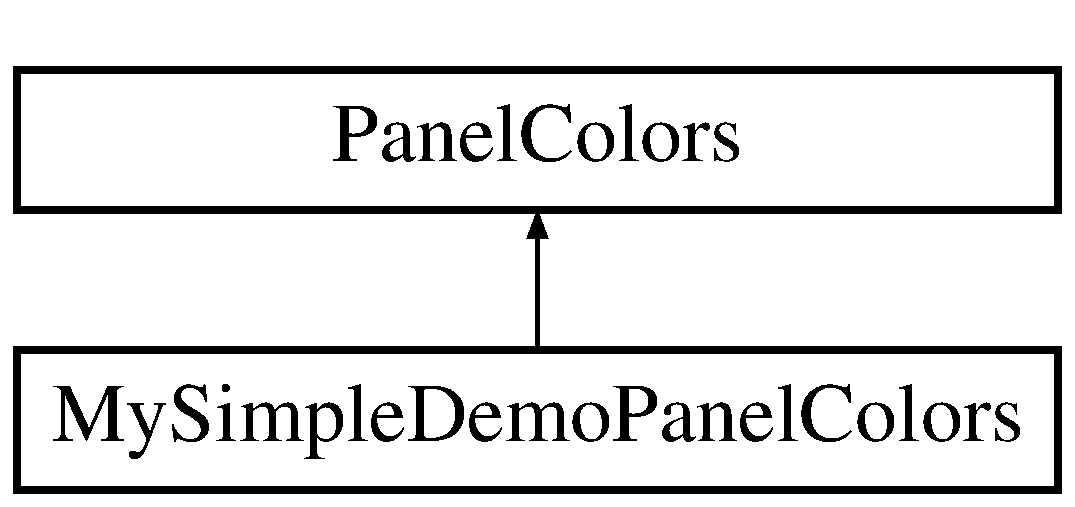
\includegraphics[height=2.000000cm]{struct_my_simple_demo_panel_colors}
\end{center}
\end{figure}
\subsection*{Public Member Functions}
\begin{DoxyCompactItemize}
\item 
\hyperlink{struct_my_simple_demo_panel_colors_ad2b47e83124a07e5ede8418915bd25a4}{My\-Simple\-Demo\-Panel\-Colors} ()
\end{DoxyCompactItemize}


\subsection{Detailed Description}
struct. \hyperlink{struct_my_simple_demo_panel_colors}{My\-Simple\-Demo\-Panel\-Colors} desc. Example of customisation of Gui3\-D colors 

\subsection{Constructor \& Destructor Documentation}
\hypertarget{struct_my_simple_demo_panel_colors_ad2b47e83124a07e5ede8418915bd25a4}{\index{My\-Simple\-Demo\-Panel\-Colors@{My\-Simple\-Demo\-Panel\-Colors}!My\-Simple\-Demo\-Panel\-Colors@{My\-Simple\-Demo\-Panel\-Colors}}
\index{My\-Simple\-Demo\-Panel\-Colors@{My\-Simple\-Demo\-Panel\-Colors}!MySimpleDemoPanelColors@{My\-Simple\-Demo\-Panel\-Colors}}
\subsubsection[{My\-Simple\-Demo\-Panel\-Colors}]{\setlength{\rightskip}{0pt plus 5cm}My\-Simple\-Demo\-Panel\-Colors\-::\-My\-Simple\-Demo\-Panel\-Colors (
\begin{DoxyParamCaption}
{}
\end{DoxyParamCaption}
)}}\label{struct_my_simple_demo_panel_colors_ad2b47e83124a07e5ede8418915bd25a4}


The documentation for this struct was generated from the following file\-:\begin{DoxyCompactItemize}
\item 
C\-:/\-Users/\-Aoibhinn/\-Desktop/finished/\-Project\-Colour/\-Project\-One/\-Project\-One/\-Project\-One/include/\hyperlink{_my_simple_demo_panel_colors_8h}{My\-Simple\-Demo\-Panel\-Colors.\-h}\end{DoxyCompactItemize}

\hypertarget{class_project_one}{\section{Project\-One Class Reference}
\label{class_project_one}\index{Project\-One@{Project\-One}}
}


{\ttfamily \#include $<$Project\-One.\-h$>$}

Inheritance diagram for Project\-One\-:\begin{figure}[H]
\begin{center}
\leavevmode
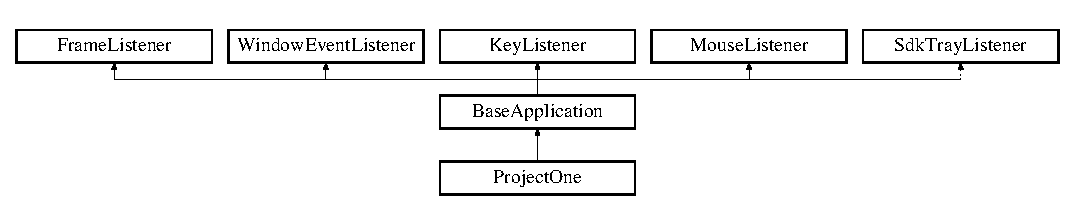
\includegraphics[height=2.382979cm]{class_project_one}
\end{center}
\end{figure}
\subsection*{Public Member Functions}
\begin{DoxyCompactItemize}
\item 
\hyperlink{class_project_one_ac93fc059b5fc7afe41bbaae53b226736}{Project\-One} (void)
\item 
virtual \hyperlink{class_project_one_a337e981319ab327d670bc37d4fa3f7c2}{$\sim$\-Project\-One} (void)
\end{DoxyCompactItemize}
\subsection*{Protected Member Functions}
\begin{DoxyCompactItemize}
\item 
virtual void \hyperlink{class_project_one_a61b71d677e7e4e3ac80071431b65ca5c}{create\-Scene} (void)
\end{DoxyCompactItemize}
\subsection*{Additional Inherited Members}


\subsection{Constructor \& Destructor Documentation}
\hypertarget{class_project_one_ac93fc059b5fc7afe41bbaae53b226736}{\index{Project\-One@{Project\-One}!Project\-One@{Project\-One}}
\index{Project\-One@{Project\-One}!ProjectOne@{Project\-One}}
\subsubsection[{Project\-One}]{\setlength{\rightskip}{0pt plus 5cm}Project\-One\-::\-Project\-One (
\begin{DoxyParamCaption}
\item[{void}]{}
\end{DoxyParamCaption}
)}}\label{class_project_one_ac93fc059b5fc7afe41bbaae53b226736}
\hypertarget{class_project_one_a337e981319ab327d670bc37d4fa3f7c2}{\index{Project\-One@{Project\-One}!$\sim$\-Project\-One@{$\sim$\-Project\-One}}
\index{$\sim$\-Project\-One@{$\sim$\-Project\-One}!ProjectOne@{Project\-One}}
\subsubsection[{$\sim$\-Project\-One}]{\setlength{\rightskip}{0pt plus 5cm}virtual Project\-One\-::$\sim$\-Project\-One (
\begin{DoxyParamCaption}
\item[{void}]{}
\end{DoxyParamCaption}
)\hspace{0.3cm}{\ttfamily [virtual]}}}\label{class_project_one_a337e981319ab327d670bc37d4fa3f7c2}


\subsection{Member Function Documentation}
\hypertarget{class_project_one_a61b71d677e7e4e3ac80071431b65ca5c}{\index{Project\-One@{Project\-One}!create\-Scene@{create\-Scene}}
\index{create\-Scene@{create\-Scene}!ProjectOne@{Project\-One}}
\subsubsection[{create\-Scene}]{\setlength{\rightskip}{0pt plus 5cm}virtual void Project\-One\-::create\-Scene (
\begin{DoxyParamCaption}
\item[{void}]{}
\end{DoxyParamCaption}
)\hspace{0.3cm}{\ttfamily [protected]}, {\ttfamily [virtual]}}}\label{class_project_one_a61b71d677e7e4e3ac80071431b65ca5c}


Implements \hyperlink{class_base_application_aa97beeb4059b17d0ec22eae33286ec2d}{Base\-Application}.



The documentation for this class was generated from the following file\-:\begin{DoxyCompactItemize}
\item 
C\-:/\-Users/\-Aoibhinn/\-Desktop/finished/\-Project\-Colour/\-Project\-One/\-Project\-One/\-Project\-One/include/\hyperlink{_project_one_8h}{Project\-One.\-h}\end{DoxyCompactItemize}

\hypertarget{classt_shape}{\section{t\-Shape Class Reference}
\label{classt_shape}\index{t\-Shape@{t\-Shape}}
}


{\ttfamily \#include $<$t\-Shape.\-h$>$}

\subsection*{Public Types}
\begin{DoxyCompactItemize}
\item 
enum \hyperlink{classt_shape_a193bb18f526dc3f027748fc231b577ae}{Direction\-Facing} \{ \hyperlink{classt_shape_a193bb18f526dc3f027748fc231b577aeae74a49141e9f311876d422f8016b1a29}{x\-Axis}, 
\hyperlink{classt_shape_a193bb18f526dc3f027748fc231b577aea5e1041e853e5ba9f0ec9461cc76f6fa4}{z\-Axis}
 \}
\end{DoxyCompactItemize}
\subsection*{Public Member Functions}
\begin{DoxyCompactItemize}
\item 
\hyperlink{classt_shape_ad6e92496392d351fee71ffa004e53ec6}{t\-Shape} (Ogre\-::\-Scene\-Manager $\ast$, string, string)
\item 
void \hyperlink{classt_shape_a51c0e39d0e8d89872ba1973e9949d2bd}{Update} (double, O\-I\-S\-::\-Keyboard $\ast$, vector$<$ vector$<$ vector$<$ \hyperlink{class_cube}{Cube} $\ast$ $>$$>$$>$ \&array3\-D, int main\-Tick\-Value)
\item 
void \hyperlink{classt_shape_ab4c52b54568e2934ade12889cbad9023}{rotate\-Right} (double, O\-I\-S\-::\-Keyboard $\ast$, vector$<$ vector$<$ vector$<$ \hyperlink{class_cube}{Cube} $\ast$ $>$$>$$>$ \&array3\-D)
\item 
void \hyperlink{classt_shape_a8ac2a90e601d1c95122d00da5da2e035}{rotate\-Y} (double, O\-I\-S\-::\-Keyboard $\ast$, vector$<$ vector$<$ vector$<$ \hyperlink{class_cube}{Cube} $\ast$ $>$$>$$>$ \&array3\-D)
\item 
void \hyperlink{classt_shape_a4abc7fa2f46c54ad12671cba522baef4}{is\-Dropping} (vector$<$ vector$<$ vector$<$ \hyperlink{class_cube}{Cube} $\ast$ $>$$>$$>$ \&array3\-D)
\end{DoxyCompactItemize}
\subsection*{Public Attributes}
\begin{DoxyCompactItemize}
\item 
int \hyperlink{classt_shape_a2df1bbbd7e785bd17cd4d63e8b3a6869}{cube0boundary\-X}
\item 
int \hyperlink{classt_shape_ac4ca3540f5d00586160f68272f60b060}{cube0boundary\-X2}
\item 
int \hyperlink{classt_shape_a5b7cbdbe623f5a877f84b82b70b5dbbb}{cube1boundary\-X}
\item 
int \hyperlink{classt_shape_afc1aab26cc9f3f2469d8080d3f4db30b}{cube1boundary\-X2}
\item 
int \hyperlink{classt_shape_a7cdc58c460ed0ff531971184532e4964}{cube2boundary\-X}
\item 
int \hyperlink{classt_shape_ad3e402834a2d3c1b95d171a0108c8716}{cube2boundary\-X2}
\item 
int \hyperlink{classt_shape_aa1aac01762ff03d22030cb0ed99189f6}{cube3boundary\-X}
\item 
int \hyperlink{classt_shape_a4c6aff9cf7e8fcc0b0fa8d8a0312f83c}{cube3boundary\-X2}
\item 
int \hyperlink{classt_shape_afe93811926d8189ec7a05f3837946d13}{cell\-X}
\item 
int \hyperlink{classt_shape_ac6f6ca34dbe77edc42bf1063f45704f3}{cell\-Y}
\item 
int \hyperlink{classt_shape_a472e4925e0aaa875df22dab7a6ed3551}{cell\-Z}
\item 
int \hyperlink{classt_shape_a6c726e8afc0847cea65901b74bb0f1a4}{cube0boundary\-Z}
\item 
int \hyperlink{classt_shape_ab587a6654689689ee6b94d10f6105082}{cube0boundary\-Z2}
\item 
int \hyperlink{classt_shape_ae1d93af37253f5dd2e59b35366fdd8ef}{cube1boundary\-Z}
\item 
int \hyperlink{classt_shape_af5ef08112c5ac489c6ab89a445563cbd}{cube1boundary\-Z2}
\item 
int \hyperlink{classt_shape_a16bd5d07b91ee4e24e6344c9241d8f95}{cube2boundary\-Z}
\item 
int \hyperlink{classt_shape_a6c6d6c35143aaa266ff75b76f41e38bc}{cube2boundary\-Z2}
\item 
int \hyperlink{classt_shape_a08534f9b32ceebaa5ca648d30a003d6f}{cube3boundary\-Z}
\item 
int \hyperlink{classt_shape_ac0932463ccf31060b93109584e7b142c}{cube3boundary\-Z2}
\item 
int \hyperlink{classt_shape_a39a906a952b50e774dd199829763ce1f}{cube\-Amount}
\item 
int \hyperlink{classt_shape_ab536ba2d1c2fc3e4f367ecf936e49f14}{cube0\-Boundary\-Y}
\item 
bool \hyperlink{classt_shape_a7c8f00d63a58a51843de002a9652cac7}{shadow\-Off}
\item 
bool \hyperlink{classt_shape_a1bb379051554beb845b42fb441e0939c}{alive}
\item 
bool \hyperlink{classt_shape_a2bafbe715483f3f4da44eafae17aac5f}{rotated\-Y}
\item 
bool \hyperlink{classt_shape_a502388884d8386251696471623158a76}{rotated\-X}
\item 
string \hyperlink{classt_shape_ab461221e1ac0abdef5007a6516303d8e}{my\-Name}
\item 
Ogre\-::\-Timer \hyperlink{classt_shape_ae50ef7ba28f10ebe97ab2c431fa27c08}{rotate\-\_\-timer}
\item 
double \hyperlink{classt_shape_ad7f4f8ddfe299bf838030cbc521acb6f}{rotate\-Tick}
\item 
Ogre\-::\-Timer \hyperlink{classt_shape_a8da32e43eeb8ca2a96682ddfd95de45f}{move\-\_\-timer}
\item 
double \hyperlink{classt_shape_a01c34bd393df7caa86a4ff785a1775bd}{move\-Tick}
\item 
Ogre\-::\-Timer \hyperlink{classt_shape_ade6208b0cd2a248227f8ac43e3c3b494}{\-\_\-timer}
\item 
double \hyperlink{classt_shape_a49dc22290f02a6e6ff0f106ffcb16083}{tick}
\item 
double \hyperlink{classt_shape_ad211ab24428076e438d6c9212cd0daa0}{tick\-Value}
\item 
int \hyperlink{classt_shape_a1692503641320662db249899a96465f4}{cell\-Size}
\item 
bool \hyperlink{classt_shape_a373d44cd6129f88aded56fd7a7ea7e43}{cube\-Ready\-To\-Drop} \mbox{[}4\mbox{]}
\item 
int \hyperlink{classt_shape_a959bedb9443f8d99092fe7e249354068}{time}
\item 
int \hyperlink{classt_shape_a5f192d399b118e50bf47c48f3acbd74c}{z\-Direction}
\item 
int \hyperlink{classt_shape_a7d7596d539b46bd0cf0935a1b49c025f}{x\-Direction}
\item 
int \hyperlink{classt_shape_a5049442ea1c882642d58bc384666a9d7}{y\-Direction}
\item 
vector$<$ \hyperlink{class_cube}{Cube} $\ast$ $>$ \hyperlink{classt_shape_a4007a5ffd638a42923b64d09c5d50a87}{cubes}
\item 
enum \hyperlink{classt_shape_a193bb18f526dc3f027748fc231b577ae}{t\-Shape\-::\-Direction\-Facing} \hyperlink{classt_shape_a989a7205be02a011dae710470973a3c4}{direction\-Facing}
\end{DoxyCompactItemize}


\subsection{Member Enumeration Documentation}
\hypertarget{classt_shape_a193bb18f526dc3f027748fc231b577ae}{\index{t\-Shape@{t\-Shape}!Direction\-Facing@{Direction\-Facing}}
\index{Direction\-Facing@{Direction\-Facing}!tShape@{t\-Shape}}
\subsubsection[{Direction\-Facing}]{\setlength{\rightskip}{0pt plus 5cm}enum {\bf t\-Shape\-::\-Direction\-Facing}}}\label{classt_shape_a193bb18f526dc3f027748fc231b577ae}
keepstrack of the shapes orientation \begin{Desc}
\item[Enumerator]\par
\begin{description}
\index{x\-Axis@{x\-Axis}!t\-Shape@{t\-Shape}}\index{t\-Shape@{t\-Shape}!x\-Axis@{x\-Axis}}\item[{\em 
\hypertarget{classt_shape_a193bb18f526dc3f027748fc231b577aeae74a49141e9f311876d422f8016b1a29}{x\-Axis}\label{classt_shape_a193bb18f526dc3f027748fc231b577aeae74a49141e9f311876d422f8016b1a29}
}]\index{z\-Axis@{z\-Axis}!t\-Shape@{t\-Shape}}\index{t\-Shape@{t\-Shape}!z\-Axis@{z\-Axis}}\item[{\em 
\hypertarget{classt_shape_a193bb18f526dc3f027748fc231b577aea5e1041e853e5ba9f0ec9461cc76f6fa4}{z\-Axis}\label{classt_shape_a193bb18f526dc3f027748fc231b577aea5e1041e853e5ba9f0ec9461cc76f6fa4}
}]\end{description}
\end{Desc}


\subsection{Constructor \& Destructor Documentation}
\hypertarget{classt_shape_ad6e92496392d351fee71ffa004e53ec6}{\index{t\-Shape@{t\-Shape}!t\-Shape@{t\-Shape}}
\index{t\-Shape@{t\-Shape}!tShape@{t\-Shape}}
\subsubsection[{t\-Shape}]{\setlength{\rightskip}{0pt plus 5cm}t\-Shape\-::t\-Shape (
\begin{DoxyParamCaption}
\item[{Ogre\-::\-Scene\-Manager $\ast$}]{, }
\item[{string}]{, }
\item[{string}]{}
\end{DoxyParamCaption}
)}}\label{classt_shape_ad6e92496392d351fee71ffa004e53ec6}
constructor 

\subsection{Member Function Documentation}
\hypertarget{classt_shape_a4abc7fa2f46c54ad12671cba522baef4}{\index{t\-Shape@{t\-Shape}!is\-Dropping@{is\-Dropping}}
\index{is\-Dropping@{is\-Dropping}!tShape@{t\-Shape}}
\subsubsection[{is\-Dropping}]{\setlength{\rightskip}{0pt plus 5cm}void t\-Shape\-::is\-Dropping (
\begin{DoxyParamCaption}
\item[{vector$<$ vector$<$ vector$<$ {\bf Cube} $\ast$ $>$$>$$>$ \&}]{array3\-D}
\end{DoxyParamCaption}
)}}\label{classt_shape_a4abc7fa2f46c54ad12671cba522baef4}
makes the cube drop method \hypertarget{classt_shape_ab4c52b54568e2934ade12889cbad9023}{\index{t\-Shape@{t\-Shape}!rotate\-Right@{rotate\-Right}}
\index{rotate\-Right@{rotate\-Right}!tShape@{t\-Shape}}
\subsubsection[{rotate\-Right}]{\setlength{\rightskip}{0pt plus 5cm}void t\-Shape\-::rotate\-Right (
\begin{DoxyParamCaption}
\item[{double}]{, }
\item[{O\-I\-S\-::\-Keyboard $\ast$}]{, }
\item[{vector$<$ vector$<$ vector$<$ {\bf Cube} $\ast$ $>$$>$$>$ \&}]{array3\-D}
\end{DoxyParamCaption}
)}}\label{classt_shape_ab4c52b54568e2934ade12889cbad9023}
rotates the shape method \hypertarget{classt_shape_a8ac2a90e601d1c95122d00da5da2e035}{\index{t\-Shape@{t\-Shape}!rotate\-Y@{rotate\-Y}}
\index{rotate\-Y@{rotate\-Y}!tShape@{t\-Shape}}
\subsubsection[{rotate\-Y}]{\setlength{\rightskip}{0pt plus 5cm}void t\-Shape\-::rotate\-Y (
\begin{DoxyParamCaption}
\item[{double}]{, }
\item[{O\-I\-S\-::\-Keyboard $\ast$}]{, }
\item[{vector$<$ vector$<$ vector$<$ {\bf Cube} $\ast$ $>$$>$$>$ \&}]{array3\-D}
\end{DoxyParamCaption}
)}}\label{classt_shape_a8ac2a90e601d1c95122d00da5da2e035}
rotates the shape method \hypertarget{classt_shape_a51c0e39d0e8d89872ba1973e9949d2bd}{\index{t\-Shape@{t\-Shape}!Update@{Update}}
\index{Update@{Update}!tShape@{t\-Shape}}
\subsubsection[{Update}]{\setlength{\rightskip}{0pt plus 5cm}void t\-Shape\-::\-Update (
\begin{DoxyParamCaption}
\item[{double}]{, }
\item[{O\-I\-S\-::\-Keyboard $\ast$}]{, }
\item[{vector$<$ vector$<$ vector$<$ {\bf Cube} $\ast$ $>$$>$$>$ \&}]{array3\-D, }
\item[{int}]{main\-Tick\-Value}
\end{DoxyParamCaption}
)}}\label{classt_shape_a51c0e39d0e8d89872ba1973e9949d2bd}
update method 

\subsection{Member Data Documentation}
\hypertarget{classt_shape_ade6208b0cd2a248227f8ac43e3c3b494}{\index{t\-Shape@{t\-Shape}!\-\_\-timer@{\-\_\-timer}}
\index{\-\_\-timer@{\-\_\-timer}!tShape@{t\-Shape}}
\subsubsection[{\-\_\-timer}]{\setlength{\rightskip}{0pt plus 5cm}Ogre\-::\-Timer t\-Shape\-::\-\_\-timer}}\label{classt_shape_ade6208b0cd2a248227f8ac43e3c3b494}
oger timer \hypertarget{classt_shape_a1bb379051554beb845b42fb441e0939c}{\index{t\-Shape@{t\-Shape}!alive@{alive}}
\index{alive@{alive}!tShape@{t\-Shape}}
\subsubsection[{alive}]{\setlength{\rightskip}{0pt plus 5cm}bool t\-Shape\-::alive}}\label{classt_shape_a1bb379051554beb845b42fb441e0939c}
tracks if alive or not \hypertarget{classt_shape_a1692503641320662db249899a96465f4}{\index{t\-Shape@{t\-Shape}!cell\-Size@{cell\-Size}}
\index{cell\-Size@{cell\-Size}!tShape@{t\-Shape}}
\subsubsection[{cell\-Size}]{\setlength{\rightskip}{0pt plus 5cm}int t\-Shape\-::cell\-Size}}\label{classt_shape_a1692503641320662db249899a96465f4}
stores the size of a matrix cell \hypertarget{classt_shape_afe93811926d8189ec7a05f3837946d13}{\index{t\-Shape@{t\-Shape}!cell\-X@{cell\-X}}
\index{cell\-X@{cell\-X}!tShape@{t\-Shape}}
\subsubsection[{cell\-X}]{\setlength{\rightskip}{0pt plus 5cm}int t\-Shape\-::cell\-X}}\label{classt_shape_afe93811926d8189ec7a05f3837946d13}
stores m\-\_\-postion.\-X \hypertarget{classt_shape_ac6f6ca34dbe77edc42bf1063f45704f3}{\index{t\-Shape@{t\-Shape}!cell\-Y@{cell\-Y}}
\index{cell\-Y@{cell\-Y}!tShape@{t\-Shape}}
\subsubsection[{cell\-Y}]{\setlength{\rightskip}{0pt plus 5cm}int t\-Shape\-::cell\-Y}}\label{classt_shape_ac6f6ca34dbe77edc42bf1063f45704f3}
stores m\-\_\-postion.\-Y \hypertarget{classt_shape_a472e4925e0aaa875df22dab7a6ed3551}{\index{t\-Shape@{t\-Shape}!cell\-Z@{cell\-Z}}
\index{cell\-Z@{cell\-Z}!tShape@{t\-Shape}}
\subsubsection[{cell\-Z}]{\setlength{\rightskip}{0pt plus 5cm}int t\-Shape\-::cell\-Z}}\label{classt_shape_a472e4925e0aaa875df22dab7a6ed3551}
stores m\-\_\-postion.\-Z \hypertarget{classt_shape_a2df1bbbd7e785bd17cd4d63e8b3a6869}{\index{t\-Shape@{t\-Shape}!cube0boundary\-X@{cube0boundary\-X}}
\index{cube0boundary\-X@{cube0boundary\-X}!tShape@{t\-Shape}}
\subsubsection[{cube0boundary\-X}]{\setlength{\rightskip}{0pt plus 5cm}int t\-Shape\-::cube0boundary\-X}}\label{classt_shape_a2df1bbbd7e785bd17cd4d63e8b3a6869}
keeps the cube at postion 0 inside the matrix \hypertarget{classt_shape_ac4ca3540f5d00586160f68272f60b060}{\index{t\-Shape@{t\-Shape}!cube0boundary\-X2@{cube0boundary\-X2}}
\index{cube0boundary\-X2@{cube0boundary\-X2}!tShape@{t\-Shape}}
\subsubsection[{cube0boundary\-X2}]{\setlength{\rightskip}{0pt plus 5cm}int t\-Shape\-::cube0boundary\-X2}}\label{classt_shape_ac4ca3540f5d00586160f68272f60b060}
\hypertarget{classt_shape_ab536ba2d1c2fc3e4f367ecf936e49f14}{\index{t\-Shape@{t\-Shape}!cube0\-Boundary\-Y@{cube0\-Boundary\-Y}}
\index{cube0\-Boundary\-Y@{cube0\-Boundary\-Y}!tShape@{t\-Shape}}
\subsubsection[{cube0\-Boundary\-Y}]{\setlength{\rightskip}{0pt plus 5cm}int t\-Shape\-::cube0\-Boundary\-Y}}\label{classt_shape_ab536ba2d1c2fc3e4f367ecf936e49f14}
keeps the cube at postion 0 inside the matrix \hypertarget{classt_shape_a6c726e8afc0847cea65901b74bb0f1a4}{\index{t\-Shape@{t\-Shape}!cube0boundary\-Z@{cube0boundary\-Z}}
\index{cube0boundary\-Z@{cube0boundary\-Z}!tShape@{t\-Shape}}
\subsubsection[{cube0boundary\-Z}]{\setlength{\rightskip}{0pt plus 5cm}int t\-Shape\-::cube0boundary\-Z}}\label{classt_shape_a6c726e8afc0847cea65901b74bb0f1a4}
keeps the cube at postion 0 inside the matrix \hypertarget{classt_shape_ab587a6654689689ee6b94d10f6105082}{\index{t\-Shape@{t\-Shape}!cube0boundary\-Z2@{cube0boundary\-Z2}}
\index{cube0boundary\-Z2@{cube0boundary\-Z2}!tShape@{t\-Shape}}
\subsubsection[{cube0boundary\-Z2}]{\setlength{\rightskip}{0pt plus 5cm}int t\-Shape\-::cube0boundary\-Z2}}\label{classt_shape_ab587a6654689689ee6b94d10f6105082}
\hypertarget{classt_shape_a5b7cbdbe623f5a877f84b82b70b5dbbb}{\index{t\-Shape@{t\-Shape}!cube1boundary\-X@{cube1boundary\-X}}
\index{cube1boundary\-X@{cube1boundary\-X}!tShape@{t\-Shape}}
\subsubsection[{cube1boundary\-X}]{\setlength{\rightskip}{0pt plus 5cm}int t\-Shape\-::cube1boundary\-X}}\label{classt_shape_a5b7cbdbe623f5a877f84b82b70b5dbbb}
keeps the cube at postion 1 inside the matrix \hypertarget{classt_shape_afc1aab26cc9f3f2469d8080d3f4db30b}{\index{t\-Shape@{t\-Shape}!cube1boundary\-X2@{cube1boundary\-X2}}
\index{cube1boundary\-X2@{cube1boundary\-X2}!tShape@{t\-Shape}}
\subsubsection[{cube1boundary\-X2}]{\setlength{\rightskip}{0pt plus 5cm}int t\-Shape\-::cube1boundary\-X2}}\label{classt_shape_afc1aab26cc9f3f2469d8080d3f4db30b}
\hypertarget{classt_shape_ae1d93af37253f5dd2e59b35366fdd8ef}{\index{t\-Shape@{t\-Shape}!cube1boundary\-Z@{cube1boundary\-Z}}
\index{cube1boundary\-Z@{cube1boundary\-Z}!tShape@{t\-Shape}}
\subsubsection[{cube1boundary\-Z}]{\setlength{\rightskip}{0pt plus 5cm}int t\-Shape\-::cube1boundary\-Z}}\label{classt_shape_ae1d93af37253f5dd2e59b35366fdd8ef}
keeps the cube at postion 1 inside the matrix \hypertarget{classt_shape_af5ef08112c5ac489c6ab89a445563cbd}{\index{t\-Shape@{t\-Shape}!cube1boundary\-Z2@{cube1boundary\-Z2}}
\index{cube1boundary\-Z2@{cube1boundary\-Z2}!tShape@{t\-Shape}}
\subsubsection[{cube1boundary\-Z2}]{\setlength{\rightskip}{0pt plus 5cm}int t\-Shape\-::cube1boundary\-Z2}}\label{classt_shape_af5ef08112c5ac489c6ab89a445563cbd}
\hypertarget{classt_shape_a7cdc58c460ed0ff531971184532e4964}{\index{t\-Shape@{t\-Shape}!cube2boundary\-X@{cube2boundary\-X}}
\index{cube2boundary\-X@{cube2boundary\-X}!tShape@{t\-Shape}}
\subsubsection[{cube2boundary\-X}]{\setlength{\rightskip}{0pt plus 5cm}int t\-Shape\-::cube2boundary\-X}}\label{classt_shape_a7cdc58c460ed0ff531971184532e4964}
keeps the cube at postion 2 inside the matrix \hypertarget{classt_shape_ad3e402834a2d3c1b95d171a0108c8716}{\index{t\-Shape@{t\-Shape}!cube2boundary\-X2@{cube2boundary\-X2}}
\index{cube2boundary\-X2@{cube2boundary\-X2}!tShape@{t\-Shape}}
\subsubsection[{cube2boundary\-X2}]{\setlength{\rightskip}{0pt plus 5cm}int t\-Shape\-::cube2boundary\-X2}}\label{classt_shape_ad3e402834a2d3c1b95d171a0108c8716}
\hypertarget{classt_shape_a16bd5d07b91ee4e24e6344c9241d8f95}{\index{t\-Shape@{t\-Shape}!cube2boundary\-Z@{cube2boundary\-Z}}
\index{cube2boundary\-Z@{cube2boundary\-Z}!tShape@{t\-Shape}}
\subsubsection[{cube2boundary\-Z}]{\setlength{\rightskip}{0pt plus 5cm}int t\-Shape\-::cube2boundary\-Z}}\label{classt_shape_a16bd5d07b91ee4e24e6344c9241d8f95}
keeps the cube at postion 2 inside the matrix \hypertarget{classt_shape_a6c6d6c35143aaa266ff75b76f41e38bc}{\index{t\-Shape@{t\-Shape}!cube2boundary\-Z2@{cube2boundary\-Z2}}
\index{cube2boundary\-Z2@{cube2boundary\-Z2}!tShape@{t\-Shape}}
\subsubsection[{cube2boundary\-Z2}]{\setlength{\rightskip}{0pt plus 5cm}int t\-Shape\-::cube2boundary\-Z2}}\label{classt_shape_a6c6d6c35143aaa266ff75b76f41e38bc}
\hypertarget{classt_shape_aa1aac01762ff03d22030cb0ed99189f6}{\index{t\-Shape@{t\-Shape}!cube3boundary\-X@{cube3boundary\-X}}
\index{cube3boundary\-X@{cube3boundary\-X}!tShape@{t\-Shape}}
\subsubsection[{cube3boundary\-X}]{\setlength{\rightskip}{0pt plus 5cm}int t\-Shape\-::cube3boundary\-X}}\label{classt_shape_aa1aac01762ff03d22030cb0ed99189f6}
keeps the cube at postion 3 inside the matrix \hypertarget{classt_shape_a4c6aff9cf7e8fcc0b0fa8d8a0312f83c}{\index{t\-Shape@{t\-Shape}!cube3boundary\-X2@{cube3boundary\-X2}}
\index{cube3boundary\-X2@{cube3boundary\-X2}!tShape@{t\-Shape}}
\subsubsection[{cube3boundary\-X2}]{\setlength{\rightskip}{0pt plus 5cm}int t\-Shape\-::cube3boundary\-X2}}\label{classt_shape_a4c6aff9cf7e8fcc0b0fa8d8a0312f83c}
\hypertarget{classt_shape_a08534f9b32ceebaa5ca648d30a003d6f}{\index{t\-Shape@{t\-Shape}!cube3boundary\-Z@{cube3boundary\-Z}}
\index{cube3boundary\-Z@{cube3boundary\-Z}!tShape@{t\-Shape}}
\subsubsection[{cube3boundary\-Z}]{\setlength{\rightskip}{0pt plus 5cm}int t\-Shape\-::cube3boundary\-Z}}\label{classt_shape_a08534f9b32ceebaa5ca648d30a003d6f}
keeps the cube at postion 3 inside the matrix \hypertarget{classt_shape_ac0932463ccf31060b93109584e7b142c}{\index{t\-Shape@{t\-Shape}!cube3boundary\-Z2@{cube3boundary\-Z2}}
\index{cube3boundary\-Z2@{cube3boundary\-Z2}!tShape@{t\-Shape}}
\subsubsection[{cube3boundary\-Z2}]{\setlength{\rightskip}{0pt plus 5cm}int t\-Shape\-::cube3boundary\-Z2}}\label{classt_shape_ac0932463ccf31060b93109584e7b142c}
\hypertarget{classt_shape_a39a906a952b50e774dd199829763ce1f}{\index{t\-Shape@{t\-Shape}!cube\-Amount@{cube\-Amount}}
\index{cube\-Amount@{cube\-Amount}!tShape@{t\-Shape}}
\subsubsection[{cube\-Amount}]{\setlength{\rightskip}{0pt plus 5cm}int t\-Shape\-::cube\-Amount}}\label{classt_shape_a39a906a952b50e774dd199829763ce1f}
the amouunt of cubes in the array \hypertarget{classt_shape_a373d44cd6129f88aded56fd7a7ea7e43}{\index{t\-Shape@{t\-Shape}!cube\-Ready\-To\-Drop@{cube\-Ready\-To\-Drop}}
\index{cube\-Ready\-To\-Drop@{cube\-Ready\-To\-Drop}!tShape@{t\-Shape}}
\subsubsection[{cube\-Ready\-To\-Drop}]{\setlength{\rightskip}{0pt plus 5cm}bool t\-Shape\-::cube\-Ready\-To\-Drop\mbox{[}4\mbox{]}}}\label{classt_shape_a373d44cd6129f88aded56fd7a7ea7e43}
tracks if cube readyto drop \hypertarget{classt_shape_a4007a5ffd638a42923b64d09c5d50a87}{\index{t\-Shape@{t\-Shape}!cubes@{cubes}}
\index{cubes@{cubes}!tShape@{t\-Shape}}
\subsubsection[{cubes}]{\setlength{\rightskip}{0pt plus 5cm}vector$<${\bf Cube}$\ast$$>$ t\-Shape\-::cubes}}\label{classt_shape_a4007a5ffd638a42923b64d09c5d50a87}
array of cube objects \hypertarget{classt_shape_a989a7205be02a011dae710470973a3c4}{\index{t\-Shape@{t\-Shape}!direction\-Facing@{direction\-Facing}}
\index{direction\-Facing@{direction\-Facing}!tShape@{t\-Shape}}
\subsubsection[{direction\-Facing}]{\setlength{\rightskip}{0pt plus 5cm}enum {\bf t\-Shape\-::\-Direction\-Facing}  t\-Shape\-::direction\-Facing}}\label{classt_shape_a989a7205be02a011dae710470973a3c4}
\hypertarget{classt_shape_a8da32e43eeb8ca2a96682ddfd95de45f}{\index{t\-Shape@{t\-Shape}!move\-\_\-timer@{move\-\_\-timer}}
\index{move\-\_\-timer@{move\-\_\-timer}!tShape@{t\-Shape}}
\subsubsection[{move\-\_\-timer}]{\setlength{\rightskip}{0pt plus 5cm}Ogre\-::\-Timer t\-Shape\-::move\-\_\-timer}}\label{classt_shape_a8da32e43eeb8ca2a96682ddfd95de45f}
oger timer \hypertarget{classt_shape_a01c34bd393df7caa86a4ff785a1775bd}{\index{t\-Shape@{t\-Shape}!move\-Tick@{move\-Tick}}
\index{move\-Tick@{move\-Tick}!tShape@{t\-Shape}}
\subsubsection[{move\-Tick}]{\setlength{\rightskip}{0pt plus 5cm}double t\-Shape\-::move\-Tick}}\label{classt_shape_a01c34bd393df7caa86a4ff785a1775bd}
stores move tick \hypertarget{classt_shape_ab461221e1ac0abdef5007a6516303d8e}{\index{t\-Shape@{t\-Shape}!my\-Name@{my\-Name}}
\index{my\-Name@{my\-Name}!tShape@{t\-Shape}}
\subsubsection[{my\-Name}]{\setlength{\rightskip}{0pt plus 5cm}string t\-Shape\-::my\-Name}}\label{classt_shape_ab461221e1ac0abdef5007a6516303d8e}
shape name \hypertarget{classt_shape_ae50ef7ba28f10ebe97ab2c431fa27c08}{\index{t\-Shape@{t\-Shape}!rotate\-\_\-timer@{rotate\-\_\-timer}}
\index{rotate\-\_\-timer@{rotate\-\_\-timer}!tShape@{t\-Shape}}
\subsubsection[{rotate\-\_\-timer}]{\setlength{\rightskip}{0pt plus 5cm}Ogre\-::\-Timer t\-Shape\-::rotate\-\_\-timer}}\label{classt_shape_ae50ef7ba28f10ebe97ab2c431fa27c08}
oger timer \hypertarget{classt_shape_a502388884d8386251696471623158a76}{\index{t\-Shape@{t\-Shape}!rotated\-X@{rotated\-X}}
\index{rotated\-X@{rotated\-X}!tShape@{t\-Shape}}
\subsubsection[{rotated\-X}]{\setlength{\rightskip}{0pt plus 5cm}bool t\-Shape\-::rotated\-X}}\label{classt_shape_a502388884d8386251696471623158a76}
rotate\-X \hypertarget{classt_shape_a2bafbe715483f3f4da44eafae17aac5f}{\index{t\-Shape@{t\-Shape}!rotated\-Y@{rotated\-Y}}
\index{rotated\-Y@{rotated\-Y}!tShape@{t\-Shape}}
\subsubsection[{rotated\-Y}]{\setlength{\rightskip}{0pt plus 5cm}bool t\-Shape\-::rotated\-Y}}\label{classt_shape_a2bafbe715483f3f4da44eafae17aac5f}
rotate\-Y \hypertarget{classt_shape_ad7f4f8ddfe299bf838030cbc521acb6f}{\index{t\-Shape@{t\-Shape}!rotate\-Tick@{rotate\-Tick}}
\index{rotate\-Tick@{rotate\-Tick}!tShape@{t\-Shape}}
\subsubsection[{rotate\-Tick}]{\setlength{\rightskip}{0pt plus 5cm}double t\-Shape\-::rotate\-Tick}}\label{classt_shape_ad7f4f8ddfe299bf838030cbc521acb6f}
stores rotate tick \hypertarget{classt_shape_a7c8f00d63a58a51843de002a9652cac7}{\index{t\-Shape@{t\-Shape}!shadow\-Off@{shadow\-Off}}
\index{shadow\-Off@{shadow\-Off}!tShape@{t\-Shape}}
\subsubsection[{shadow\-Off}]{\setlength{\rightskip}{0pt plus 5cm}bool t\-Shape\-::shadow\-Off}}\label{classt_shape_a7c8f00d63a58a51843de002a9652cac7}
checks if shadow is on \hypertarget{classt_shape_a49dc22290f02a6e6ff0f106ffcb16083}{\index{t\-Shape@{t\-Shape}!tick@{tick}}
\index{tick@{tick}!tShape@{t\-Shape}}
\subsubsection[{tick}]{\setlength{\rightskip}{0pt plus 5cm}double t\-Shape\-::tick}}\label{classt_shape_a49dc22290f02a6e6ff0f106ffcb16083}
stores the tick \hypertarget{classt_shape_ad211ab24428076e438d6c9212cd0daa0}{\index{t\-Shape@{t\-Shape}!tick\-Value@{tick\-Value}}
\index{tick\-Value@{tick\-Value}!tShape@{t\-Shape}}
\subsubsection[{tick\-Value}]{\setlength{\rightskip}{0pt plus 5cm}double t\-Shape\-::tick\-Value}}\label{classt_shape_ad211ab24428076e438d6c9212cd0daa0}
stores the tick value \hypertarget{classt_shape_a959bedb9443f8d99092fe7e249354068}{\index{t\-Shape@{t\-Shape}!time@{time}}
\index{time@{time}!tShape@{t\-Shape}}
\subsubsection[{time}]{\setlength{\rightskip}{0pt plus 5cm}int t\-Shape\-::time}}\label{classt_shape_a959bedb9443f8d99092fe7e249354068}
stroes the time value \hypertarget{classt_shape_a7d7596d539b46bd0cf0935a1b49c025f}{\index{t\-Shape@{t\-Shape}!x\-Direction@{x\-Direction}}
\index{x\-Direction@{x\-Direction}!tShape@{t\-Shape}}
\subsubsection[{x\-Direction}]{\setlength{\rightskip}{0pt plus 5cm}int t\-Shape\-::x\-Direction}}\label{classt_shape_a7d7596d539b46bd0cf0935a1b49c025f}
stroes the x\-Direction value \hypertarget{classt_shape_a5049442ea1c882642d58bc384666a9d7}{\index{t\-Shape@{t\-Shape}!y\-Direction@{y\-Direction}}
\index{y\-Direction@{y\-Direction}!tShape@{t\-Shape}}
\subsubsection[{y\-Direction}]{\setlength{\rightskip}{0pt plus 5cm}int t\-Shape\-::y\-Direction}}\label{classt_shape_a5049442ea1c882642d58bc384666a9d7}
stroes the y\-Direction value \hypertarget{classt_shape_a5f192d399b118e50bf47c48f3acbd74c}{\index{t\-Shape@{t\-Shape}!z\-Direction@{z\-Direction}}
\index{z\-Direction@{z\-Direction}!tShape@{t\-Shape}}
\subsubsection[{z\-Direction}]{\setlength{\rightskip}{0pt plus 5cm}int t\-Shape\-::z\-Direction}}\label{classt_shape_a5f192d399b118e50bf47c48f3acbd74c}
stroes the z\-Direction value 

The documentation for this class was generated from the following file\-:\begin{DoxyCompactItemize}
\item 
C\-:/\-Users/\-Aoibhinn/\-Desktop/finished/\-Project\-Colour/\-Project\-One/\-Project\-One/\-Project\-One/include/\hyperlink{t_shape_8h}{t\-Shape.\-h}\end{DoxyCompactItemize}

\hypertarget{classt_shape_opp}{\section{t\-Shape\-Opp Class Reference}
\label{classt_shape_opp}\index{t\-Shape\-Opp@{t\-Shape\-Opp}}
}


{\ttfamily \#include $<$t\-Shape\-Opp.\-h$>$}

\subsection*{Public Types}
\begin{DoxyCompactItemize}
\item 
enum \hyperlink{classt_shape_opp_a066c267390282f939cd988fadd2e3516}{Direction\-Facing} \{ \hyperlink{classt_shape_opp_a066c267390282f939cd988fadd2e3516ae8e3655442885a1fe4b2d4951b3c1767}{right}, 
\hyperlink{classt_shape_opp_a066c267390282f939cd988fadd2e3516a8764600d2854435bef463aa469ac1ac9}{left}, 
\hyperlink{classt_shape_opp_a066c267390282f939cd988fadd2e3516a1ce45a471c6ed53c1474ff7894ea0379}{backwards}, 
\hyperlink{classt_shape_opp_a066c267390282f939cd988fadd2e3516a2a7d593d8ee3566010d630176832245c}{forwards}
 \}
\end{DoxyCompactItemize}
\subsection*{Public Member Functions}
\begin{DoxyCompactItemize}
\item 
\hyperlink{classt_shape_opp_a81365e8a9906035bf34f5b5f56b68e48}{t\-Shape\-Opp} (Ogre\-::\-Scene\-Manager $\ast$, string, string)
\item 
void \hyperlink{classt_shape_opp_aa0cf574d15ff12b0c93ba341f56245e4}{Update} (double, O\-I\-S\-::\-Keyboard $\ast$, vector$<$ vector$<$ vector$<$ \hyperlink{class_cube}{Cube} $\ast$ $>$$>$$>$ \&array3\-D, int main\-Tick\-Value)
\item 
void \hyperlink{classt_shape_opp_a4c7791edd5968486a0507f169320056b}{rotate\-Right} (double, O\-I\-S\-::\-Keyboard $\ast$, vector$<$ vector$<$ vector$<$ \hyperlink{class_cube}{Cube} $\ast$ $>$$>$$>$ \&array3\-D)
\item 
void \hyperlink{classt_shape_opp_a91addaaf2c83610b0d0239c9df906282}{rotate\-Left} (double, O\-I\-S\-::\-Keyboard $\ast$, vector$<$ vector$<$ vector$<$ \hyperlink{class_cube}{Cube} $\ast$ $>$$>$$>$ \&array3\-D)
\item 
void \hyperlink{classt_shape_opp_acdfea913b9c1928a1809a03a86ddd3b7}{is\-Dropping} (vector$<$ vector$<$ vector$<$ \hyperlink{class_cube}{Cube} $\ast$ $>$$>$$>$ \&array3\-D)
\item 
void \hyperlink{classt_shape_opp_aeb23e299c01ad10e4d6cabdc753e5b6d}{Check\-Bounds} ()
\end{DoxyCompactItemize}
\subsection*{Public Attributes}
\begin{DoxyCompactItemize}
\item 
int \hyperlink{classt_shape_opp_a2862f3eed71b35986b016c90c4b05789}{cube0boundary\-X}
\item 
int \hyperlink{classt_shape_opp_aa32382ad78df3bb4bc348615d0ddf861}{cube0boundary\-X2}
\item 
int \hyperlink{classt_shape_opp_afa127f50226a5f01e41b18c91c40cce8}{cube1boundary\-X}
\item 
int \hyperlink{classt_shape_opp_ab2f433b6dc6d22189a2a2f1c9e21bb20}{cube1boundary\-X2}
\item 
int \hyperlink{classt_shape_opp_aab0828a599cc0413a094f9a24c7fa1c6}{cube2boundary\-X}
\item 
int \hyperlink{classt_shape_opp_a0db9ec91d9aa41c32da9489b3a8b01e0}{cube2boundary\-X2}
\item 
int \hyperlink{classt_shape_opp_a3113171f6066946e0817dbb4a0778cab}{cube3boundary\-X}
\item 
int \hyperlink{classt_shape_opp_a26f9cbcb3f5690e3a7d93d3ac94fbadc}{cube3boundary\-X2}
\item 
int \hyperlink{classt_shape_opp_a756674e874a132a61a6fe042f0306cc6}{cell\-X}
\item 
int \hyperlink{classt_shape_opp_a7b383ccd61c7e9f6476dd74e34b747b3}{cell\-Y}
\item 
int \hyperlink{classt_shape_opp_a2e5cae84204ba6ffa6ac65adefd53655}{cell\-Z}
\item 
int \hyperlink{classt_shape_opp_ab87445197fb1652f5af61c8427bdfdf1}{cube0boundary\-Z}
\item 
int \hyperlink{classt_shape_opp_a73e00f928ce84f42cbb9732df4d0b434}{cube0boundary\-Z2}
\item 
int \hyperlink{classt_shape_opp_ad84f70c328391c2775a208953704cefb}{cube1boundary\-Z}
\item 
int \hyperlink{classt_shape_opp_a98286d5bc88ae6f7e44dd3b4a396bb2c}{cube1boundary\-Z2}
\item 
int \hyperlink{classt_shape_opp_a34e02802f83b7d5d08b6a3e76147fbd2}{cube2boundary\-Z}
\item 
int \hyperlink{classt_shape_opp_a95aaa0195ab9dbba7ffda5e90c313b21}{cube2boundary\-Z2}
\item 
int \hyperlink{classt_shape_opp_a899b1d8e9282327163c84c8bae66c1c0}{cube3boundary\-Z}
\item 
int \hyperlink{classt_shape_opp_ab8ac52836e7f0798ed681b2ad862fbde}{cube3boundary\-Z2}
\item 
int \hyperlink{classt_shape_opp_abbdce7342b078dbd08d4fb8f3ce3b8ba}{cube\-Amount}
\item 
int \hyperlink{classt_shape_opp_aa09d7e2bf091902223eca13949282a3b}{cube0\-Boundary\-Y}
\item 
bool \hyperlink{classt_shape_opp_a90ab18a9bba27843937b91a8b03373bf}{shadow\-Off}
\item 
bool \hyperlink{classt_shape_opp_a24e206508358cfc34eef58a0fbb06435}{alive}
\item 
bool \hyperlink{classt_shape_opp_a92e70064fa7e0acbeb04e0821a1b1632}{rotated\-Y}
\item 
bool \hyperlink{classt_shape_opp_a01a922dad69591ec971aaf498d96e007}{rotated\-X}
\item 
string \hyperlink{classt_shape_opp_a0de718635fd734d2fa20597af3204527}{my\-Name}
\item 
Ogre\-::\-Timer \hyperlink{classt_shape_opp_a5696ae6155156237e595f099b4af69c2}{rotate\-\_\-timer}
\item 
double \hyperlink{classt_shape_opp_ae0510d4df7a5235e7bddde0f0ca04ce4}{rotate\-Tick}
\item 
Ogre\-::\-Timer \hyperlink{classt_shape_opp_a8df8a55d84408bce712043537c4b365e}{move\-\_\-timer}
\item 
double \hyperlink{classt_shape_opp_aea755ab737fed04de589062464599fd9}{move\-Tick}
\item 
Ogre\-::\-Timer \hyperlink{classt_shape_opp_a2f21d5931a40c7e5f349c62721183235}{\-\_\-timer}
\item 
double \hyperlink{classt_shape_opp_a68eacd52962b267f55bd0c63178615ee}{tick}
\item 
double \hyperlink{classt_shape_opp_a0716861dd8ce6a12339d038645343017}{tick\-Value}
\item 
int \hyperlink{classt_shape_opp_a2ce0ad0fad70827c369fa8ffae698bf3}{cell\-Size}
\item 
int \hyperlink{classt_shape_opp_aaa9b6325b31d0ce4af2e683f08fdc8de}{time}
\item 
int \hyperlink{classt_shape_opp_addec42a18fe788cd51dcc3045ec9a455}{z\-Direction}
\item 
int \hyperlink{classt_shape_opp_ac2eb74adf1ac7743b5c7e9162c398c26}{x\-Direction}
\item 
int \hyperlink{classt_shape_opp_a87294ad6c4634f1ac2ba4492a0951cf3}{y\-Direction}
\item 
vector$<$ \hyperlink{class_cube}{Cube} $\ast$ $>$ \hyperlink{classt_shape_opp_a6e70d444fb805aa6c1f27a3c3bc37e36}{cubes}
\item 
enum \hyperlink{classt_shape_opp_a066c267390282f939cd988fadd2e3516}{t\-Shape\-Opp\-::\-Direction\-Facing} \hyperlink{classt_shape_opp_a65e2aea9c7466331fc8adc48d7eb147c}{direction\-Facing}
\end{DoxyCompactItemize}


\subsection{Member Enumeration Documentation}
\hypertarget{classt_shape_opp_a066c267390282f939cd988fadd2e3516}{\index{t\-Shape\-Opp@{t\-Shape\-Opp}!Direction\-Facing@{Direction\-Facing}}
\index{Direction\-Facing@{Direction\-Facing}!tShapeOpp@{t\-Shape\-Opp}}
\subsubsection[{Direction\-Facing}]{\setlength{\rightskip}{0pt plus 5cm}enum {\bf t\-Shape\-Opp\-::\-Direction\-Facing}}}\label{classt_shape_opp_a066c267390282f939cd988fadd2e3516}
\begin{Desc}
\item[Enumerator]\par
\begin{description}
\index{right@{right}!t\-Shape\-Opp@{t\-Shape\-Opp}}\index{t\-Shape\-Opp@{t\-Shape\-Opp}!right@{right}}\item[{\em 
\hypertarget{classt_shape_opp_a066c267390282f939cd988fadd2e3516ae8e3655442885a1fe4b2d4951b3c1767}{right}\label{classt_shape_opp_a066c267390282f939cd988fadd2e3516ae8e3655442885a1fe4b2d4951b3c1767}
}]\index{left@{left}!t\-Shape\-Opp@{t\-Shape\-Opp}}\index{t\-Shape\-Opp@{t\-Shape\-Opp}!left@{left}}\item[{\em 
\hypertarget{classt_shape_opp_a066c267390282f939cd988fadd2e3516a8764600d2854435bef463aa469ac1ac9}{left}\label{classt_shape_opp_a066c267390282f939cd988fadd2e3516a8764600d2854435bef463aa469ac1ac9}
}]\index{backwards@{backwards}!t\-Shape\-Opp@{t\-Shape\-Opp}}\index{t\-Shape\-Opp@{t\-Shape\-Opp}!backwards@{backwards}}\item[{\em 
\hypertarget{classt_shape_opp_a066c267390282f939cd988fadd2e3516a1ce45a471c6ed53c1474ff7894ea0379}{backwards}\label{classt_shape_opp_a066c267390282f939cd988fadd2e3516a1ce45a471c6ed53c1474ff7894ea0379}
}]\index{forwards@{forwards}!t\-Shape\-Opp@{t\-Shape\-Opp}}\index{t\-Shape\-Opp@{t\-Shape\-Opp}!forwards@{forwards}}\item[{\em 
\hypertarget{classt_shape_opp_a066c267390282f939cd988fadd2e3516a2a7d593d8ee3566010d630176832245c}{forwards}\label{classt_shape_opp_a066c267390282f939cd988fadd2e3516a2a7d593d8ee3566010d630176832245c}
}]\end{description}
\end{Desc}


\subsection{Constructor \& Destructor Documentation}
\hypertarget{classt_shape_opp_a81365e8a9906035bf34f5b5f56b68e48}{\index{t\-Shape\-Opp@{t\-Shape\-Opp}!t\-Shape\-Opp@{t\-Shape\-Opp}}
\index{t\-Shape\-Opp@{t\-Shape\-Opp}!tShapeOpp@{t\-Shape\-Opp}}
\subsubsection[{t\-Shape\-Opp}]{\setlength{\rightskip}{0pt plus 5cm}t\-Shape\-Opp\-::t\-Shape\-Opp (
\begin{DoxyParamCaption}
\item[{Ogre\-::\-Scene\-Manager $\ast$}]{, }
\item[{string}]{, }
\item[{string}]{}
\end{DoxyParamCaption}
)}}\label{classt_shape_opp_a81365e8a9906035bf34f5b5f56b68e48}


\subsection{Member Function Documentation}
\hypertarget{classt_shape_opp_aeb23e299c01ad10e4d6cabdc753e5b6d}{\index{t\-Shape\-Opp@{t\-Shape\-Opp}!Check\-Bounds@{Check\-Bounds}}
\index{Check\-Bounds@{Check\-Bounds}!tShapeOpp@{t\-Shape\-Opp}}
\subsubsection[{Check\-Bounds}]{\setlength{\rightskip}{0pt plus 5cm}void t\-Shape\-Opp\-::\-Check\-Bounds (
\begin{DoxyParamCaption}
{}
\end{DoxyParamCaption}
)}}\label{classt_shape_opp_aeb23e299c01ad10e4d6cabdc753e5b6d}
\hypertarget{classt_shape_opp_acdfea913b9c1928a1809a03a86ddd3b7}{\index{t\-Shape\-Opp@{t\-Shape\-Opp}!is\-Dropping@{is\-Dropping}}
\index{is\-Dropping@{is\-Dropping}!tShapeOpp@{t\-Shape\-Opp}}
\subsubsection[{is\-Dropping}]{\setlength{\rightskip}{0pt plus 5cm}void t\-Shape\-Opp\-::is\-Dropping (
\begin{DoxyParamCaption}
\item[{vector$<$ vector$<$ vector$<$ {\bf Cube} $\ast$ $>$$>$$>$ \&}]{array3\-D}
\end{DoxyParamCaption}
)}}\label{classt_shape_opp_acdfea913b9c1928a1809a03a86ddd3b7}
\hypertarget{classt_shape_opp_a91addaaf2c83610b0d0239c9df906282}{\index{t\-Shape\-Opp@{t\-Shape\-Opp}!rotate\-Left@{rotate\-Left}}
\index{rotate\-Left@{rotate\-Left}!tShapeOpp@{t\-Shape\-Opp}}
\subsubsection[{rotate\-Left}]{\setlength{\rightskip}{0pt plus 5cm}void t\-Shape\-Opp\-::rotate\-Left (
\begin{DoxyParamCaption}
\item[{double}]{, }
\item[{O\-I\-S\-::\-Keyboard $\ast$}]{, }
\item[{vector$<$ vector$<$ vector$<$ {\bf Cube} $\ast$ $>$$>$$>$ \&}]{array3\-D}
\end{DoxyParamCaption}
)}}\label{classt_shape_opp_a91addaaf2c83610b0d0239c9df906282}
\hypertarget{classt_shape_opp_a4c7791edd5968486a0507f169320056b}{\index{t\-Shape\-Opp@{t\-Shape\-Opp}!rotate\-Right@{rotate\-Right}}
\index{rotate\-Right@{rotate\-Right}!tShapeOpp@{t\-Shape\-Opp}}
\subsubsection[{rotate\-Right}]{\setlength{\rightskip}{0pt plus 5cm}void t\-Shape\-Opp\-::rotate\-Right (
\begin{DoxyParamCaption}
\item[{double}]{, }
\item[{O\-I\-S\-::\-Keyboard $\ast$}]{, }
\item[{vector$<$ vector$<$ vector$<$ {\bf Cube} $\ast$ $>$$>$$>$ \&}]{array3\-D}
\end{DoxyParamCaption}
)}}\label{classt_shape_opp_a4c7791edd5968486a0507f169320056b}
\hypertarget{classt_shape_opp_aa0cf574d15ff12b0c93ba341f56245e4}{\index{t\-Shape\-Opp@{t\-Shape\-Opp}!Update@{Update}}
\index{Update@{Update}!tShapeOpp@{t\-Shape\-Opp}}
\subsubsection[{Update}]{\setlength{\rightskip}{0pt plus 5cm}void t\-Shape\-Opp\-::\-Update (
\begin{DoxyParamCaption}
\item[{double}]{, }
\item[{O\-I\-S\-::\-Keyboard $\ast$}]{, }
\item[{vector$<$ vector$<$ vector$<$ {\bf Cube} $\ast$ $>$$>$$>$ \&}]{array3\-D, }
\item[{int}]{main\-Tick\-Value}
\end{DoxyParamCaption}
)}}\label{classt_shape_opp_aa0cf574d15ff12b0c93ba341f56245e4}


\subsection{Member Data Documentation}
\hypertarget{classt_shape_opp_a2f21d5931a40c7e5f349c62721183235}{\index{t\-Shape\-Opp@{t\-Shape\-Opp}!\-\_\-timer@{\-\_\-timer}}
\index{\-\_\-timer@{\-\_\-timer}!tShapeOpp@{t\-Shape\-Opp}}
\subsubsection[{\-\_\-timer}]{\setlength{\rightskip}{0pt plus 5cm}Ogre\-::\-Timer t\-Shape\-Opp\-::\-\_\-timer}}\label{classt_shape_opp_a2f21d5931a40c7e5f349c62721183235}
\hypertarget{classt_shape_opp_a24e206508358cfc34eef58a0fbb06435}{\index{t\-Shape\-Opp@{t\-Shape\-Opp}!alive@{alive}}
\index{alive@{alive}!tShapeOpp@{t\-Shape\-Opp}}
\subsubsection[{alive}]{\setlength{\rightskip}{0pt plus 5cm}bool t\-Shape\-Opp\-::alive}}\label{classt_shape_opp_a24e206508358cfc34eef58a0fbb06435}
\hypertarget{classt_shape_opp_a2ce0ad0fad70827c369fa8ffae698bf3}{\index{t\-Shape\-Opp@{t\-Shape\-Opp}!cell\-Size@{cell\-Size}}
\index{cell\-Size@{cell\-Size}!tShapeOpp@{t\-Shape\-Opp}}
\subsubsection[{cell\-Size}]{\setlength{\rightskip}{0pt plus 5cm}int t\-Shape\-Opp\-::cell\-Size}}\label{classt_shape_opp_a2ce0ad0fad70827c369fa8ffae698bf3}
\hypertarget{classt_shape_opp_a756674e874a132a61a6fe042f0306cc6}{\index{t\-Shape\-Opp@{t\-Shape\-Opp}!cell\-X@{cell\-X}}
\index{cell\-X@{cell\-X}!tShapeOpp@{t\-Shape\-Opp}}
\subsubsection[{cell\-X}]{\setlength{\rightskip}{0pt plus 5cm}int t\-Shape\-Opp\-::cell\-X}}\label{classt_shape_opp_a756674e874a132a61a6fe042f0306cc6}
\hypertarget{classt_shape_opp_a7b383ccd61c7e9f6476dd74e34b747b3}{\index{t\-Shape\-Opp@{t\-Shape\-Opp}!cell\-Y@{cell\-Y}}
\index{cell\-Y@{cell\-Y}!tShapeOpp@{t\-Shape\-Opp}}
\subsubsection[{cell\-Y}]{\setlength{\rightskip}{0pt plus 5cm}int t\-Shape\-Opp\-::cell\-Y}}\label{classt_shape_opp_a7b383ccd61c7e9f6476dd74e34b747b3}
\hypertarget{classt_shape_opp_a2e5cae84204ba6ffa6ac65adefd53655}{\index{t\-Shape\-Opp@{t\-Shape\-Opp}!cell\-Z@{cell\-Z}}
\index{cell\-Z@{cell\-Z}!tShapeOpp@{t\-Shape\-Opp}}
\subsubsection[{cell\-Z}]{\setlength{\rightskip}{0pt plus 5cm}int t\-Shape\-Opp\-::cell\-Z}}\label{classt_shape_opp_a2e5cae84204ba6ffa6ac65adefd53655}
\hypertarget{classt_shape_opp_a2862f3eed71b35986b016c90c4b05789}{\index{t\-Shape\-Opp@{t\-Shape\-Opp}!cube0boundary\-X@{cube0boundary\-X}}
\index{cube0boundary\-X@{cube0boundary\-X}!tShapeOpp@{t\-Shape\-Opp}}
\subsubsection[{cube0boundary\-X}]{\setlength{\rightskip}{0pt plus 5cm}int t\-Shape\-Opp\-::cube0boundary\-X}}\label{classt_shape_opp_a2862f3eed71b35986b016c90c4b05789}
this is entire class is very similar to \hyperlink{classt_shape}{t\-Shape} although has some different bounds checking a rotation \hypertarget{classt_shape_opp_aa32382ad78df3bb4bc348615d0ddf861}{\index{t\-Shape\-Opp@{t\-Shape\-Opp}!cube0boundary\-X2@{cube0boundary\-X2}}
\index{cube0boundary\-X2@{cube0boundary\-X2}!tShapeOpp@{t\-Shape\-Opp}}
\subsubsection[{cube0boundary\-X2}]{\setlength{\rightskip}{0pt plus 5cm}int t\-Shape\-Opp\-::cube0boundary\-X2}}\label{classt_shape_opp_aa32382ad78df3bb4bc348615d0ddf861}
\hypertarget{classt_shape_opp_aa09d7e2bf091902223eca13949282a3b}{\index{t\-Shape\-Opp@{t\-Shape\-Opp}!cube0\-Boundary\-Y@{cube0\-Boundary\-Y}}
\index{cube0\-Boundary\-Y@{cube0\-Boundary\-Y}!tShapeOpp@{t\-Shape\-Opp}}
\subsubsection[{cube0\-Boundary\-Y}]{\setlength{\rightskip}{0pt plus 5cm}int t\-Shape\-Opp\-::cube0\-Boundary\-Y}}\label{classt_shape_opp_aa09d7e2bf091902223eca13949282a3b}
\hypertarget{classt_shape_opp_ab87445197fb1652f5af61c8427bdfdf1}{\index{t\-Shape\-Opp@{t\-Shape\-Opp}!cube0boundary\-Z@{cube0boundary\-Z}}
\index{cube0boundary\-Z@{cube0boundary\-Z}!tShapeOpp@{t\-Shape\-Opp}}
\subsubsection[{cube0boundary\-Z}]{\setlength{\rightskip}{0pt plus 5cm}int t\-Shape\-Opp\-::cube0boundary\-Z}}\label{classt_shape_opp_ab87445197fb1652f5af61c8427bdfdf1}
\hypertarget{classt_shape_opp_a73e00f928ce84f42cbb9732df4d0b434}{\index{t\-Shape\-Opp@{t\-Shape\-Opp}!cube0boundary\-Z2@{cube0boundary\-Z2}}
\index{cube0boundary\-Z2@{cube0boundary\-Z2}!tShapeOpp@{t\-Shape\-Opp}}
\subsubsection[{cube0boundary\-Z2}]{\setlength{\rightskip}{0pt plus 5cm}int t\-Shape\-Opp\-::cube0boundary\-Z2}}\label{classt_shape_opp_a73e00f928ce84f42cbb9732df4d0b434}
\hypertarget{classt_shape_opp_afa127f50226a5f01e41b18c91c40cce8}{\index{t\-Shape\-Opp@{t\-Shape\-Opp}!cube1boundary\-X@{cube1boundary\-X}}
\index{cube1boundary\-X@{cube1boundary\-X}!tShapeOpp@{t\-Shape\-Opp}}
\subsubsection[{cube1boundary\-X}]{\setlength{\rightskip}{0pt plus 5cm}int t\-Shape\-Opp\-::cube1boundary\-X}}\label{classt_shape_opp_afa127f50226a5f01e41b18c91c40cce8}
\hypertarget{classt_shape_opp_ab2f433b6dc6d22189a2a2f1c9e21bb20}{\index{t\-Shape\-Opp@{t\-Shape\-Opp}!cube1boundary\-X2@{cube1boundary\-X2}}
\index{cube1boundary\-X2@{cube1boundary\-X2}!tShapeOpp@{t\-Shape\-Opp}}
\subsubsection[{cube1boundary\-X2}]{\setlength{\rightskip}{0pt plus 5cm}int t\-Shape\-Opp\-::cube1boundary\-X2}}\label{classt_shape_opp_ab2f433b6dc6d22189a2a2f1c9e21bb20}
\hypertarget{classt_shape_opp_ad84f70c328391c2775a208953704cefb}{\index{t\-Shape\-Opp@{t\-Shape\-Opp}!cube1boundary\-Z@{cube1boundary\-Z}}
\index{cube1boundary\-Z@{cube1boundary\-Z}!tShapeOpp@{t\-Shape\-Opp}}
\subsubsection[{cube1boundary\-Z}]{\setlength{\rightskip}{0pt plus 5cm}int t\-Shape\-Opp\-::cube1boundary\-Z}}\label{classt_shape_opp_ad84f70c328391c2775a208953704cefb}
\hypertarget{classt_shape_opp_a98286d5bc88ae6f7e44dd3b4a396bb2c}{\index{t\-Shape\-Opp@{t\-Shape\-Opp}!cube1boundary\-Z2@{cube1boundary\-Z2}}
\index{cube1boundary\-Z2@{cube1boundary\-Z2}!tShapeOpp@{t\-Shape\-Opp}}
\subsubsection[{cube1boundary\-Z2}]{\setlength{\rightskip}{0pt plus 5cm}int t\-Shape\-Opp\-::cube1boundary\-Z2}}\label{classt_shape_opp_a98286d5bc88ae6f7e44dd3b4a396bb2c}
\hypertarget{classt_shape_opp_aab0828a599cc0413a094f9a24c7fa1c6}{\index{t\-Shape\-Opp@{t\-Shape\-Opp}!cube2boundary\-X@{cube2boundary\-X}}
\index{cube2boundary\-X@{cube2boundary\-X}!tShapeOpp@{t\-Shape\-Opp}}
\subsubsection[{cube2boundary\-X}]{\setlength{\rightskip}{0pt plus 5cm}int t\-Shape\-Opp\-::cube2boundary\-X}}\label{classt_shape_opp_aab0828a599cc0413a094f9a24c7fa1c6}
\hypertarget{classt_shape_opp_a0db9ec91d9aa41c32da9489b3a8b01e0}{\index{t\-Shape\-Opp@{t\-Shape\-Opp}!cube2boundary\-X2@{cube2boundary\-X2}}
\index{cube2boundary\-X2@{cube2boundary\-X2}!tShapeOpp@{t\-Shape\-Opp}}
\subsubsection[{cube2boundary\-X2}]{\setlength{\rightskip}{0pt plus 5cm}int t\-Shape\-Opp\-::cube2boundary\-X2}}\label{classt_shape_opp_a0db9ec91d9aa41c32da9489b3a8b01e0}
\hypertarget{classt_shape_opp_a34e02802f83b7d5d08b6a3e76147fbd2}{\index{t\-Shape\-Opp@{t\-Shape\-Opp}!cube2boundary\-Z@{cube2boundary\-Z}}
\index{cube2boundary\-Z@{cube2boundary\-Z}!tShapeOpp@{t\-Shape\-Opp}}
\subsubsection[{cube2boundary\-Z}]{\setlength{\rightskip}{0pt plus 5cm}int t\-Shape\-Opp\-::cube2boundary\-Z}}\label{classt_shape_opp_a34e02802f83b7d5d08b6a3e76147fbd2}
\hypertarget{classt_shape_opp_a95aaa0195ab9dbba7ffda5e90c313b21}{\index{t\-Shape\-Opp@{t\-Shape\-Opp}!cube2boundary\-Z2@{cube2boundary\-Z2}}
\index{cube2boundary\-Z2@{cube2boundary\-Z2}!tShapeOpp@{t\-Shape\-Opp}}
\subsubsection[{cube2boundary\-Z2}]{\setlength{\rightskip}{0pt plus 5cm}int t\-Shape\-Opp\-::cube2boundary\-Z2}}\label{classt_shape_opp_a95aaa0195ab9dbba7ffda5e90c313b21}
\hypertarget{classt_shape_opp_a3113171f6066946e0817dbb4a0778cab}{\index{t\-Shape\-Opp@{t\-Shape\-Opp}!cube3boundary\-X@{cube3boundary\-X}}
\index{cube3boundary\-X@{cube3boundary\-X}!tShapeOpp@{t\-Shape\-Opp}}
\subsubsection[{cube3boundary\-X}]{\setlength{\rightskip}{0pt plus 5cm}int t\-Shape\-Opp\-::cube3boundary\-X}}\label{classt_shape_opp_a3113171f6066946e0817dbb4a0778cab}
\hypertarget{classt_shape_opp_a26f9cbcb3f5690e3a7d93d3ac94fbadc}{\index{t\-Shape\-Opp@{t\-Shape\-Opp}!cube3boundary\-X2@{cube3boundary\-X2}}
\index{cube3boundary\-X2@{cube3boundary\-X2}!tShapeOpp@{t\-Shape\-Opp}}
\subsubsection[{cube3boundary\-X2}]{\setlength{\rightskip}{0pt plus 5cm}int t\-Shape\-Opp\-::cube3boundary\-X2}}\label{classt_shape_opp_a26f9cbcb3f5690e3a7d93d3ac94fbadc}
\hypertarget{classt_shape_opp_a899b1d8e9282327163c84c8bae66c1c0}{\index{t\-Shape\-Opp@{t\-Shape\-Opp}!cube3boundary\-Z@{cube3boundary\-Z}}
\index{cube3boundary\-Z@{cube3boundary\-Z}!tShapeOpp@{t\-Shape\-Opp}}
\subsubsection[{cube3boundary\-Z}]{\setlength{\rightskip}{0pt plus 5cm}int t\-Shape\-Opp\-::cube3boundary\-Z}}\label{classt_shape_opp_a899b1d8e9282327163c84c8bae66c1c0}
\hypertarget{classt_shape_opp_ab8ac52836e7f0798ed681b2ad862fbde}{\index{t\-Shape\-Opp@{t\-Shape\-Opp}!cube3boundary\-Z2@{cube3boundary\-Z2}}
\index{cube3boundary\-Z2@{cube3boundary\-Z2}!tShapeOpp@{t\-Shape\-Opp}}
\subsubsection[{cube3boundary\-Z2}]{\setlength{\rightskip}{0pt plus 5cm}int t\-Shape\-Opp\-::cube3boundary\-Z2}}\label{classt_shape_opp_ab8ac52836e7f0798ed681b2ad862fbde}
\hypertarget{classt_shape_opp_abbdce7342b078dbd08d4fb8f3ce3b8ba}{\index{t\-Shape\-Opp@{t\-Shape\-Opp}!cube\-Amount@{cube\-Amount}}
\index{cube\-Amount@{cube\-Amount}!tShapeOpp@{t\-Shape\-Opp}}
\subsubsection[{cube\-Amount}]{\setlength{\rightskip}{0pt plus 5cm}int t\-Shape\-Opp\-::cube\-Amount}}\label{classt_shape_opp_abbdce7342b078dbd08d4fb8f3ce3b8ba}
\hypertarget{classt_shape_opp_a6e70d444fb805aa6c1f27a3c3bc37e36}{\index{t\-Shape\-Opp@{t\-Shape\-Opp}!cubes@{cubes}}
\index{cubes@{cubes}!tShapeOpp@{t\-Shape\-Opp}}
\subsubsection[{cubes}]{\setlength{\rightskip}{0pt plus 5cm}vector$<${\bf Cube}$\ast$$>$ t\-Shape\-Opp\-::cubes}}\label{classt_shape_opp_a6e70d444fb805aa6c1f27a3c3bc37e36}
\hypertarget{classt_shape_opp_a65e2aea9c7466331fc8adc48d7eb147c}{\index{t\-Shape\-Opp@{t\-Shape\-Opp}!direction\-Facing@{direction\-Facing}}
\index{direction\-Facing@{direction\-Facing}!tShapeOpp@{t\-Shape\-Opp}}
\subsubsection[{direction\-Facing}]{\setlength{\rightskip}{0pt plus 5cm}enum {\bf t\-Shape\-Opp\-::\-Direction\-Facing}  t\-Shape\-Opp\-::direction\-Facing}}\label{classt_shape_opp_a65e2aea9c7466331fc8adc48d7eb147c}
\hypertarget{classt_shape_opp_a8df8a55d84408bce712043537c4b365e}{\index{t\-Shape\-Opp@{t\-Shape\-Opp}!move\-\_\-timer@{move\-\_\-timer}}
\index{move\-\_\-timer@{move\-\_\-timer}!tShapeOpp@{t\-Shape\-Opp}}
\subsubsection[{move\-\_\-timer}]{\setlength{\rightskip}{0pt plus 5cm}Ogre\-::\-Timer t\-Shape\-Opp\-::move\-\_\-timer}}\label{classt_shape_opp_a8df8a55d84408bce712043537c4b365e}
\hypertarget{classt_shape_opp_aea755ab737fed04de589062464599fd9}{\index{t\-Shape\-Opp@{t\-Shape\-Opp}!move\-Tick@{move\-Tick}}
\index{move\-Tick@{move\-Tick}!tShapeOpp@{t\-Shape\-Opp}}
\subsubsection[{move\-Tick}]{\setlength{\rightskip}{0pt plus 5cm}double t\-Shape\-Opp\-::move\-Tick}}\label{classt_shape_opp_aea755ab737fed04de589062464599fd9}
\hypertarget{classt_shape_opp_a0de718635fd734d2fa20597af3204527}{\index{t\-Shape\-Opp@{t\-Shape\-Opp}!my\-Name@{my\-Name}}
\index{my\-Name@{my\-Name}!tShapeOpp@{t\-Shape\-Opp}}
\subsubsection[{my\-Name}]{\setlength{\rightskip}{0pt plus 5cm}string t\-Shape\-Opp\-::my\-Name}}\label{classt_shape_opp_a0de718635fd734d2fa20597af3204527}
\hypertarget{classt_shape_opp_a5696ae6155156237e595f099b4af69c2}{\index{t\-Shape\-Opp@{t\-Shape\-Opp}!rotate\-\_\-timer@{rotate\-\_\-timer}}
\index{rotate\-\_\-timer@{rotate\-\_\-timer}!tShapeOpp@{t\-Shape\-Opp}}
\subsubsection[{rotate\-\_\-timer}]{\setlength{\rightskip}{0pt plus 5cm}Ogre\-::\-Timer t\-Shape\-Opp\-::rotate\-\_\-timer}}\label{classt_shape_opp_a5696ae6155156237e595f099b4af69c2}
\hypertarget{classt_shape_opp_a01a922dad69591ec971aaf498d96e007}{\index{t\-Shape\-Opp@{t\-Shape\-Opp}!rotated\-X@{rotated\-X}}
\index{rotated\-X@{rotated\-X}!tShapeOpp@{t\-Shape\-Opp}}
\subsubsection[{rotated\-X}]{\setlength{\rightskip}{0pt plus 5cm}bool t\-Shape\-Opp\-::rotated\-X}}\label{classt_shape_opp_a01a922dad69591ec971aaf498d96e007}
\hypertarget{classt_shape_opp_a92e70064fa7e0acbeb04e0821a1b1632}{\index{t\-Shape\-Opp@{t\-Shape\-Opp}!rotated\-Y@{rotated\-Y}}
\index{rotated\-Y@{rotated\-Y}!tShapeOpp@{t\-Shape\-Opp}}
\subsubsection[{rotated\-Y}]{\setlength{\rightskip}{0pt plus 5cm}bool t\-Shape\-Opp\-::rotated\-Y}}\label{classt_shape_opp_a92e70064fa7e0acbeb04e0821a1b1632}
\hypertarget{classt_shape_opp_ae0510d4df7a5235e7bddde0f0ca04ce4}{\index{t\-Shape\-Opp@{t\-Shape\-Opp}!rotate\-Tick@{rotate\-Tick}}
\index{rotate\-Tick@{rotate\-Tick}!tShapeOpp@{t\-Shape\-Opp}}
\subsubsection[{rotate\-Tick}]{\setlength{\rightskip}{0pt plus 5cm}double t\-Shape\-Opp\-::rotate\-Tick}}\label{classt_shape_opp_ae0510d4df7a5235e7bddde0f0ca04ce4}
\hypertarget{classt_shape_opp_a90ab18a9bba27843937b91a8b03373bf}{\index{t\-Shape\-Opp@{t\-Shape\-Opp}!shadow\-Off@{shadow\-Off}}
\index{shadow\-Off@{shadow\-Off}!tShapeOpp@{t\-Shape\-Opp}}
\subsubsection[{shadow\-Off}]{\setlength{\rightskip}{0pt plus 5cm}bool t\-Shape\-Opp\-::shadow\-Off}}\label{classt_shape_opp_a90ab18a9bba27843937b91a8b03373bf}
\hypertarget{classt_shape_opp_a68eacd52962b267f55bd0c63178615ee}{\index{t\-Shape\-Opp@{t\-Shape\-Opp}!tick@{tick}}
\index{tick@{tick}!tShapeOpp@{t\-Shape\-Opp}}
\subsubsection[{tick}]{\setlength{\rightskip}{0pt plus 5cm}double t\-Shape\-Opp\-::tick}}\label{classt_shape_opp_a68eacd52962b267f55bd0c63178615ee}
\hypertarget{classt_shape_opp_a0716861dd8ce6a12339d038645343017}{\index{t\-Shape\-Opp@{t\-Shape\-Opp}!tick\-Value@{tick\-Value}}
\index{tick\-Value@{tick\-Value}!tShapeOpp@{t\-Shape\-Opp}}
\subsubsection[{tick\-Value}]{\setlength{\rightskip}{0pt plus 5cm}double t\-Shape\-Opp\-::tick\-Value}}\label{classt_shape_opp_a0716861dd8ce6a12339d038645343017}
\hypertarget{classt_shape_opp_aaa9b6325b31d0ce4af2e683f08fdc8de}{\index{t\-Shape\-Opp@{t\-Shape\-Opp}!time@{time}}
\index{time@{time}!tShapeOpp@{t\-Shape\-Opp}}
\subsubsection[{time}]{\setlength{\rightskip}{0pt plus 5cm}int t\-Shape\-Opp\-::time}}\label{classt_shape_opp_aaa9b6325b31d0ce4af2e683f08fdc8de}
\hypertarget{classt_shape_opp_ac2eb74adf1ac7743b5c7e9162c398c26}{\index{t\-Shape\-Opp@{t\-Shape\-Opp}!x\-Direction@{x\-Direction}}
\index{x\-Direction@{x\-Direction}!tShapeOpp@{t\-Shape\-Opp}}
\subsubsection[{x\-Direction}]{\setlength{\rightskip}{0pt plus 5cm}int t\-Shape\-Opp\-::x\-Direction}}\label{classt_shape_opp_ac2eb74adf1ac7743b5c7e9162c398c26}
\hypertarget{classt_shape_opp_a87294ad6c4634f1ac2ba4492a0951cf3}{\index{t\-Shape\-Opp@{t\-Shape\-Opp}!y\-Direction@{y\-Direction}}
\index{y\-Direction@{y\-Direction}!tShapeOpp@{t\-Shape\-Opp}}
\subsubsection[{y\-Direction}]{\setlength{\rightskip}{0pt plus 5cm}int t\-Shape\-Opp\-::y\-Direction}}\label{classt_shape_opp_a87294ad6c4634f1ac2ba4492a0951cf3}
\hypertarget{classt_shape_opp_addec42a18fe788cd51dcc3045ec9a455}{\index{t\-Shape\-Opp@{t\-Shape\-Opp}!z\-Direction@{z\-Direction}}
\index{z\-Direction@{z\-Direction}!tShapeOpp@{t\-Shape\-Opp}}
\subsubsection[{z\-Direction}]{\setlength{\rightskip}{0pt plus 5cm}int t\-Shape\-Opp\-::z\-Direction}}\label{classt_shape_opp_addec42a18fe788cd51dcc3045ec9a455}


The documentation for this class was generated from the following file\-:\begin{DoxyCompactItemize}
\item 
C\-:/\-Users/\-Aoibhinn/\-Desktop/finished/\-Project\-Colour/\-Project\-One/\-Project\-One/\-Project\-One/include/\hyperlink{t_shape_opp_8h}{t\-Shape\-Opp.\-h}\end{DoxyCompactItemize}

\hypertarget{classz_shape}{\section{z\-Shape Class Reference}
\label{classz_shape}\index{z\-Shape@{z\-Shape}}
}


{\ttfamily \#include $<$z\-Shape.\-h$>$}

\subsection*{Public Types}
\begin{DoxyCompactItemize}
\item 
enum \hyperlink{classz_shape_ab60d2ccafff31987c3134b99ffdfc168}{Direction\-Facing} \{ \hyperlink{classz_shape_ab60d2ccafff31987c3134b99ffdfc168a98b5b9f6eef05dacfae77a1c2c5f673e}{forward}, 
\hyperlink{classz_shape_ab60d2ccafff31987c3134b99ffdfc168a015e7b2c5830dee71428db58cbe54e91}{backward}, 
\hyperlink{classz_shape_ab60d2ccafff31987c3134b99ffdfc168ac37933597ccfb2403963ab3478b1ba02}{left}, 
\hyperlink{classz_shape_ab60d2ccafff31987c3134b99ffdfc168a577911cbdcc7c610f87e71814cfdad6c}{right}
 \}
\end{DoxyCompactItemize}
\subsection*{Public Member Functions}
\begin{DoxyCompactItemize}
\item 
\hyperlink{classz_shape_a43735d5c74aa0ab56ba2dcdc392d5212}{z\-Shape} (Ogre\-::\-Scene\-Manager $\ast$, string m\-Name, string)
\item 
void \hyperlink{classz_shape_a2d6800f8defaa73954657e103257a520}{Update} (double, O\-I\-S\-::\-Keyboard $\ast$, vector$<$ vector$<$ vector$<$ \hyperlink{class_cube}{Cube} $\ast$ $>$$>$$>$ \&array3\-D, int main\-Tick\-Value)
\item 
void \hyperlink{classz_shape_aebd07968a31f6bf2e3378227d3a4f1a7}{rotate\-Right} (double, vector$<$ vector$<$ vector$<$ \hyperlink{class_cube}{Cube} $\ast$ $>$$>$$>$ \&array3\-D)
\item 
void \hyperlink{classz_shape_a6475eb27003e84467d73dea3603520ed}{rotate\-Left} (double, vector$<$ vector$<$ vector$<$ \hyperlink{class_cube}{Cube} $\ast$ $>$$>$$>$ \&array3\-D)
\item 
void \hyperlink{classz_shape_a95fbe17176889608178c1831ade80c16}{is\-Dropping} (vector$<$ vector$<$ vector$<$ \hyperlink{class_cube}{Cube} $\ast$ $>$$>$$>$ \&array3\-D)
\item 
void \hyperlink{classz_shape_ac599f1a0c6920db0ee7fee7bbe2268e9}{check\-Bounds} ()
\end{DoxyCompactItemize}
\subsection*{Public Attributes}
\begin{DoxyCompactItemize}
\item 
int \hyperlink{classz_shape_ab573e49ed92efb74eea99eeb6015a8f0}{cube0boundary\-X}
\item 
int \hyperlink{classz_shape_a40fae2a3019c20406dc8dbbc9613becf}{cube0boundary\-X2}
\item 
int \hyperlink{classz_shape_a86d5935ac17eb4014518b32a0b7d0b20}{cube1boundary\-X}
\item 
int \hyperlink{classz_shape_a5195d555defef38a13c147cde4610124}{cube1boundary\-X2}
\item 
int \hyperlink{classz_shape_aadc304ad5e51018cd0217bc6f0a39165}{cube2boundary\-X}
\item 
int \hyperlink{classz_shape_a803a7236cf186faa5ea0ee7c86639ba7}{cube2boundary\-X2}
\item 
int \hyperlink{classz_shape_aeb96887365de974440f8494c9da2b097}{cube3boundary\-X}
\item 
int \hyperlink{classz_shape_ab3e6d24301edea1a2d7d35ca34d5b6ad}{cube3boundary\-X2}
\item 
int \hyperlink{classz_shape_a1137620e91f77e816ef97e4e2667499b}{cube0boundary\-Z}
\item 
int \hyperlink{classz_shape_a2d03d0e4d7a150d8d0f5370a4514262f}{cube0boundary\-Z2}
\item 
int \hyperlink{classz_shape_ab1ef86f5f194e4d9cd51488b33ed6642}{cube1boundary\-Z}
\item 
int \hyperlink{classz_shape_aec2d4ff13d10eae9c3b8bca21cbe53a6}{cube1boundary\-Z2}
\item 
int \hyperlink{classz_shape_a6e834a60e1cdeef415deae7f9d1af42d}{cube2boundary\-Z}
\item 
int \hyperlink{classz_shape_a125d6ca0a1894e10414668fd7d24a74b}{cube2boundary\-Z2}
\item 
int \hyperlink{classz_shape_ace4bd139f834c009fc28e38d8712cd65}{cube3boundary\-Z}
\item 
int \hyperlink{classz_shape_afdf3c0ed9499a640373394223bcf5c3e}{cube3boundary\-Z2}
\item 
string \hyperlink{classz_shape_a751cf070b6e1b1ee3936020f01beeab3}{my\-Name}
\item 
Ogre\-::\-Timer \hyperlink{classz_shape_ac8cc62dd7693b1b06d49b837b9a95b6e}{rotate\-\_\-timer}
\item 
double \hyperlink{classz_shape_ababb157263bf9c66de983ac1e5ddec6d}{rotate\-Tick}
\item 
Ogre\-::\-Timer \hyperlink{classz_shape_a56e2cca0a696cf28fa4244ce20267fb4}{move\-\_\-timer}
\item 
double \hyperlink{classz_shape_a06a862d298b4fe36236834a39af1d7b4}{move\-Tick}
\item 
Ogre\-::\-Timer \hyperlink{classz_shape_a2e34a7774c32ab986afcb352bee6de9b}{\-\_\-timer}
\item 
double \hyperlink{classz_shape_add03bb3345a58059a1f76a4cfaaedb54}{tick}
\item 
double \hyperlink{classz_shape_af8baf4bfde98df012d1389768d9571b0}{tick\-Value}
\item 
enum \hyperlink{classz_shape_ab60d2ccafff31987c3134b99ffdfc168}{z\-Shape\-::\-Direction\-Facing} \hyperlink{classz_shape_a22d2f5fca91a1b455a17d5e8fbe4a280}{direction\-Facing}
\item 
int \hyperlink{classz_shape_a0437d50ec76bf6fbe2522ead9b3184e0}{cell\-Size}
\item 
int \hyperlink{classz_shape_a772c76f69f30fefa4b8d08a9d1546dba}{time}
\item 
int \hyperlink{classz_shape_a4ec37982be7b7b02dbb92135629218f2}{z\-Direction}
\item 
int \hyperlink{classz_shape_ab05ebfad3001a2ff2747f7e788efaf06}{x\-Direction}
\item 
bool \hyperlink{classz_shape_a1796431468e8e0b2073e28d94bc4c5bd}{alive}
\item 
bool \hyperlink{classz_shape_a893430248d4812e90d8deca062d39820}{shadow\-Off}
\item 
int \hyperlink{classz_shape_a720c53d979680d3ccd67f453cf45be7e}{cube\-Amount}
\item 
int \hyperlink{classz_shape_a6fb508e0180de23b90db911b1bb97003}{half}
\item 
vector$<$ \hyperlink{class_cube}{Cube} $\ast$ $>$ \hyperlink{classz_shape_aa0d1a3c2b46801c1064c43d33094f29e}{cubes}
\end{DoxyCompactItemize}


\subsection{Member Enumeration Documentation}
\hypertarget{classz_shape_ab60d2ccafff31987c3134b99ffdfc168}{\index{z\-Shape@{z\-Shape}!Direction\-Facing@{Direction\-Facing}}
\index{Direction\-Facing@{Direction\-Facing}!zShape@{z\-Shape}}
\subsubsection[{Direction\-Facing}]{\setlength{\rightskip}{0pt plus 5cm}enum {\bf z\-Shape\-::\-Direction\-Facing}}}\label{classz_shape_ab60d2ccafff31987c3134b99ffdfc168}
tracks the orientation of the shape \begin{Desc}
\item[Enumerator]\par
\begin{description}
\index{forward@{forward}!z\-Shape@{z\-Shape}}\index{z\-Shape@{z\-Shape}!forward@{forward}}\item[{\em 
\hypertarget{classz_shape_ab60d2ccafff31987c3134b99ffdfc168a98b5b9f6eef05dacfae77a1c2c5f673e}{forward}\label{classz_shape_ab60d2ccafff31987c3134b99ffdfc168a98b5b9f6eef05dacfae77a1c2c5f673e}
}]\index{backward@{backward}!z\-Shape@{z\-Shape}}\index{z\-Shape@{z\-Shape}!backward@{backward}}\item[{\em 
\hypertarget{classz_shape_ab60d2ccafff31987c3134b99ffdfc168a015e7b2c5830dee71428db58cbe54e91}{backward}\label{classz_shape_ab60d2ccafff31987c3134b99ffdfc168a015e7b2c5830dee71428db58cbe54e91}
}]\index{left@{left}!z\-Shape@{z\-Shape}}\index{z\-Shape@{z\-Shape}!left@{left}}\item[{\em 
\hypertarget{classz_shape_ab60d2ccafff31987c3134b99ffdfc168ac37933597ccfb2403963ab3478b1ba02}{left}\label{classz_shape_ab60d2ccafff31987c3134b99ffdfc168ac37933597ccfb2403963ab3478b1ba02}
}]\index{right@{right}!z\-Shape@{z\-Shape}}\index{z\-Shape@{z\-Shape}!right@{right}}\item[{\em 
\hypertarget{classz_shape_ab60d2ccafff31987c3134b99ffdfc168a577911cbdcc7c610f87e71814cfdad6c}{right}\label{classz_shape_ab60d2ccafff31987c3134b99ffdfc168a577911cbdcc7c610f87e71814cfdad6c}
}]\end{description}
\end{Desc}


\subsection{Constructor \& Destructor Documentation}
\hypertarget{classz_shape_a43735d5c74aa0ab56ba2dcdc392d5212}{\index{z\-Shape@{z\-Shape}!z\-Shape@{z\-Shape}}
\index{z\-Shape@{z\-Shape}!zShape@{z\-Shape}}
\subsubsection[{z\-Shape}]{\setlength{\rightskip}{0pt plus 5cm}z\-Shape\-::z\-Shape (
\begin{DoxyParamCaption}
\item[{Ogre\-::\-Scene\-Manager $\ast$}]{, }
\item[{string}]{m\-Name, }
\item[{string}]{}
\end{DoxyParamCaption}
)}}\label{classz_shape_a43735d5c74aa0ab56ba2dcdc392d5212}
constructor method 

\subsection{Member Function Documentation}
\hypertarget{classz_shape_ac599f1a0c6920db0ee7fee7bbe2268e9}{\index{z\-Shape@{z\-Shape}!check\-Bounds@{check\-Bounds}}
\index{check\-Bounds@{check\-Bounds}!zShape@{z\-Shape}}
\subsubsection[{check\-Bounds}]{\setlength{\rightskip}{0pt plus 5cm}void z\-Shape\-::check\-Bounds (
\begin{DoxyParamCaption}
{}
\end{DoxyParamCaption}
)}}\label{classz_shape_ac599f1a0c6920db0ee7fee7bbe2268e9}
keeps the cube in side the matrix method \hypertarget{classz_shape_a95fbe17176889608178c1831ade80c16}{\index{z\-Shape@{z\-Shape}!is\-Dropping@{is\-Dropping}}
\index{is\-Dropping@{is\-Dropping}!zShape@{z\-Shape}}
\subsubsection[{is\-Dropping}]{\setlength{\rightskip}{0pt plus 5cm}void z\-Shape\-::is\-Dropping (
\begin{DoxyParamCaption}
\item[{vector$<$ vector$<$ vector$<$ {\bf Cube} $\ast$ $>$$>$$>$ \&}]{array3\-D}
\end{DoxyParamCaption}
)}}\label{classz_shape_a95fbe17176889608178c1831ade80c16}
tracks if the cube is dropping method \hypertarget{classz_shape_a6475eb27003e84467d73dea3603520ed}{\index{z\-Shape@{z\-Shape}!rotate\-Left@{rotate\-Left}}
\index{rotate\-Left@{rotate\-Left}!zShape@{z\-Shape}}
\subsubsection[{rotate\-Left}]{\setlength{\rightskip}{0pt plus 5cm}void z\-Shape\-::rotate\-Left (
\begin{DoxyParamCaption}
\item[{double}]{, }
\item[{vector$<$ vector$<$ vector$<$ {\bf Cube} $\ast$ $>$$>$$>$ \&}]{array3\-D}
\end{DoxyParamCaption}
)}}\label{classz_shape_a6475eb27003e84467d73dea3603520ed}
rotate left method \hypertarget{classz_shape_aebd07968a31f6bf2e3378227d3a4f1a7}{\index{z\-Shape@{z\-Shape}!rotate\-Right@{rotate\-Right}}
\index{rotate\-Right@{rotate\-Right}!zShape@{z\-Shape}}
\subsubsection[{rotate\-Right}]{\setlength{\rightskip}{0pt plus 5cm}void z\-Shape\-::rotate\-Right (
\begin{DoxyParamCaption}
\item[{double}]{, }
\item[{vector$<$ vector$<$ vector$<$ {\bf Cube} $\ast$ $>$$>$$>$ \&}]{array3\-D}
\end{DoxyParamCaption}
)}}\label{classz_shape_aebd07968a31f6bf2e3378227d3a4f1a7}
rotate right method \hypertarget{classz_shape_a2d6800f8defaa73954657e103257a520}{\index{z\-Shape@{z\-Shape}!Update@{Update}}
\index{Update@{Update}!zShape@{z\-Shape}}
\subsubsection[{Update}]{\setlength{\rightskip}{0pt plus 5cm}void z\-Shape\-::\-Update (
\begin{DoxyParamCaption}
\item[{double}]{, }
\item[{O\-I\-S\-::\-Keyboard $\ast$}]{, }
\item[{vector$<$ vector$<$ vector$<$ {\bf Cube} $\ast$ $>$$>$$>$ \&}]{array3\-D, }
\item[{int}]{main\-Tick\-Value}
\end{DoxyParamCaption}
)}}\label{classz_shape_a2d6800f8defaa73954657e103257a520}
update method 

\subsection{Member Data Documentation}
\hypertarget{classz_shape_a2e34a7774c32ab986afcb352bee6de9b}{\index{z\-Shape@{z\-Shape}!\-\_\-timer@{\-\_\-timer}}
\index{\-\_\-timer@{\-\_\-timer}!zShape@{z\-Shape}}
\subsubsection[{\-\_\-timer}]{\setlength{\rightskip}{0pt plus 5cm}Ogre\-::\-Timer z\-Shape\-::\-\_\-timer}}\label{classz_shape_a2e34a7774c32ab986afcb352bee6de9b}
ogre timer \hypertarget{classz_shape_a1796431468e8e0b2073e28d94bc4c5bd}{\index{z\-Shape@{z\-Shape}!alive@{alive}}
\index{alive@{alive}!zShape@{z\-Shape}}
\subsubsection[{alive}]{\setlength{\rightskip}{0pt plus 5cm}bool z\-Shape\-::alive}}\label{classz_shape_a1796431468e8e0b2073e28d94bc4c5bd}
tracks if the cube is alive or not \hypertarget{classz_shape_a0437d50ec76bf6fbe2522ead9b3184e0}{\index{z\-Shape@{z\-Shape}!cell\-Size@{cell\-Size}}
\index{cell\-Size@{cell\-Size}!zShape@{z\-Shape}}
\subsubsection[{cell\-Size}]{\setlength{\rightskip}{0pt plus 5cm}int z\-Shape\-::cell\-Size}}\label{classz_shape_a0437d50ec76bf6fbe2522ead9b3184e0}
size of a cell in the matrix \hypertarget{classz_shape_ab573e49ed92efb74eea99eeb6015a8f0}{\index{z\-Shape@{z\-Shape}!cube0boundary\-X@{cube0boundary\-X}}
\index{cube0boundary\-X@{cube0boundary\-X}!zShape@{z\-Shape}}
\subsubsection[{cube0boundary\-X}]{\setlength{\rightskip}{0pt plus 5cm}int z\-Shape\-::cube0boundary\-X}}\label{classz_shape_ab573e49ed92efb74eea99eeb6015a8f0}
keeps the cube at postion 0 inside the matrix \hypertarget{classz_shape_a40fae2a3019c20406dc8dbbc9613becf}{\index{z\-Shape@{z\-Shape}!cube0boundary\-X2@{cube0boundary\-X2}}
\index{cube0boundary\-X2@{cube0boundary\-X2}!zShape@{z\-Shape}}
\subsubsection[{cube0boundary\-X2}]{\setlength{\rightskip}{0pt plus 5cm}int z\-Shape\-::cube0boundary\-X2}}\label{classz_shape_a40fae2a3019c20406dc8dbbc9613becf}
\hypertarget{classz_shape_a1137620e91f77e816ef97e4e2667499b}{\index{z\-Shape@{z\-Shape}!cube0boundary\-Z@{cube0boundary\-Z}}
\index{cube0boundary\-Z@{cube0boundary\-Z}!zShape@{z\-Shape}}
\subsubsection[{cube0boundary\-Z}]{\setlength{\rightskip}{0pt plus 5cm}int z\-Shape\-::cube0boundary\-Z}}\label{classz_shape_a1137620e91f77e816ef97e4e2667499b}
keeps the cube at postion 0 inside the matrix \hypertarget{classz_shape_a2d03d0e4d7a150d8d0f5370a4514262f}{\index{z\-Shape@{z\-Shape}!cube0boundary\-Z2@{cube0boundary\-Z2}}
\index{cube0boundary\-Z2@{cube0boundary\-Z2}!zShape@{z\-Shape}}
\subsubsection[{cube0boundary\-Z2}]{\setlength{\rightskip}{0pt plus 5cm}int z\-Shape\-::cube0boundary\-Z2}}\label{classz_shape_a2d03d0e4d7a150d8d0f5370a4514262f}
\hypertarget{classz_shape_a86d5935ac17eb4014518b32a0b7d0b20}{\index{z\-Shape@{z\-Shape}!cube1boundary\-X@{cube1boundary\-X}}
\index{cube1boundary\-X@{cube1boundary\-X}!zShape@{z\-Shape}}
\subsubsection[{cube1boundary\-X}]{\setlength{\rightskip}{0pt plus 5cm}int z\-Shape\-::cube1boundary\-X}}\label{classz_shape_a86d5935ac17eb4014518b32a0b7d0b20}
keeps the cube at postion 1 inside the matrix \hypertarget{classz_shape_a5195d555defef38a13c147cde4610124}{\index{z\-Shape@{z\-Shape}!cube1boundary\-X2@{cube1boundary\-X2}}
\index{cube1boundary\-X2@{cube1boundary\-X2}!zShape@{z\-Shape}}
\subsubsection[{cube1boundary\-X2}]{\setlength{\rightskip}{0pt plus 5cm}int z\-Shape\-::cube1boundary\-X2}}\label{classz_shape_a5195d555defef38a13c147cde4610124}
\hypertarget{classz_shape_ab1ef86f5f194e4d9cd51488b33ed6642}{\index{z\-Shape@{z\-Shape}!cube1boundary\-Z@{cube1boundary\-Z}}
\index{cube1boundary\-Z@{cube1boundary\-Z}!zShape@{z\-Shape}}
\subsubsection[{cube1boundary\-Z}]{\setlength{\rightskip}{0pt plus 5cm}int z\-Shape\-::cube1boundary\-Z}}\label{classz_shape_ab1ef86f5f194e4d9cd51488b33ed6642}
keeps the cube at postion 1 inside the matrix \hypertarget{classz_shape_aec2d4ff13d10eae9c3b8bca21cbe53a6}{\index{z\-Shape@{z\-Shape}!cube1boundary\-Z2@{cube1boundary\-Z2}}
\index{cube1boundary\-Z2@{cube1boundary\-Z2}!zShape@{z\-Shape}}
\subsubsection[{cube1boundary\-Z2}]{\setlength{\rightskip}{0pt plus 5cm}int z\-Shape\-::cube1boundary\-Z2}}\label{classz_shape_aec2d4ff13d10eae9c3b8bca21cbe53a6}
\hypertarget{classz_shape_aadc304ad5e51018cd0217bc6f0a39165}{\index{z\-Shape@{z\-Shape}!cube2boundary\-X@{cube2boundary\-X}}
\index{cube2boundary\-X@{cube2boundary\-X}!zShape@{z\-Shape}}
\subsubsection[{cube2boundary\-X}]{\setlength{\rightskip}{0pt plus 5cm}int z\-Shape\-::cube2boundary\-X}}\label{classz_shape_aadc304ad5e51018cd0217bc6f0a39165}
keeps the cube at postion 2 inside the matrix \hypertarget{classz_shape_a803a7236cf186faa5ea0ee7c86639ba7}{\index{z\-Shape@{z\-Shape}!cube2boundary\-X2@{cube2boundary\-X2}}
\index{cube2boundary\-X2@{cube2boundary\-X2}!zShape@{z\-Shape}}
\subsubsection[{cube2boundary\-X2}]{\setlength{\rightskip}{0pt plus 5cm}int z\-Shape\-::cube2boundary\-X2}}\label{classz_shape_a803a7236cf186faa5ea0ee7c86639ba7}
\hypertarget{classz_shape_a6e834a60e1cdeef415deae7f9d1af42d}{\index{z\-Shape@{z\-Shape}!cube2boundary\-Z@{cube2boundary\-Z}}
\index{cube2boundary\-Z@{cube2boundary\-Z}!zShape@{z\-Shape}}
\subsubsection[{cube2boundary\-Z}]{\setlength{\rightskip}{0pt plus 5cm}int z\-Shape\-::cube2boundary\-Z}}\label{classz_shape_a6e834a60e1cdeef415deae7f9d1af42d}
keeps the cube at postion 2 inside the matrix \hypertarget{classz_shape_a125d6ca0a1894e10414668fd7d24a74b}{\index{z\-Shape@{z\-Shape}!cube2boundary\-Z2@{cube2boundary\-Z2}}
\index{cube2boundary\-Z2@{cube2boundary\-Z2}!zShape@{z\-Shape}}
\subsubsection[{cube2boundary\-Z2}]{\setlength{\rightskip}{0pt plus 5cm}int z\-Shape\-::cube2boundary\-Z2}}\label{classz_shape_a125d6ca0a1894e10414668fd7d24a74b}
\hypertarget{classz_shape_aeb96887365de974440f8494c9da2b097}{\index{z\-Shape@{z\-Shape}!cube3boundary\-X@{cube3boundary\-X}}
\index{cube3boundary\-X@{cube3boundary\-X}!zShape@{z\-Shape}}
\subsubsection[{cube3boundary\-X}]{\setlength{\rightskip}{0pt plus 5cm}int z\-Shape\-::cube3boundary\-X}}\label{classz_shape_aeb96887365de974440f8494c9da2b097}
keeps the cube at postion 3 inside the matrix \hypertarget{classz_shape_ab3e6d24301edea1a2d7d35ca34d5b6ad}{\index{z\-Shape@{z\-Shape}!cube3boundary\-X2@{cube3boundary\-X2}}
\index{cube3boundary\-X2@{cube3boundary\-X2}!zShape@{z\-Shape}}
\subsubsection[{cube3boundary\-X2}]{\setlength{\rightskip}{0pt plus 5cm}int z\-Shape\-::cube3boundary\-X2}}\label{classz_shape_ab3e6d24301edea1a2d7d35ca34d5b6ad}
\hypertarget{classz_shape_ace4bd139f834c009fc28e38d8712cd65}{\index{z\-Shape@{z\-Shape}!cube3boundary\-Z@{cube3boundary\-Z}}
\index{cube3boundary\-Z@{cube3boundary\-Z}!zShape@{z\-Shape}}
\subsubsection[{cube3boundary\-Z}]{\setlength{\rightskip}{0pt plus 5cm}int z\-Shape\-::cube3boundary\-Z}}\label{classz_shape_ace4bd139f834c009fc28e38d8712cd65}
keeps the cube at postion 3 inside the matrix \hypertarget{classz_shape_afdf3c0ed9499a640373394223bcf5c3e}{\index{z\-Shape@{z\-Shape}!cube3boundary\-Z2@{cube3boundary\-Z2}}
\index{cube3boundary\-Z2@{cube3boundary\-Z2}!zShape@{z\-Shape}}
\subsubsection[{cube3boundary\-Z2}]{\setlength{\rightskip}{0pt plus 5cm}int z\-Shape\-::cube3boundary\-Z2}}\label{classz_shape_afdf3c0ed9499a640373394223bcf5c3e}
\hypertarget{classz_shape_a720c53d979680d3ccd67f453cf45be7e}{\index{z\-Shape@{z\-Shape}!cube\-Amount@{cube\-Amount}}
\index{cube\-Amount@{cube\-Amount}!zShape@{z\-Shape}}
\subsubsection[{cube\-Amount}]{\setlength{\rightskip}{0pt plus 5cm}int z\-Shape\-::cube\-Amount}}\label{classz_shape_a720c53d979680d3ccd67f453cf45be7e}
amount of cubes in the array \hypertarget{classz_shape_aa0d1a3c2b46801c1064c43d33094f29e}{\index{z\-Shape@{z\-Shape}!cubes@{cubes}}
\index{cubes@{cubes}!zShape@{z\-Shape}}
\subsubsection[{cubes}]{\setlength{\rightskip}{0pt plus 5cm}vector$<${\bf Cube}$\ast$$>$ z\-Shape\-::cubes}}\label{classz_shape_aa0d1a3c2b46801c1064c43d33094f29e}
array of cube objects \hypertarget{classz_shape_a22d2f5fca91a1b455a17d5e8fbe4a280}{\index{z\-Shape@{z\-Shape}!direction\-Facing@{direction\-Facing}}
\index{direction\-Facing@{direction\-Facing}!zShape@{z\-Shape}}
\subsubsection[{direction\-Facing}]{\setlength{\rightskip}{0pt plus 5cm}enum {\bf z\-Shape\-::\-Direction\-Facing}  z\-Shape\-::direction\-Facing}}\label{classz_shape_a22d2f5fca91a1b455a17d5e8fbe4a280}
\hypertarget{classz_shape_a6fb508e0180de23b90db911b1bb97003}{\index{z\-Shape@{z\-Shape}!half@{half}}
\index{half@{half}!zShape@{z\-Shape}}
\subsubsection[{half}]{\setlength{\rightskip}{0pt plus 5cm}int z\-Shape\-::half}}\label{classz_shape_a6fb508e0180de23b90db911b1bb97003}
store half \hypertarget{classz_shape_a56e2cca0a696cf28fa4244ce20267fb4}{\index{z\-Shape@{z\-Shape}!move\-\_\-timer@{move\-\_\-timer}}
\index{move\-\_\-timer@{move\-\_\-timer}!zShape@{z\-Shape}}
\subsubsection[{move\-\_\-timer}]{\setlength{\rightskip}{0pt plus 5cm}Ogre\-::\-Timer z\-Shape\-::move\-\_\-timer}}\label{classz_shape_a56e2cca0a696cf28fa4244ce20267fb4}
ogre timer \hypertarget{classz_shape_a06a862d298b4fe36236834a39af1d7b4}{\index{z\-Shape@{z\-Shape}!move\-Tick@{move\-Tick}}
\index{move\-Tick@{move\-Tick}!zShape@{z\-Shape}}
\subsubsection[{move\-Tick}]{\setlength{\rightskip}{0pt plus 5cm}double z\-Shape\-::move\-Tick}}\label{classz_shape_a06a862d298b4fe36236834a39af1d7b4}
tracks the tick \hypertarget{classz_shape_a751cf070b6e1b1ee3936020f01beeab3}{\index{z\-Shape@{z\-Shape}!my\-Name@{my\-Name}}
\index{my\-Name@{my\-Name}!zShape@{z\-Shape}}
\subsubsection[{my\-Name}]{\setlength{\rightskip}{0pt plus 5cm}string z\-Shape\-::my\-Name}}\label{classz_shape_a751cf070b6e1b1ee3936020f01beeab3}
shapes name \hypertarget{classz_shape_ac8cc62dd7693b1b06d49b837b9a95b6e}{\index{z\-Shape@{z\-Shape}!rotate\-\_\-timer@{rotate\-\_\-timer}}
\index{rotate\-\_\-timer@{rotate\-\_\-timer}!zShape@{z\-Shape}}
\subsubsection[{rotate\-\_\-timer}]{\setlength{\rightskip}{0pt plus 5cm}Ogre\-::\-Timer z\-Shape\-::rotate\-\_\-timer}}\label{classz_shape_ac8cc62dd7693b1b06d49b837b9a95b6e}
ogre timer \hypertarget{classz_shape_ababb157263bf9c66de983ac1e5ddec6d}{\index{z\-Shape@{z\-Shape}!rotate\-Tick@{rotate\-Tick}}
\index{rotate\-Tick@{rotate\-Tick}!zShape@{z\-Shape}}
\subsubsection[{rotate\-Tick}]{\setlength{\rightskip}{0pt plus 5cm}double z\-Shape\-::rotate\-Tick}}\label{classz_shape_ababb157263bf9c66de983ac1e5ddec6d}
tracks the tick \hypertarget{classz_shape_a893430248d4812e90d8deca062d39820}{\index{z\-Shape@{z\-Shape}!shadow\-Off@{shadow\-Off}}
\index{shadow\-Off@{shadow\-Off}!zShape@{z\-Shape}}
\subsubsection[{shadow\-Off}]{\setlength{\rightskip}{0pt plus 5cm}bool z\-Shape\-::shadow\-Off}}\label{classz_shape_a893430248d4812e90d8deca062d39820}
tracks if the shadow is on or off \hypertarget{classz_shape_add03bb3345a58059a1f76a4cfaaedb54}{\index{z\-Shape@{z\-Shape}!tick@{tick}}
\index{tick@{tick}!zShape@{z\-Shape}}
\subsubsection[{tick}]{\setlength{\rightskip}{0pt plus 5cm}double z\-Shape\-::tick}}\label{classz_shape_add03bb3345a58059a1f76a4cfaaedb54}
tracks the tick \hypertarget{classz_shape_af8baf4bfde98df012d1389768d9571b0}{\index{z\-Shape@{z\-Shape}!tick\-Value@{tick\-Value}}
\index{tick\-Value@{tick\-Value}!zShape@{z\-Shape}}
\subsubsection[{tick\-Value}]{\setlength{\rightskip}{0pt plus 5cm}double z\-Shape\-::tick\-Value}}\label{classz_shape_af8baf4bfde98df012d1389768d9571b0}
tracks the tick value \hypertarget{classz_shape_a772c76f69f30fefa4b8d08a9d1546dba}{\index{z\-Shape@{z\-Shape}!time@{time}}
\index{time@{time}!zShape@{z\-Shape}}
\subsubsection[{time}]{\setlength{\rightskip}{0pt plus 5cm}int z\-Shape\-::time}}\label{classz_shape_a772c76f69f30fefa4b8d08a9d1546dba}
tracks trime \hypertarget{classz_shape_ab05ebfad3001a2ff2747f7e788efaf06}{\index{z\-Shape@{z\-Shape}!x\-Direction@{x\-Direction}}
\index{x\-Direction@{x\-Direction}!zShape@{z\-Shape}}
\subsubsection[{x\-Direction}]{\setlength{\rightskip}{0pt plus 5cm}int z\-Shape\-::x\-Direction}}\label{classz_shape_ab05ebfad3001a2ff2747f7e788efaf06}
stores x\-Direction \hypertarget{classz_shape_a4ec37982be7b7b02dbb92135629218f2}{\index{z\-Shape@{z\-Shape}!z\-Direction@{z\-Direction}}
\index{z\-Direction@{z\-Direction}!zShape@{z\-Shape}}
\subsubsection[{z\-Direction}]{\setlength{\rightskip}{0pt plus 5cm}int z\-Shape\-::z\-Direction}}\label{classz_shape_a4ec37982be7b7b02dbb92135629218f2}
stores x\-Direction 

The documentation for this class was generated from the following file\-:\begin{DoxyCompactItemize}
\item 
C\-:/\-Users/\-Aoibhinn/\-Desktop/finished/\-Project\-Colour/\-Project\-One/\-Project\-One/\-Project\-One/include/\hyperlink{z_shape_8h}{z\-Shape.\-h}\end{DoxyCompactItemize}

\chapter{File Documentation}
\hypertarget{_base_application_8h}{\section{C\-:/\-Users/\-Aoibhinn/\-Desktop/finished/\-Project\-Colour/\-Project\-One/\-Project\-One/\-Project\-One/include/\-Base\-Application.h File Reference}
\label{_base_application_8h}\index{C\-:/\-Users/\-Aoibhinn/\-Desktop/finished/\-Project\-Colour/\-Project\-One/\-Project\-One/\-Project\-One/include/\-Base\-Application.\-h@{C\-:/\-Users/\-Aoibhinn/\-Desktop/finished/\-Project\-Colour/\-Project\-One/\-Project\-One/\-Project\-One/include/\-Base\-Application.\-h}}
}
{\ttfamily \#include $<$Ogre\-Camera.\-h$>$}\\*
{\ttfamily \#include $<$Ogre\-Entity.\-h$>$}\\*
{\ttfamily \#include $<$Ogre\-Log\-Manager.\-h$>$}\\*
{\ttfamily \#include $<$Ogre\-Root.\-h$>$}\\*
{\ttfamily \#include $<$Ogre\-Viewport.\-h$>$}\\*
{\ttfamily \#include $<$Ogre\-Scene\-Manager.\-h$>$}\\*
{\ttfamily \#include $<$Ogre\-Render\-Window.\-h$>$}\\*
{\ttfamily \#include $<$Ogre\-Config\-File.\-h$>$}\\*
{\ttfamily \#include $<$O\-I\-S\-Events.\-h$>$}\\*
{\ttfamily \#include $<$O\-I\-S\-Input\-Manager.\-h$>$}\\*
{\ttfamily \#include $<$O\-I\-S\-Keyboard.\-h$>$}\\*
{\ttfamily \#include $<$O\-I\-S\-Mouse.\-h$>$}\\*
{\ttfamily \#include $<$Sdk\-Trays.\-h$>$}\\*
{\ttfamily \#include $<$Sdk\-Camera\-Man.\-h$>$}\\*
{\ttfamily \#include $<$sstream$>$}\\*
{\ttfamily \#include $<$vector$>$}\\*
{\ttfamily \#include $<$list$>$}\\*
{\ttfamily \#include \char`\"{}fmod.\-hpp\char`\"{}}\\*
{\ttfamily \#include \char`\"{}Gui3\-D.\-h\char`\"{}}\\*
{\ttfamily \#include \char`\"{}Gui3\-D\-Panel.\-h\char`\"{}}\\*
{\ttfamily \#include \char`\"{}My\-Simple\-Demo\-Panel\-Colors.\-h\char`\"{}}\\*
{\ttfamily \#include \char`\"{}Cube.\-h\char`\"{}}\\*
{\ttfamily \#include \char`\"{}z\-Shape.\-h\char`\"{}}\\*
{\ttfamily \#include \char`\"{}box.\-h\char`\"{}}\\*
{\ttfamily \#include \char`\"{}t\-Shape.\-h\char`\"{}}\\*
{\ttfamily \#include \char`\"{}t\-Shape\-Opp.\-h\char`\"{}}\\*
{\ttfamily \#include \char`\"{}l\-Shape.\-h\char`\"{}}\\*
{\ttfamily \#include \char`\"{}l\-Shape\-Opp.\-h\char`\"{}}\\*
\subsection*{Classes}
\begin{DoxyCompactItemize}
\item 
class \hyperlink{class_base_application}{Base\-Application}
\end{DoxyCompactItemize}

\hypertarget{box_8h}{\section{C\-:/\-Users/\-Aoibhinn/\-Desktop/finished/\-Project\-Colour/\-Project\-One/\-Project\-One/\-Project\-One/include/box.h File Reference}
\label{box_8h}\index{C\-:/\-Users/\-Aoibhinn/\-Desktop/finished/\-Project\-Colour/\-Project\-One/\-Project\-One/\-Project\-One/include/box.\-h@{C\-:/\-Users/\-Aoibhinn/\-Desktop/finished/\-Project\-Colour/\-Project\-One/\-Project\-One/\-Project\-One/include/box.\-h}}
}
{\ttfamily \#include \char`\"{}Ogre.\-h\char`\"{}}\\*
{\ttfamily \#include $<$cstdio$>$}\\*
{\ttfamily \#include \char`\"{}Base\-Application.\-h\char`\"{}}\\*
{\ttfamily \#include $<$ctime$>$}\\*
{\ttfamily \#include \char`\"{}Cube.\-h\char`\"{}}\\*
\subsection*{Classes}
\begin{DoxyCompactItemize}
\item 
class \hyperlink{classbox}{box}
\end{DoxyCompactItemize}

\hypertarget{_cube_8h}{\section{C\-:/\-Users/\-Aoibhinn/\-Desktop/finished/\-Project\-Colour/\-Project\-One/\-Project\-One/\-Project\-One/include/\-Cube.h File Reference}
\label{_cube_8h}\index{C\-:/\-Users/\-Aoibhinn/\-Desktop/finished/\-Project\-Colour/\-Project\-One/\-Project\-One/\-Project\-One/include/\-Cube.\-h@{C\-:/\-Users/\-Aoibhinn/\-Desktop/finished/\-Project\-Colour/\-Project\-One/\-Project\-One/\-Project\-One/include/\-Cube.\-h}}
}
{\ttfamily \#include \char`\"{}Ogre.\-h\char`\"{}}\\*
{\ttfamily \#include $<$cstdio$>$}\\*
{\ttfamily \#include \char`\"{}Base\-Application.\-h\char`\"{}}\\*
{\ttfamily \#include $<$ctime$>$}\\*
\subsection*{Classes}
\begin{DoxyCompactItemize}
\item 
class \hyperlink{class_cube}{Cube}
\end{DoxyCompactItemize}

\hypertarget{l_shape_8h}{\section{C\-:/\-Users/\-Aoibhinn/\-Desktop/finished/\-Project\-Colour/\-Project\-One/\-Project\-One/\-Project\-One/include/l\-Shape.h File Reference}
\label{l_shape_8h}\index{C\-:/\-Users/\-Aoibhinn/\-Desktop/finished/\-Project\-Colour/\-Project\-One/\-Project\-One/\-Project\-One/include/l\-Shape.\-h@{C\-:/\-Users/\-Aoibhinn/\-Desktop/finished/\-Project\-Colour/\-Project\-One/\-Project\-One/\-Project\-One/include/l\-Shape.\-h}}
}
{\ttfamily \#include \char`\"{}Ogre.\-h\char`\"{}}\\*
{\ttfamily \#include $<$cstdio$>$}\\*
{\ttfamily \#include \char`\"{}Base\-Application.\-h\char`\"{}}\\*
{\ttfamily \#include $<$ctime$>$}\\*
{\ttfamily \#include \char`\"{}Cube.\-h\char`\"{}}\\*
\subsection*{Classes}
\begin{DoxyCompactItemize}
\item 
class \hyperlink{classl_shape}{l\-Shape}
\end{DoxyCompactItemize}

\hypertarget{l_shape_opp_8h}{\section{C\-:/\-Users/\-Aoibhinn/\-Desktop/finished/\-Project\-Colour/\-Project\-One/\-Project\-One/\-Project\-One/include/l\-Shape\-Opp.h File Reference}
\label{l_shape_opp_8h}\index{C\-:/\-Users/\-Aoibhinn/\-Desktop/finished/\-Project\-Colour/\-Project\-One/\-Project\-One/\-Project\-One/include/l\-Shape\-Opp.\-h@{C\-:/\-Users/\-Aoibhinn/\-Desktop/finished/\-Project\-Colour/\-Project\-One/\-Project\-One/\-Project\-One/include/l\-Shape\-Opp.\-h}}
}
{\ttfamily \#include \char`\"{}Ogre.\-h\char`\"{}}\\*
{\ttfamily \#include $<$cstdio$>$}\\*
{\ttfamily \#include \char`\"{}Base\-Application.\-h\char`\"{}}\\*
{\ttfamily \#include $<$ctime$>$}\\*
{\ttfamily \#include \char`\"{}Cube.\-h\char`\"{}}\\*
\subsection*{Classes}
\begin{DoxyCompactItemize}
\item 
class \hyperlink{classl_shape_opp}{l\-Shape\-Opp}
\end{DoxyCompactItemize}

\hypertarget{_my_simple_demo_panel_colors_8h}{\section{C\-:/\-Users/\-Aoibhinn/\-Desktop/finished/\-Project\-Colour/\-Project\-One/\-Project\-One/\-Project\-One/include/\-My\-Simple\-Demo\-Panel\-Colors.h File Reference}
\label{_my_simple_demo_panel_colors_8h}\index{C\-:/\-Users/\-Aoibhinn/\-Desktop/finished/\-Project\-Colour/\-Project\-One/\-Project\-One/\-Project\-One/include/\-My\-Simple\-Demo\-Panel\-Colors.\-h@{C\-:/\-Users/\-Aoibhinn/\-Desktop/finished/\-Project\-Colour/\-Project\-One/\-Project\-One/\-Project\-One/include/\-My\-Simple\-Demo\-Panel\-Colors.\-h}}
}
{\ttfamily \#include \char`\"{}Gui3\-D\-Panel\-Colors.\-h\char`\"{}}\\*
\subsection*{Classes}
\begin{DoxyCompactItemize}
\item 
struct \hyperlink{struct_my_simple_demo_panel_colors}{My\-Simple\-Demo\-Panel\-Colors}
\end{DoxyCompactItemize}

\hypertarget{_project_one_8h}{\section{C\-:/\-Users/\-Aoibhinn/\-Desktop/finished/\-Project\-Colour/\-Project\-One/\-Project\-One/\-Project\-One/include/\-Project\-One.h File Reference}
\label{_project_one_8h}\index{C\-:/\-Users/\-Aoibhinn/\-Desktop/finished/\-Project\-Colour/\-Project\-One/\-Project\-One/\-Project\-One/include/\-Project\-One.\-h@{C\-:/\-Users/\-Aoibhinn/\-Desktop/finished/\-Project\-Colour/\-Project\-One/\-Project\-One/\-Project\-One/include/\-Project\-One.\-h}}
}
{\ttfamily \#include \char`\"{}Base\-Application.\-h\char`\"{}}\\*
{\ttfamily \#include \char`\"{}../res/resource.\-h\char`\"{}}\\*
\subsection*{Classes}
\begin{DoxyCompactItemize}
\item 
class \hyperlink{class_project_one}{Project\-One}
\end{DoxyCompactItemize}

\hypertarget{t_shape_8h}{\section{C\-:/\-Users/\-Aoibhinn/\-Desktop/finished/\-Project\-Colour/\-Project\-One/\-Project\-One/\-Project\-One/include/t\-Shape.h File Reference}
\label{t_shape_8h}\index{C\-:/\-Users/\-Aoibhinn/\-Desktop/finished/\-Project\-Colour/\-Project\-One/\-Project\-One/\-Project\-One/include/t\-Shape.\-h@{C\-:/\-Users/\-Aoibhinn/\-Desktop/finished/\-Project\-Colour/\-Project\-One/\-Project\-One/\-Project\-One/include/t\-Shape.\-h}}
}
{\ttfamily \#include \char`\"{}Ogre.\-h\char`\"{}}\\*
{\ttfamily \#include $<$cstdio$>$}\\*
{\ttfamily \#include \char`\"{}Base\-Application.\-h\char`\"{}}\\*
{\ttfamily \#include $<$ctime$>$}\\*
{\ttfamily \#include \char`\"{}Cube.\-h\char`\"{}}\\*
\subsection*{Classes}
\begin{DoxyCompactItemize}
\item 
class \hyperlink{classt_shape}{t\-Shape}
\end{DoxyCompactItemize}

\hypertarget{t_shape_opp_8h}{\section{C\-:/\-Users/\-Aoibhinn/\-Desktop/finished/\-Project\-Colour/\-Project\-One/\-Project\-One/\-Project\-One/include/t\-Shape\-Opp.h File Reference}
\label{t_shape_opp_8h}\index{C\-:/\-Users/\-Aoibhinn/\-Desktop/finished/\-Project\-Colour/\-Project\-One/\-Project\-One/\-Project\-One/include/t\-Shape\-Opp.\-h@{C\-:/\-Users/\-Aoibhinn/\-Desktop/finished/\-Project\-Colour/\-Project\-One/\-Project\-One/\-Project\-One/include/t\-Shape\-Opp.\-h}}
}
{\ttfamily \#include \char`\"{}Ogre.\-h\char`\"{}}\\*
{\ttfamily \#include $<$cstdio$>$}\\*
{\ttfamily \#include \char`\"{}Base\-Application.\-h\char`\"{}}\\*
{\ttfamily \#include $<$ctime$>$}\\*
{\ttfamily \#include \char`\"{}Cube.\-h\char`\"{}}\\*
\subsection*{Classes}
\begin{DoxyCompactItemize}
\item 
class \hyperlink{classt_shape_opp}{t\-Shape\-Opp}
\end{DoxyCompactItemize}

\hypertarget{z_shape_8h}{\section{C\-:/\-Users/\-Aoibhinn/\-Desktop/finished/\-Project\-Colour/\-Project\-One/\-Project\-One/\-Project\-One/include/z\-Shape.h File Reference}
\label{z_shape_8h}\index{C\-:/\-Users/\-Aoibhinn/\-Desktop/finished/\-Project\-Colour/\-Project\-One/\-Project\-One/\-Project\-One/include/z\-Shape.\-h@{C\-:/\-Users/\-Aoibhinn/\-Desktop/finished/\-Project\-Colour/\-Project\-One/\-Project\-One/\-Project\-One/include/z\-Shape.\-h}}
}
{\ttfamily \#include \char`\"{}Ogre.\-h\char`\"{}}\\*
{\ttfamily \#include $<$cstdio$>$}\\*
{\ttfamily \#include \char`\"{}Base\-Application.\-h\char`\"{}}\\*
{\ttfamily \#include $<$ctime$>$}\\*
{\ttfamily \#include \char`\"{}Cube.\-h\char`\"{}}\\*
\subsection*{Classes}
\begin{DoxyCompactItemize}
\item 
class \hyperlink{classz_shape}{z\-Shape}
\end{DoxyCompactItemize}

%--- End generated contents ---

% Index
\newpage
\phantomsection
\addcontentsline{toc}{chapter}{Index}
\printindex

\end{document}
